\documentclass[11pt]{article}
\usepackage[T1]{fontenc}
\usepackage[utf8]{inputenc}
\usepackage{lmodern}
\usepackage[margin=1in]{geometry}
\usepackage{amsmath,amssymb,amsthm,mathtools}
\usepackage{microtype}
\usepackage{enumitem}
\usepackage{booktabs,longtable,array,graphicx}
\usepackage{xcolor,tikz}
\usetikzlibrary{arrows.meta,positioning,calc,fit}
\usepackage{xurl}
\usepackage[colorlinks=true,linkcolor=blue!50!black,citecolor=blue!50!black,urlcolor=blue!50!black]{hyperref}
\usepackage[capitalize,noabbrev]{cleveref}
\hypersetup{pdftitle={The Kerr--Newman Penrose Inequality for Axisymmetric Electrovacuum Exteriors},pdfauthor={OpenAI},pdfsubject={A sharp inequality and original-data rigidity for connected outer-area-minimizing horizons}}
\setcounter{tocdepth}{2}
\setcounter{secnumdepth}{3}
\setlength{\emergencystretch}{2em}
\setlist{topsep=4pt,itemsep=2pt}
\numberwithin{equation}{section}
\newtheorem{theorem}{Theorem}[section]
\newtheorem{lemma}[theorem]{Lemma}
\newtheorem{proposition}[theorem]{Proposition}
\newtheorem{corollary}[theorem]{Corollary}
\theoremstyle{definition}
\newtheorem{definition}[theorem]{Definition}
\newtheorem{assumption}[theorem]{Assumption}
\theoremstyle{remark}
\newtheorem{remark}[theorem]{Remark}
\newtheorem{example}[theorem]{Example}
\newcommand{\R}{\mathbb R}
\newcommand{\N}{\mathbb N}
\newcommand{\Z}{\mathbb Z}
\newcommand{\dd}{\mathrm d}
\newcommand{\eps}{\varepsilon}
\newcommand{\cD}{\mathcal D}
\newcommand{\cA}{\mathcal A}
\newcommand{\cT}{\mathcal T}
\newcommand{\cP}{\mathcal P}
\newcommand{\cL}{\mathcal L}
\newcommand{\KN}{Kerr--Newman}
\DeclareMathOperator{\tr}{tr}
\DeclareMathOperator{\divg}{div}
\DeclareMathOperator{\Ric}{Ric}
\DeclareMathOperator{\Hess}{Hess}
\DeclareMathOperator{\supp}{supp}
\DeclareMathOperator{\dist}{dist}
\DeclareMathOperator{\Area}{Area}
\DeclareMathOperator{\Vol}{Vol}
\DeclareMathOperator{\id}{id}
\DeclareMathOperator{\sgn}{sgn}
\DeclarePairedDelimiter{\abs}{\lvert}{\rvert}
\DeclarePairedDelimiter{\norm}{\lVert}{\rVert}
\DeclarePairedDelimiter{\ip}{\langle}{\rangle}
\title{The Kerr--Newman Penrose Inequality\\for Axisymmetric Electrovacuum Exteriors}
\author{OpenAI}
\date{October 5, 2026}

\begin{document}
\maketitle
\begin{abstract}
We prove the sharp Kerr--Newman Penrose inequality
\[
m^2\ge \frac{A}{16\pi}+\frac{Q^2}{2}
       +\frac{\pi(Q^4+4J^2)}{A}.
\]
Here \(Q^2=Q_e^2+Q_b^2\), and \(J\) is the conserved total angular
momentum, including its electromagnetic contribution. The result applies
to smooth axisymmetric electrovacuum exteriors in the stated one-ended
topological and decay class, with a connected outermost, outer-area-minimizing
future marginally outer trapped boundary, Coulomb electromagnetic asymptotics,
zero ADM momentum, and the explicitly assumed physical-area condition
\(A\ge4\pi\sqrt{Q^4+4J^2}\). No maximality assumption is made. On the
strict area branch, equality within this class characterizes the original
data as an admissible spacelike exterior slice of a subextremal dyonic
Kerr--Newman spacetime, with the boundary mapped smoothly to a
future-horizon cross-section or the bifurcation sphere.
\end{abstract}

\section{Introduction}
\label{m:introduction}

For a black-hole exterior, the Penrose inequality compares total mass with the
area of the horizon. Electric and magnetic charge and angular momentum sharpen
the expected lower bound to the mass of the \KN\ black hole with the same
horizon area and conserved quantities. The geometric problem is to obtain this
comparison directly from initial data, without assuming that the data are
stationary or that their second fundamental form has zero trace.

Penrose's proposal relates the mass at spatial infinity to the area
required to enclose a black-hole region, as a consequence expected from
gravitational collapse and cosmic censorship~\cite{Penrose1973}.
In the time-symmetric setting, Huisken and Ilmanen proved the Riemannian
inequality for a connected horizon by weak inverse mean curvature
flow~\cite{HuiskenIlmanen2001}; Bray's conformal flow established the
inequality using the total area of an outermost minimal boundary with
several components~\cite{Bray2001}.
For charged Riemannian data, Khuri, Weinstein and Yamada proved the sharp
inequality with multiple horizon components under the appropriate area
branch condition, together with an upper bound for the area radius
without that condition~\cite{KhuriWeinsteinYamada2017}.

Angular momentum introduces additional boundary and gauge information.
Dain, Khuri, Weinstein and Yamada established mass--charge--angular-momentum
and lower-area bounds for simply connected, axisymmetric maximal data
with two ends~\cite{DainKhuriWeinsteinYamada2013}.
Khuri, Sokolowsky and Weinstein obtained a Penrose-type bound for maximal
axisymmetric data with a connected minimal boundary; their comparison
retains an integral of the horizon data and gives the Kerr--Newman
expression under additional horizon matching
conditions~\cite{KhuriSokolowskyWeinstein2019}.
Their harmonic-map method is a useful starting point for the comparison
developed here.

The deformation and first-variation methods draw on the manuscript
\emph{Equality and rigidity in the spacetime Penrose inequality}~\cite{NeutralExterior2026}.
The related charged companion~\cite{ConditionalCharged2026} incorporates
a numerical theorem whose earlier formulation assumed both a neutral
exterior inequality and a separate elliptic existence input; the companion
proves those inputs internally.
We establish the deformation and equality arguments needed here at
their stated scope; no earlier neutral, charged or rotating Penrose
inequality is assumed as an input.


We prove the connected-horizon, outer-area-minimizing, rest-frame formulation
of the axisymmetric \KN\ Penrose conjecture:
\[
 m^2\ge\frac{A}{16\pi}+\frac{Q^2}{2}
                 +\frac{\pi(Q^4+4J^2)}{A}.
\]
Here \(A\) is the horizon area, \(Q^2=Q_e^2+Q_b^2\), and \(J\) is the
conserved total angular momentum, including the electromagnetic contribution.
Theorem~\ref{m:main} states the precise geometric and asymptotic hypotheses
and the nondegenerate equality classification. The result permits both
monopole charges, all angular momenta on the physical area branch, and
arbitrary second fundamental forms satisfying the constraints.

The proof has three main ingredients. First, a conformal-cut lemma converts a
lower bound for all meridional crossing lengths into a pointwise boundary
density bound at any prescribed exterior conformal capacity. This removes the
need to prescribe the horizon rod of a comparison model. Second, a neutral
two-function deformation transfers the full electromagnetic and twist source
inequality to a Riemannian comparison metric. We prove its barriers, estimates,
regularity, existence and mass-flux bound; the construction requires no
previous elliptic existence hypothesis. The potentials are kept fixed, and a
rowwise square completion carries their information through the deformation.
Third, equality produces a causal stationary adjoint for the sourced
constraints. The quotient equations determine the horizon scale and the
\KN\ map, after which a smooth spacetime lift recovers every component of the
original data. This last step retains arbitrary admissible time graphs.

The conformal-cut argument and the local gradient estimate used in the
deformation are independent analytic tools. The equality argument also avoids
a compactness theorem for a sequence of deformation metrics: only numerical
inequalities are passed to the deformation limit, and stationarity is obtained
separately by first variations at the original data.

\paragraph{Plan of the proof.}
Section~\ref{a:section} develops the axial reduction and the model.
Sections~\ref{c:section} and~\ref{r:section} prove the cut lemma and the
Riemannian comparison. Section~\ref{d:reduction} reduces the numerical theorem
to a deformation property, proved in Section~\ref{d:proof}.
Section~\ref{j:section} constructs the stationary adjoint at equality, and
Section~\ref{k:section} identifies and lifts the original slice.
Methodological connections and the standard external tools are cited where
they enter.

\tableofcontents

\section{Geometric setting and main theorem}
\label{m:setting}

We work in three spatial dimensions, with \(G=c=1\) and zero cosmological
constant. The sign and asymptotic conventions below are fixed throughout.

\subsection{Exterior data and constraints}

Let \(\Omega\) be a smooth connected oriented manifold diffeomorphic to
\(\R^3\) minus an open ball. Its nonempty compact boundary \(S\) is a
two-sphere. Let \(g\) be a smooth Riemannian metric, complete as a metric
space with \(S\) included, and let \(K\) be a smooth symmetric covariant
two-tensor. The electric and magnetic fields \(E_{\mathrm f},B_{\mathrm f}\)
are smooth vector fields. All data are smooth up to \(S\), and there is one
asymptotically flat end.

Assume a smooth effective \(U(1)\) action preserves
\(g,K,E_{\mathrm f},B_{\mathrm f}\) and \(S\). Its Killing generator
\(\eta\) has period \(2\pi\); in the asymptotic chart it is the usual
oriented rotation about the \(x^3\)-axis. No stationarity is assumed.

We use the future-normal convention
\[
 K(X,Y)=\overline g(\overline\nabla_X n,Y),\qquad n\text{ future unit normal}.
\]
Writing \(\tau=\tr_gK\), define the constraint densities by
\begin{equation}\label{m:densities}
 16\pi\mu=R_g+\tau^2-\abs{K}_g^2,\qquad
 8\pi(J_{\mathrm{con}})_i=\nabla^j(K_{ij}-\tau g_{ij}).
\end{equation}
The data are source-free electrovacuum:
\begin{equation}\label{m:electrovac}
 \mu=\frac{\abs{E_{\mathrm f}}_g^2+\abs{B_{\mathrm f}}_g^2}{8\pi},
 \qquad J_{\mathrm{con}}=\frac{(E_{\mathrm f}\mathbin\times B_{\mathrm f})^\flat}{4\pi},
 \qquad \divg_gE_{\mathrm f}=\divg_gB_{\mathrm f}=0.
\end{equation}
Here the cross product and Hodge star use the given spatial orientation, and
\(\flat\) is metric duality. The covector \(J_{\mathrm{con}}\) is a local
momentum density; it is distinct from the total angular momentum \(J\).
In a spacetime realization with electromagnetic two-form \(F\), the induced
fields have the conventions
\begin{equation}\label{m:field-convention}
 E_{\mathrm f}^{\flat}=(\iota_nF)|_{T\Omega},\qquad
 B_{\mathrm f}^{\flat}=\star_g(F|_{T\Omega}).
\end{equation}

\subsection{Asymptotics and conserved quantities}

In asymptotically Euclidean coordinates \(x\), put \(r=\abs{x}\) and assume
\begin{equation}\label{m:asymptotics}
 \begin{split}
 g_{ij}-\delta_{ij}&=O_4(r^{-1}),\qquad K_{ij}=O_3(r^{-3}),\\
 E_{\mathrm f}^i&=Q_e\frac{x^i}{r^3}+O_3(r^{-3}),\qquad
 B_{\mathrm f}^i=Q_b\frac{x^i}{r^3}+O_3(r^{-3}).
 \end{split}
\end{equation}
For \(O_k(r^{-a})\), every coordinate derivative of order \(j\le k\) is
\(O(r^{-a-j})\). Thus the fields have Coulomb leading terms; higher
multipoles are allowed. Require \(\mu\) and \(\abs{J_{\mathrm{con}}}_g\)
to be integrable and the following limits to exist and be finite. On a
coordinate sphere \(S_R\), let \(n_\delta,\dd A_\delta\) denote the Euclidean
outward normal and area, and \(\nu_R,\dd A_g\) their metric counterparts:
\begin{align}
 E_{\mathrm{ADM}}&=\frac1{16\pi}\lim_{R\to\infty}
  \int_{S_R}(\partial_jg_{ij}-\partial_ig_{jj})n_\delta^i\,\dd A_\delta,
  \label{m:energy}\\
 (P_{\mathrm{ADM}})_i&=\frac1{8\pi}\lim_{R\to\infty}
  \int_{S_R}(K_{ij}-\tau g_{ij})n_\delta^j\,\dd A_\delta,
  \label{m:momentum}\\
 J_{\mathrm{ADM}}&=\frac1{8\pi}\lim_{R\to\infty}
  \int_{S_R}(K_{ij}-\tau g_{ij})\nu_R^i\eta^j\,\dd A_g,
  \label{m:angular-adm}\\
 (Q_e,Q_b)&=\frac1{4\pi}\lim_{R\to\infty}
  \int_{S_R}\bigl(g(E_{\mathrm f},\nu_R),g(B_{\mathrm f},\nu_R)\bigr)\,\dd A_g.
  \label{m:charges}
\end{align}
Assume \(P_{\mathrm{ADM}}=0\) and \(E_{\mathrm{ADM}}>0\), and set
\begin{equation}\label{m:mass-charge}
 m=E_{\mathrm{ADM}}=\sqrt{E_{\mathrm{ADM}}^2-\abs{P_{\mathrm{ADM}}}^2},
 \qquad Q=\sqrt{Q_e^2+Q_b^2}.
\end{equation}
The imposed decay of \(K\) is consistent with this rest-frame condition.

For \(Q>0\), use the constant duality rotation
\begin{equation}\label{m:duality}
 E'=\frac{Q_eE_{\mathrm f}+Q_bB_{\mathrm f}}Q,\qquad
 B'=\frac{-Q_bE_{\mathrm f}+Q_eB_{\mathrm f}}Q.
\end{equation}
For \(Q=0\), set \(E'=E_{\mathrm f}\), \(B'=B_{\mathrm f}\).
The rotated charges are \((Q,0)\), and \(B'=O_3(r^{-3})\). The zero flux
removes the \(H^2(\Omega)\) obstruction to a smooth invariant one-form
\(\alpha\) satisfying
\begin{equation}\label{m:magnetic-primitive}
 \dd\alpha=\star_g(B'^\flat),\qquad \alpha=O_2(r^{-2})
\end{equation}
in asymptotic Cartesian components. Its construction and normalizations are
given in Section~\ref{a:section}; no primitive of the original magnetic field
is assumed when \(Q_b\ne0\).

For an invariant enclosing surface \(\Sigma\), with normal toward infinity,
define the total angular momentum
\begin{equation}\label{m:total-angular}
 J_{\mathrm{tot}}(\Sigma)=\frac1{8\pi}\int_\Sigma(K-\tau g)(\nu,\eta)\,\dd A_g
  +\frac1{4\pi}\int_\Sigma\alpha(\eta)g(E',\nu)\,\dd A_g.
\end{equation}
Cartan's identity and the constraints give
\[
 (E'\mathbin\times B')\cdot\eta=-E'\cdot\nabla(\alpha(\eta)),\qquad
 \divg_g\bigl((K-\tau g)(\eta,\cdot)^\sharp+2\alpha(\eta)E'\bigr)=0.
\]
Consequently \(J_{\mathrm{tot}}\) is conserved between such surfaces and is
unchanged by smooth invariant gauge changes. The electromagnetic surface
term vanishes at infinity by Equation~\eqref{m:magnetic-primitive}, so
\begin{equation}\label{m:J}
 J:=J_{\mathrm{tot}}(S)=\lim_{R\to\infty}J_{\mathrm{tot}}(S_R)=J_{\mathrm{ADM}}.
\end{equation}
This identity concerns the corrected total flux. The bare gravitational
surface integral on \(S\) can differ from its value at infinity.

\subsection{The horizon and enclosing area}

On \(S\), let \(\nu\) point toward the end, and put
\begin{equation}\label{m:expansion}
 H_S=\divg_S\nu,\qquad
 \tr_SK=(g^{ij}-\nu^i\nu^j)K_{ij},\qquad
 \theta_+(S)=H_S+\tr_SK.
\end{equation}
Assume \(\theta_+(S)=0\). Also assume that no compact smooth embedded
enclosing surface lying entirely in \(\operatorname{int}\Omega\), possibly
disconnected, satisfies \(\theta_+\le0\) everywhere with its normal toward
infinity. This is the outermostness condition used below; no condition is
imposed on the inward null expansion.

\begin{definition}[Enclosing cut]\label{m:cut}
An enclosing cut \(\Gamma\) is the full compact intrinsic boundary of a
connected smooth codimension-zero submanifold \(D\subset\Omega\), closed
as a subset of \(\Omega\), whose interior lies in
\(\operatorname{int}\Omega\) and which contains the entire sufficiently
distant end. The boundary is smooth, embedded and two-sided. All its
components are counted, including any portion coinciding with \(S\).
No symmetry or trapping condition is imposed on \(\Gamma\).
\end{definition}

Assume that \(S\) is outer area-minimizing in the precise sense
\begin{equation}\label{m:area}
 \Area_g(\Gamma)\ge A:=\Area_g(S)>0
 \quad\text{for every enclosing cut }\Gamma.
\end{equation}
Taking \(D=\Omega\) gives the allowed cut \(S\), so \(A\) is exactly the
minimum enclosing area. Finally assume the physical area branch
\begin{equation}\label{m:branch}
 A\ge4\pi\sqrt{Q^4+4J^2}.
\end{equation}
We use this branch as a hypothesis; no area-charge-angular-momentum theorem
is needed to deduce it.

\begin{theorem}[Penrose inequality and nondegenerate rigidity]\label{m:main}
Under the hypotheses of this section,
\begin{equation}\label{m:penrose}
 \boxed{\displaystyle
 m^2\ge\frac{A}{16\pi}+\frac{Q^2}{2}
           +\frac{\pi(Q^4+4J^2)}A.}
\end{equation}
If \(A>4\pi\sqrt{Q^4+4J^2}\) and equality holds, the original exterior
\((\Omega,g,K,E_{\mathrm f},B_{\mathrm f})\) admits a smooth spacelike
embedding into the domain of outer communication together with the
appropriate future horizon of a subextremal dyonic \KN\ spacetime with
mass \(m\), angular momentum \(J\), and charges \(Q_e,Q_b\), in the
conventions above. The induced metric, second fundamental form with a
consistent future normal, and induced fields agree with the given data.
The end approaches the corresponding spatial infinity. The embedding and
normal extend smoothly to \(S\), which maps to a smooth future-horizon
cross-section or to the bifurcation sphere.

Conversely, every such \KN\ exterior slice satisfying all the hypotheses
and meeting that horizon attains equality. Nonconstant time graphs and
nonzero second fundamental forms are permitted.
\end{theorem}

The closed branch in Equation~\eqref{m:branch} is included in the numerical
inequality. No equality classification at its extremal endpoint is asserted.
In particular, an extremal cylindrical end is not identified with the compact
boundary in the hypotheses. The theorem concerns only the exterior and gives
no classification behind \(S\).

For clarity, the proof first establishes the numerical inequality, including
the endpoint, in Corollary~\ref{d:numerical}. The proof of its deformation
input is completed in Section~\ref{d:proof}. The equality implication and
converse are completed in Section~\ref{k:section}.

\section{Axial variables and the comparison family}\label{a:section}

We first encode the fields and the components removed by polarization in
three scalar potentials.  The metric and second fundamental form in this
section are the original data until a subscript~$0$ is introduced.
Throughout, $\eta$ is the prescribed generator of period $2\pi$.

\subsection{The orbit space and its smooth angular coordinate}

\begin{lemma}[Orbit topology]\label{a:topology}
The quotient of $\Omega$ by the circle action is a half annulus: its
boundary consists of the compact image of $S$ and two noncompact axis
faces, each joining an endpoint of that image to infinity.  There are no
exceptional orbits.  The regular part of $\Omega$ is a trivial principal
circle bundle over the interior of this quotient.  It admits a global
angular coordinate that agrees with the prescribed azimuth on a smaller
asymptotic end and with smooth polar gauges near the axes.
\end{lemma}

\begin{proof}
Truncate the given end at a sufficiently large rotation sphere.  Both
boundary spheres carry ordinary effective rotations.  Here is a direct
verification of the assertion for an invariant sphere.  Its Euler
characteristic forces fixed points.  At a fixed point the tangent
representation is a planar rotation with integer weight.  That weight
has absolute value one: otherwise a nonidentity group element would
fix the point and have identity differential both on the sphere and on
its invariant inward normal, hence would be an isometry with identity
first jet and therefore the identity on the connected ambient
manifold.  At a nonfixed point a finite stabilizer acts trivially on the
orbit tangent.  It acts trivially also on the transverse tangent line,
by orientation, and on the inward normal.  The same first-jet argument
excludes such a stabilizer.  The slice theorem now makes the quotient
of the sphere an interval, with an ordinary rotation disk at either
endpoint; the free circle bundle over its interior is a product.
Consequently the action extends over an ordinary rotation ball.

Cap the two boundary spheres equivariantly, using invariant collars.
The resulting closed three-manifold is simply connected.  Its orbit
space is a compact orientable surface with nonempty boundary, the
boundary arising from fixed axes.  The only other possible singular
orbits are isolated exceptional fibers, represented by interior cone
points of finite cyclic order.  The orbifold fundamental group of this
surface is a quotient of the fundamental group of the three-manifold.
Indeed, away from axes and exceptional fibers, loops lift to paths;
an endpoint displacement in a fiber can be closed within that fiber
without changing the projected loop.  Filling an axis tube introduces
no nontrivial projected fiber relation.  Filling an exceptional solid
torus imposes the relation that the corresponding meridian raised to
the isotropy order is trivial, as seen in its cyclic disk cover.
Van Kampen therefore gives the asserted surjection onto the orbifold
group.

An orientable surface with nonempty boundary and cyclic cone points
has orbifold group equal to the free product of its ordinary free
surface group and the cyclic groups at those points.  Triviality of
this group implies that the surface is a disk and that there are no
cone points.  Removing the two cap quotients gives the half-annulus
description.  Its regular interior is contractible, so its principal
circle bundle is trivial.

For the last smoothness assertion, use equivariant normal disks near
each axis and a signed transverse polar radius there.  Changes of
angular reference are smooth functions on the quotient, even in that
signed radius.  Their local phase lifts can be patched by a partition
of unity; the only obstruction is the integral circle cocycle, which
vanishes on this orbit rectangle.  The same construction relative to
a far-end strip preserves the given azimuth there.  Thus the product
gauge has the stated compatibility with the smooth axes.  No
isothermal, Weyl, or other metric coordinates have been assumed.
\end{proof}

Off the axis write, with horizontal lifts understood,
\begin{equation}\label{a:metric-splitting}
 g=h+X^2(\dd\phi+\mathcal A)^2,
 \qquad X=|\eta|_g,\qquad e=X^{-1}\eta.
\end{equation}
Orient the meridional metric $h$ by
$\dd V_g=\dd A_h\wedge X(\dd\phi+\mathcal A)$.
Thus $*_h$ sends the first covector of a positive orthonormal
meridional coframe to the second.  A subscript $H$ denotes a
horizontal component, and horizontal vector fields will be identified
with their $h$-dual covectors when applying $*_h$.

\subsection{The conserved potentials and their axis behavior}

Perform the constant duality rotation in Theorem~\ref{m:main} and
write $E,B$ for the resulting fields in this section.  Their charges
are $Q,0$.  The rotation preserves $|E|^2+|B|^2$ and $E\times B$,
so it preserves the electrovacuum constraints.  It gives
$B=O_3(r^{-3})$ on the end.

\begin{lemma}[Magnetic primitive and total angular momentum]
\label{a:angular-momentum}
There is a smooth invariant one-form $\alpha$ with
\[
 \dd\alpha=*_g B^\flat,\qquad \alpha=O_2(r^{-2}).
\]
The flux
\begin{equation}\label{a:total-flux}
 \frac1{8\pi}\int_\Sigma(K-\tau g)(\nu,\eta)\,\dd A_g
 +\frac1{4\pi}\int_\Sigma\alpha(\eta)g(E,\nu)\,\dd A_g
\end{equation}
is independent of the invariant enclosing surface $\Sigma$ and of
the smooth invariant gauge for $\alpha$.  It equals $J_{\rm ADM}$
at infinity, and hence equals the prescribed $J$.
\end{lemma}

\begin{proof}
The magnetic flux form is closed by $\divg_gB=0$.  Since
$\Omega$ retracts onto a sphere, its only two-dimensional de Rham
period is the magnetic flux, which is zero after rotation.  The form
is therefore exact.  The decay can be imposed without sacrificing
smoothness.  On a rescaled annulus, radial homotopy reduces the
primitive problem to a two-form on a fixed sphere; its zero integral
is exactly the condition for a spherical primitive.  These homotopy
operators, followed by a fixed spherical elliptic inverse, have
uniform bounds through the required derivatives.  Scaling back a
two-form of Cartesian order $r^{-3}$ gives a primitive of order
$r^{-2}$, with its first two derivatives of the corresponding orders.
On consecutive overlapping annuli, the difference of the primitives
is a closed one-form and hence is the differential of a function.
After subtracting a constant, its rescaled derivatives are bounded.
Use cutoff multiples of these functions on the overlaps to glue the
annular primitives.  The annuli can be chosen with bounded overlap,
so these corrections retain the bounds.  The same argument glues the
end primitive to any interior primitive.  All ingredients are smooth
on each finite annulus; this avoids any demand for uniform bounds on
unspecified higher derivatives at infinity.  Averaging over the
circle makes $\alpha$ invariant and preserves its equation and decay.

Set $\chi=\alpha(\eta)$.  Cartan's formula gives
\[
 \dd\chi=-\iota_\eta(*_gB^\flat),
 \qquad (E\times B)\cdot\eta=-E\cdot\nabla\chi.
\]
The contraction of the momentum constraint with the Killing field,
together with $\divg E=0$, now gives
\[
 \divg_g\big((K-\tau g)(\eta,\cdot)^\sharp+2\chi E\big)=0.
\]
The divergence theorem proves conservation of
Equation~\eqref{a:total-flux}.  If $\alpha$ is changed by a closed
invariant one-form $\beta$, then
$\dd(\beta(\eta))=-\iota_\eta\dd\beta=0$.
The constant $\beta(\eta)$ is zero on the axis, and thus everywhere.
Finally $\alpha(\eta)=O(r^{-1})$, while $E\cdot\nu=O(r^{-2})$;
the electromagnetic surface term is $O(r^{-1})$ on the end spheres.
This proves its disappearance in the limiting flux.  The proof does
not identify the bare gravitational flux on $S$ with the flux at
infinity.
\end{proof}

Let $l=K(e,\cdot)|_H$.  The global potentials are defined by
\begin{equation}\label{a:potentials}
 \dd\psi=X*_hE_H,\qquad
 \dd\chi=X*_hB_H,\qquad
 \omega:=\dd z+\psi\,\dd\chi-\chi\,\dd\psi=X^2*_h l.
\end{equation}
For any positive axial radius $X$ define
\begin{equation}\label{a:target}
 \begin{gathered}
 \mathcal D_X=(X^{-1}\dd\psi,X^{-1}\dd\chi,X^{-2}\omega),
 \qquad u=\log X,\\
 G=\dd u^2+e^{-2u}(\dd\psi^2+\dd\chi^2)
       +e^{-4u}(\dd z+\psi\dd\chi-\chi\dd\psi)^2.
 \end{gathered}
\end{equation}
The last expression is a Riemannian metric on $\R^4$, with
coordinates $(u,\psi,\chi,z)$.

We verify global integrability and the normalizations in
Equation~\eqref{a:potentials}.  For an invariant field the divergence
equation is equivalent to the closedness of $X*_hE_H$, and similarly
for $B$.  The second of these forms is $\dd(\alpha(\eta))$, by
Cartan's identity with the stated orientation.  The axial momentum
equation gives
\[
 \dd(X^2*_h l)=2\,\dd\psi\wedge\dd\chi,
 \qquad
 \dd\big(X^2*_h l+2\chi\dd\psi\big)=0.
\]
Consequently
$X^2*_h l+\chi\dd\psi-\psi\dd\chi$ is closed.  The
meridional rectangle is simply connected, so all three defining
equations integrate there.

Orient a crossing arc so that its tangent is the metric dual of
$*_h\nu^\flat$, where $\nu$ is the horizontal normal pointing
toward infinity.  Rotating the arc gives area element
$2\pi X\,\dd s_h$.  The electric flux divided by $4\pi$ is
therefore $\frac12\int\dd\psi$, and the total angular flux is
\[
 \frac14\int(\omega+2\chi\dd\psi)
       =\frac14\int\dd(z+\chi\psi).
\]
All potentials are constant on each axis face.  Order those faces
by this crossing orientation.  Since $\chi=\alpha(\eta)=0$ on
both axes, additive constants can and will be chosen so that their
values are
\begin{equation}\label{a:axis-values}
 (\psi,\chi,z)=(-Q,0,-2J)\quad\hbox{and}\quad(Q,0,2J).
\end{equation}
The same computation on end-coordinate spheres proves that these
are the original flux normalizations.

\begin{lemma}[Axis and end regularity]\label{a:axis-regularity}
In a compact ordinary axis tube, let $y$ be signed transverse polar
radius and let $x$ be a coordinate along the axis.  The functions
\[
 \psi-\psi_{\rm ax},\qquad\chi-\chi_{\rm ax}
\]
are smooth even functions of $y$ of order $y^2$, while
\[
 z+\psi_{\rm ax}\chi-\chi_{\rm ax}\psi-z_{\rm ax}
\]
is smooth even of order $y^4$.  These statements hold with smooth
longitudinal derivatives and at the boundary poles in one-sided
charts.  On the asymptotic end, the potentials are bounded, and near
either pole their differences from the adjacent axis values obey
\begin{equation}\label{a:end-regularity}
 \psi-\psi_{\rm ax}=O(\sin^2\vartheta),\qquad
 \chi=O(r^{-1}\sin^2\vartheta),\qquad
 z-z_{\rm ax}=O(\sin^2\vartheta).
\end{equation}
The corrected central coordinate satisfies the stronger uniform estimate
\begin{equation}\label{a:end-central}
 \widetilde z:=z+\psi_{\rm ax}\chi-\chi_{\rm ax}\psi-z_{\rm ax}
       =O(\sin^4\vartheta).
\end{equation}
The estimates have the differentiated versions obtained from
Equation~\eqref{a:potentials}; in particular their rescalings to end
annuli have uniform bounds through the orders used below.
\end{lemma}

\begin{proof}
An invariant smooth scalar is even in $y$.  A smooth invariant
horizontal vector field has an odd radial component and an even
longitudinal component.  Since $X/y$ is smooth positive even,
$X*_hE_H$ and $X*_hB_H$ have radial component $O(y)$ and
longitudinal component $O(y^2)$ with the corresponding parities.
Integration from the axis gives the first two assertions.

Smoothness of an invariant symmetric tensor gives an angular--axis
component $l_x=O(y)$ and an angular--radial component $l_y=O(y^2)$.
After multiplication by $X^2$ and rotation by $*_h$, $\omega$ has
radial component $O(y^3)$ and longitudinal component $O(y^4)$.
Put $\delta\psi=\psi-\psi_{\rm ax}$ and
$\delta\chi=\chi-\chi_{\rm ax}$.  Then
\[
 \dd(z+\psi_{\rm ax}\chi-\chi_{\rm ax}\psi)
       =\omega-\delta\psi\,\dd\chi
                    +\delta\chi\,\dd\psi.
\]
The last two terms have the same radial and longitudinal orders as
$\omega$.  Integration proves the order-four assertion.

For the end estimates, perform the same argument in rescaled
annuli.  The leading electric field is the radial Coulomb field, so
the leading angular derivative of $\psi$ is
$Q\sin\vartheta\,\dd\vartheta$.  The remainder contributes a
uniformly bounded function of order $\sin^2\vartheta$ at a pole.
The decaying invariant magnetic primitive gives the sharper estimate
for $\chi$: its normalized angular component vanishes linearly in
transverse radius, and $\chi=\alpha(\eta)$ vanishes quadratically.
Finally $X^2l=O(r^{-1}\sin^2\vartheta)$ as a horizontal
covector, with the stronger radial and longitudinal polar orders
just proved.  Integration along a meridian of a coordinate sphere
therefore bounds $z$ and gives its order-two polar difference.
For the stronger corrected estimate, fix a dyadic annulus of radius
$R$ and use coordinates scaled by $R$, with signed transverse coordinate
$y$.  The rescaled Cartesian tensor $R^3K(R\,\cdot)$ has uniform $C^3$
bounds and the same invariant tensor parity.  The pullback of
$\omega=X^2*_hl$ therefore has transverse component $O(y^3)$ and
longitudinal component $O(y^4)$, uniformly in $R$: the factors from
$X^2$ and a covector pullback cancel the overall $R^{-3}$ decay of $K$.
The first two potential estimates and their differentiated versions give
these same orders for
$-(\psi-\psi_{\rm ax})\dd\chi
 +(\chi-\chi_{\rm ax})\dd\psi$.
Integrating their sum with $\omega$ from $y=0$ gives
$\widetilde z=O(y^4)$ uniformly.  On the unit-scale annulus
$y$ is comparable to $\sin\vartheta$, proving
Equation~\eqref{a:end-central}.  Smooth polar coordinate changes with
uniformly bounded transverse ratios preserve these estimates.
Differentiating the defining equations supplies the radial decay
and angular derivative bounds.  The assumptions $g-\delta=O_4(r^{-1})$,
$K=O_3(r^{-3})$ and $E,B$ with three controlled derivatives give
all the asserted rescaled bounds.
\end{proof}

\subsection{Polarization and its exact source terms}

Define
\begin{equation}\label{a:polarized-data}
 g_0=h+X^2\dd\phi^2,
 \qquad
 k_0=K|_{H\times H}+K(e,e)X^2\dd\phi^2.
\end{equation}
Thus $\mathcal A$ and $l$ are removed from the metric and tensor,
but retained in the map and in the velocity variables below.

\begin{proposition}[Polarization]\label{a:polarization}
The data $(g_0,k_0)$ extend smoothly through the axis, have the
stated asymptotic decay, and have the same ADM energy as $(g,K)$.
For every invariant surface, its area and future expansion are
unchanged.  Let $\mu_0,J_0$ be the constraint densities of
$(g_0,k_0)$, with $J_0$ a covector.  Write
$\dd\mathcal A=f_a\dd A_h$ and set
$s=(-B_e,E_e,-Xf_a/2)$.  Then
\begin{equation}\label{a:constraints}
 16\pi\mu_0=2\big(|\mathcal D_X|_{g_0}^2+|s|^2\big),
 \qquad
 8\pi J_0=2s\cdot\mathcal D_X.
\end{equation}
The source combinations on the right are smooth across the axis.
On a signed axis tube $s_1,s_2$ are odd of order $y$, and $s_3$
is even of order $y^2$.  In particular the polarized data satisfy
the dominant energy condition.
\end{proposition}

\begin{proof}
First consider smoothness.  In the normalized polar coframe
$(\dd y,\dd x,y\dd\phi)$, the angular--radial metric coefficient
is even of order $y^2$, and the angular--longitudinal coefficient
is odd of order $y$.  The ratio $X/y$ is smooth positive even.
Taking the horizontal Schur complement of the angular coefficient
therefore preserves all polar parities and the equality of the
radial and angular diagonal coefficients at the axis.  The same
calculation for the tensor gives the smooth lift of $k_0$.
These statements apply uniformly on rescaled end annuli.  Apparent
factors $y^{-1}$ in Cartesian differentiation are harmless: the
Taylor terms permitted by the polar parities are smooth transverse
Cartesian polynomials, and Taylor remainder estimates bound every
remaining divided derivative.  This also proves the required
differentiated end decay.  In particular
\[
 \mathcal A_y=O(yr^{-3}),\qquad
 \mathcal A_x=O(r^{-2}),\qquad Xf_a=O(r^{-2})
\]
on the end.  On compact axis tubes $\mathcal A_y$ is smooth odd
and $\mathcal A_x$ smooth even, so $f_a$ is odd of order $y$.
Smooth invariant vector fields have angular component odd of
order $y$, proving the stated parities of $s$.

An invariant surface is generated by a meridional curve, and its
area is $2\pi$ times that curve's length in $X^2h$.  This is the
same for $g$ and $g_0$.  First variation of this expression for
arbitrary invariant normal speeds shows that its pointwise mean
curvature is also unchanged.  Its tangent space is generated by
one horizontal unit vector and $e$, so its tangential trace uses
only $K|_{H\times H}$ and $K(e,e)$.  This proves preservation of
future expansion.

For the energy, use the end azimuth fixed in
Lemma~\ref{a:topology}.  Let $\mathcal R$ be azimuthal reflection.
The difference of $g$ from its reflection average is precisely
the angular cross tensor, which is odd under $\mathcal R$.
The linear ADM flux on a coordinate sphere is invariant under
this Euclidean reflection, and hence is zero on that odd tensor.
The difference of the reflection average from $g_0$ is
$X^2\mathcal A\otimes\mathcal A$ in horizontal coordinate
components.  It has Cartesian order $O_2(r^{-2})$, since it is
quadratic in the normalized cross coefficients $O(r^{-1})$.
Its ADM flux is $O(r^{-1})$.  Thus the energies agree.  The polar
estimates above make the calculation uniform at both end poles.

It remains to prove the source identities, including their signs.
The horizontal Koszul formulas, for invariant horizontal fields
$a,b$, are
\begin{align*}
 (\nabla_a b)^e&=-\tfrac12X\dd\mathcal A(a,b),&
 (\nabla_a e)^H=(\nabla_e a)^H
       &=\tfrac12X\dd\mathcal A(a,\cdot)^\sharp,&
 \nabla_e e&=-\nabla_h\log X.
\end{align*}
Together with the base connection these give
\begin{equation}\label{a:deletion-identities}
 \begin{gathered}
 R_{g_0}-R_g=\tfrac12X^2f_a^2,\qquad
 |K|_g^2-|k_0|_{g_0}^2=2|l|_h^2,\qquad
 \tr_{g_0}k_0=\tr_gK,\\
 8\pi(J_0)_i=8\pi(J_{\rm con})_i
                       +X(\dd\mathcal A)_{ij}l^j
                       \quad(i\text{ horizontal}),\qquad
 J_0(e)=0.
 \end{gathered}
\end{equation}
For example the last vanishing also follows from the azimuthal
reflection symmetry of $(g_0,k_0)$.  The scalar constraint and
\begin{align*}
 |\mathcal D_X|^2&=|E_H|^2+|B_H|^2+|l|^2,\\
 (E\times B)_H&=E_e*_hB_H-B_e*_hE_H,\qquad
 (\dd\mathcal A)_{ij}l^j=-f_a(*_hl)_i
\end{align*}
now give Equation~\eqref{a:constraints} exactly.

For clarity, the normalized first two rows of $\mathcal D_X$
need not individually be smooth three-dimensional covectors at
the axis.  Their radial coefficients are even and their
longitudinal coefficients odd.  Their squared norms, and their
products with the corresponding odd $s_i$, are smooth invariant
scalars and covectors.  The third row is a smooth horizontal
covector: its radial coefficient is odd of order $y$, and its
longitudinal coefficient is even of order $y^2$.  Thus all source
combinations in Equation~\eqref{a:constraints} are smooth.
Finally $2|s\cdot\mathcal D_X|\le |s|^2+|\mathcal D_X|^2$
implies $\mu_0\ge|J_0|_{g_0}$.
\end{proof}

\subsection{The spacetime quotient and local reconstruction}

We record the corresponding spacetime equations with all signs
fixed.  This is a local assertion on regular orbits and does not
assume a stationary development of the initial data.  Write
\[
 \overline g=H+X^2(\dd\phi+\mathbf A)^2,
 \qquad \gamma=X^2H,
\]
where $H$ is a Lorentz metric of dimension three and signature
$(-++)$.  Its volume form is ordered by a future time covector,
then the oriented horizontal spatial coframe.  The Maxwell field
in this subsection has already undergone the constant duality
rotation.

\begin{proposition}[Einstein--wave-map quotient]
\label{a:quotient-proposition}
For an invariant electrovacuum spacetime the axial potentials
satisfy
\begin{equation}\label{a:quotient}
 \dd\chi=-\iota_\eta F,\qquad
 \dd\psi=\iota_\eta *_4F,\qquad
 \omega=-\tfrac12X^3*_H\dd\mathbf A,
 \qquad \mathcal D_X(n)=s,
\end{equation}
on every invariant spacelike slice, where $n$ is its horizontal
future unit normal.  With $\Phi=(u,\psi,\chi,z)$, the equations
reduce to
\begin{equation}\label{a:wave}
 \Ric_\gamma=2\Phi^*G,
 \qquad \Box_\gamma\Phi=0.
\end{equation}
The second expression is the wave-map tension for the target
$G$.  Conversely, these reduced equations reconstruct locally
an invariant Einstein--Maxwell metric and field, up to angular
and electromagnetic gauge.  Their slice data recover the
original metric, tensor, and fields from the polarized data,
the potentials, and their normal velocities.
\end{proposition}

\begin{proof}
Let $(\theta^0,\theta^1,\theta^2)$ be an oriented Lorentz
orthonormal coframe with $\theta^0(n)=1$, and put
$\theta^3=X(\dd\phi+\mathbf A)$.  The relevant signs are
\[
 *_H\theta^0=-\theta^1\wedge\theta^2,\qquad
 *_H\theta^1=-\theta^0\wedge\theta^2,\qquad
 *_H\theta^2=\theta^0\wedge\theta^1.
\]
Set $p=X^{-1}\dd\chi$, $t=X^{-1}\dd\psi$, and
$v=X^{-2}\omega$.  Then
\begin{equation}\label{a:field-reconstruction}
 F=p\wedge\theta^3+*_Ht,\qquad
 *_4F=-t\wedge\theta^3+*_Hp,\qquad
 \dd\mathbf A=2X^{-1}*_Hv.
\end{equation}
Contraction with $n$ and restriction to its spatial slice give
exactly $E^\flat=\iota_nF$ and
$B^\flat=*_g(F|_{T\Omega})$.  In particular
$t(n)=-B_e$ and $p(n)=E_e$.
Writing
$\dd\mathbf A=\theta^0\wedge a+f_a\theta^1\wedge\theta^2$,
the mixed connection formula gives $l=Xa/2$ for the positive
future-normal convention.  Consequently
\[
 \omega|_{T\Omega}=X^2*_hl,
 \qquad X^{-2}\omega(n)=-Xf_a/2.
\]
This proves the restrictions in Equation~\eqref{a:quotient}.

For completeness, the integrability of the corrected twist in
spacetime follows from the mixed Einstein equation.  The mixed
Ricci component is
\[
 (\Ric_4)_{ie}
   =\frac1{2X^2}\nabla_H^j\big(X^3(\dd\mathbf A)_{ij}\big)
   =X^{-2}\nabla_H^j(*_H\omega)_{ij}.
\]
Einstein--Maxwell gives it as
$-2(*_Ht)_{ij}p^j$.  These identities are equivalent to
$\dd\omega=2\dd\psi\wedge\dd\chi$, and hence to the
closedness of
$\omega+\chi\dd\psi-\psi\dd\chi$.
Thus $z$ exists locally, with its constants fixed by the slice.

The horizontal parts of the Maxwell equations give
$\divg_Ht=2\langle p,v\rangle_H$ and
$\divg_Hp=-2\langle t,v\rangle_H$, while
$\dd^2\mathbf A=0$ gives $\divg_H(X^{-1}v)=0$.
For a covector $\beta$, the conformal change in dimension three
obeys $\divg_\gamma\beta=X^{-3}\divg_H(X\beta)$.
Therefore
\begin{align}\label{a:map-divergences}
 \divg_\gamma(X^{-4}\omega)&=0,\notag\\
 \divg_\gamma(X^{-2}\dd\psi)
       &=2X^{-4}\langle\dd\chi,\omega\rangle_\gamma,\\
 \divg_\gamma(X^{-2}\dd\chi)
       &=-2X^{-4}\langle\dd\psi,\omega\rangle_\gamma.\notag
\end{align}

The horizontal and fiber curvature contractions of the connection
formulas are
\begin{align}\label{a:ricci-blocks}
 (\Ric_4)_{ij}
   &=(\Ric_H)_{ij}-X^{-1}\nabla_i\nabla_jX
          -\tfrac12X^2(\dd\mathbf A)_{ik}(\dd\mathbf A)_j{}^k,
          \notag\\
 (\Ric_4)_{ee}
   &=-X^{-1}\Box_HX
          +\tfrac14X^2(\dd\mathbf A)_{ij}(\dd\mathbf A)^{ij}.
\end{align}
One can see the coefficients directly before contraction: the
horizontal sectional numerator has correction
$-3X^2\dd\mathbf A(a,b)^2/4$, and the horizontal--fiber
block is
$-X^{-1}\nabla_a\nabla_bX+
X^2(\dd\mathbf A)_{ak}(\dd\mathbf A)_b{}^k/4$.
The Lorentz Hodge identity
\[
 (*_Ht)_{ik}(*_Ht)_j{}^k=t_it_j-H_{ij}|t|_H^2
\]
shows that the two Einstein--Maxwell Ricci blocks in
Equation~\eqref{a:ricci-blocks} equal, respectively,
\[
 2(p_ip_j+t_it_j)-H_{ij}(|p|_H^2+|t|_H^2),
 \qquad |p|_H^2+|t|_H^2.
\]
Thus the fiber equation reads
$X^{-1}\Box_HX=-|p|_H^2-|t|_H^2-2|v|_H^2$.
Since $u=\log X$ and $\gamma=e^{2u}H$, this becomes
\begin{equation}\label{a:u-wave}
 \Box_\gamma u
  =-e^{-2u}(|\dd\psi|_\gamma^2+|\dd\chi|_\gamma^2)
       -2e^{-4u}|\omega|_\gamma^2.
\end{equation}
The conformal Ricci formula
\[
 \Ric_\gamma=\Ric_H-\Hess_Hu+\dd u\otimes\dd u
                -(\Box_Hu+|\dd u|_H^2)H
\]
then cancels the remaining scalar multiples of $H$ and gives
\[
 \Ric_\gamma=2(\dd u\otimes\dd u+p\otimes p+t\otimes t+v\otimes v)
             =2\Phi^*G.
\]
Equations~\eqref{a:map-divergences} and~\eqref{a:u-wave}
are exactly the four Euler--Lagrange equations of the target
metric in Equation~\eqref{a:target}.  This proves
Equation~\eqref{a:wave}.

Conversely, start with Equation~\eqref{a:wave}, put
$H=X^{-2}\gamma$, and define $p,t,v$ as above.  The first
equation in~\eqref{a:map-divergences} makes
$2X^{-1}*_Hv$ closed, so it has a local connection primitive
$\mathbf A$.  Define $F$ by
Equation~\eqref{a:field-reconstruction}.  The remaining divergence
equations and the identities
$\dd^2\psi=\dd^2\chi=0$ give both Maxwell equations.
The identity $\dd\omega=2\dd\psi\wedge\dd\chi$ supplies
the mixed Einstein equation.  Reversing the horizontal and fiber
calculations supplies the other Einstein equations.

The slice reconstruction is explicit.  Its horizontal tensor is
the second fundamental form of its slice in $H$; the other
components are
\begin{equation}\label{a:reconstruction}
 K(e,e)=n(\log X),\qquad
 X^2*_hK(e,\cdot)|_H=\omega|_{T\Omega},\qquad
 (X^{-1}\dd\psi(n),X^{-1}\dd\chi(n),X^{-2}\omega(n))=s.
\end{equation}
The spatial potential equations recover $E_H,B_H$, and the first
two velocities recover $B_e,E_e$.  The third recovers the spatial
connection curvature.  A chosen connection on a simply connected
meridian is then fixed up to angular gauge.  Finally the inverse
constant duality rotation recovers the original ordered pair of
electric and magnetic fields.
\end{proof}

\subsection{Target geometry}

\begin{lemma}\label{a:target-geometry}
The target $(\R^4,G)$ is complete, simply connected, and has
nonpositive curvature.  In particular any two of its points are
joined by a unique geodesic, and squared distance is jointly
convex along pairs of geodesics.
\end{lemma}

\begin{proof}
A path of bounded $G$-length has bounded $u$.  The same length
then controls the variations of $\psi$ and $\chi$.  Since these
coordinates are bounded, control of
$\dd z+\psi\dd\chi-\chi\dd\psi$ also controls the variation
of $z$.  A finite-length escaping path is therefore impossible,
which proves completeness.  The underlying manifold is $\R^4$.

Let $E_0,E_1,E_2,E_3$ be the frame dual to
$(\dd u,e^{-u}\dd\psi,e^{-u}\dd\chi,e^{-2u}\omega)$.
Its nonzero brackets are
\[
 [E_0,E_1]=E_1,\quad [E_0,E_2]=E_2,\quad
 [E_0,E_3]=2E_3,\quad [E_1,E_2]=-2E_3.
\]
In the bivector order $(01,02,12,03,13,23)$, Koszul's formula
gives the curvature operator
\[
 \begin{pmatrix}
 -1&0&0&0&0&-1\\
 0&-1&0&0&1&0\\
 0&0&-4&2&0&0\\
 0&0&2&-4&0&0\\
 0&1&0&0&-1&0\\
 -1&0&0&0&0&-1
 \end{pmatrix}.
\]
Its quadratic form on $(a,b,c,d,e,f)$ is
$-(a+f)^2-(b-e)^2-(c+d)^2-3(c-d)^2$, so it is
nonpositive.  The geodesic and convexity assertions follow from
the Cartan--Hadamard theorem and the second variation formula.
\end{proof}

\subsection{The Kerr--Newman comparison maps}

The models below are comparison objects.  Their stationarity is
not a hypothesis on the given data.  Set
\[
 C=Q^4+4J^2,\qquad
 F_*(R)=\frac12\sqrt{R^2+2Q^2+C/R^2}.
\]

\begin{lemma}[Model parameters]\label{a:model-parameters}
For every $R>0$ with $R^2>\sqrt C$, define
\[
 M=F_*(R),\qquad a=-J/M,\qquad
 b=\sqrt{M^2-a^2-Q^2}.
\]
Then
\begin{equation}\label{a:parameter-identities}
 b=\frac{R^4-C}{4MR^2}>0,\qquad
 (M+b)^2+a^2=R^2,\qquad F_*'(R)=\frac bR.
\end{equation}
The function $b(R)$ is strictly increasing and maps this branch
onto $(0,\infty)$.
\end{lemma}

\begin{proof}
Substitute $4M^2=R^2+2Q^2+C/R^2$ and $a^2=J^2/M^2$.
Clearing denominators gives the first two identities.  Ordinary
differentiation gives the third and also
\[
 b'(R)=
 \frac{R^8+4Q^2R^6+6CR^4+4Q^2CR^2+C^2}
 {2R^2(R^4+2Q^2R^2+C)^{3/2}}>0.
\]
At the lower endpoint $b\to0$ (also when $C=0$, where the
endpoint is $R=0$); as $R\to\infty$, $b\sim R/2$.
\end{proof}

Use the azimuth oriented by $\eta$ and the standard electrically
charged \KN\ solution with the parameter $a$ just fixed.  In
coordinates
\[
 r=M+b\cosh\sigma,\qquad \sigma>0,\qquad0<\vartheta<\pi,
\]
put
\begin{align*}
 \Delta&=r^2-2Mr+a^2+Q^2=b^2\sinh^2\sigma,\\
 P&=r^2+a^2\cos^2\vartheta,\\
 W&=(r^2+a^2)^2-a^2\Delta\sin^2\vartheta.
\end{align*}
Its metric and a Maxwell potential are
\begin{equation}\label{a:kn-metric}
 \begin{split}
 \overline g_*={}&-\frac{P\Delta}{W}\dd t^2
       +P(\dd\sigma^2+\dd\vartheta^2)
       +\frac WP\sin^2\vartheta
            \left(\dd\phi-\frac{a(2Mr-Q^2)}W\dd t\right)^2,\\
 \mathfrak a_*={}&\frac{Qr}{P}
                  (\dd t-a\sin^2\vartheta\,\dd\phi),
 \qquad \mathcal F_*=\dd\mathfrak a_*.
 \end{split}
\end{equation}
We use the classical explicit fact~\cite{NewmanEtAl1965} that
Equation~\eqref{a:kn-metric} is an Einstein--Maxwell solution.
For the field-equation verification and the Boyer--Lindquist form,
see also~\cite[Section~2.2 and Equation~(3.2)]{AdamoNewman2014},
with the opposite metric signature.
The reduction and comparison properties needed from that solution
are verified next.

\begin{proposition}[Model map and boundary data]\label{a:model}
Let $\Phi_*$ be the map of
Proposition~\ref{a:quotient-proposition} for
Equation~\eqref{a:kn-metric}, with axis values
Equation~\eqref{a:axis-values}.  Its ADM energy is $M$, its
angular momentum in the present convention is $J=-aM$, its
charges are $Q,0$, and its horizon area is $4\pi R^2$.
It is independent of Killing time.  Define
\[
 w=\sinh\sigma\sin\vartheta,
 \qquad q_* =\tfrac12\log(W\sin^2\vartheta).
\]
With Euclidean strip derivatives, it satisfies
\begin{equation}\label{a:model-map}
 \divg_G(w\,\dd\Phi_*)=0,\qquad
 -\Delta q_*=|\partial\Phi_*|_G^2,
 \qquad q_*(0,\vartheta)=\log(R^2\sin\vartheta).
\end{equation}
The canonical slice and its tensor and fields extend smoothly
to the bifurcation sphere, including the ordinary axis poles.
Its potentials have the regularity of
Lemma~\ref{a:axis-regularity}; their renormalized components and
$u_*-\log\sin\vartheta$ have bounded derivatives on compact
closed strip ranges.
\end{proposition}

\begin{proof}
The axial radius and quotient are
\begin{equation}\label{a:kn-quotient}
 X_*^2=(W/P)\sin^2\vartheta,
 \qquad
 \gamma_*=-b^2\sinh^2\sigma\sin^2\vartheta\,\dd t^2
                +W\sin^2\vartheta
                    (\dd\sigma^2+\dd\vartheta^2).
\end{equation}
Both Maxwell contractions in Equation~\eqref{a:quotient} have
zero time component.  The same holds for $*_H\dd\mathbf A$,
since $\mathbf A=-a(2Mr-Q^2)\dd t/W$ has curvature of the
form $\dd t\wedge$ a spatial one-form.  Thus the map is
time independent.

An explicit check of all potential constants is useful.  With
$x=\cos\vartheta$, they are
\begin{align}\label{a:kn-potentials}
 \psi_*&=-\frac{Q(r^2+a^2)x}{P},&
 \chi_*&=-\frac{Qar(1-x^2)}P,\notag\\
 z_*&=aMx(3-x^2)
       +\frac{a^3Mx(1-x^2)^2-aQ^2rx(1-x^2)}P.&&
\end{align}
These expressions satisfy the contractions and corrected twist
in Equation~\eqref{a:quotient}, by differentiation.  In
particular the axis values are $(-Q,0,2aM)$ and
$(Q,0,-2aM)$.  To check the angular sign directly, the shift is
\[
 \beta^\phi=-2aM/r^3+O(r^{-4}).
\]
Stationarity and the positive convention $K=\tfrac12\mathcal L_ng$
give $K=-\mathcal L_\beta g/(2N)$ on the canonical slice.
Hence
\[
 K_{r\phi}=-3aM\sin^2\vartheta/r^2+O(r^{-3}),
 \qquad
 \frac1{8\pi}\int_{S_r}K(\nu,\eta)\,\dd A\longrightarrow-aM.
\]
The leading term $Q\dd t/r$ of $\mathfrak a_*$ gives
$F_{tr}=Q/r^2+O(r^{-3})$ and therefore positive electric charge
$Q$ with $E=\iota_nF$.  The magnetic flux is zero.

The horizon is $r=M+b$, or $\sigma=0$.  There
$W=(r^2+a^2)^2=R^4$ by
Equation~\eqref{a:parameter-identities}; its area density is
$R^2\sin\vartheta\,\dd\vartheta\dd\phi$, proving the area
and the boundary value of $q_*$.  In the Euclidean end radius
$\varrho=(b/2)e^\sigma$, one has
$r=\varrho+M+b^2/(4\varrho)$.  Expanding the spatial metric
in the associated Cartesian chart gives
\[
 (g_*)_{ij}=(1+2M/\varrho)\delta_{ij}+O_4(\varrho^{-2}),
\]
and hence ADM energy $M$.  The shift and potential give
$K_*=O_3(\varrho^{-3})$, the electric Coulomb leading term,
and $B_*=O_3(\varrho^{-3})$, with uniform polar derivatives.

Put $\rho_*=bw$.  Equation~\eqref{a:kn-quotient} is static,
with spatial metric $e^{2q_*}(\dd\sigma^2+\dd\vartheta^2)$.
The wave-map equation in Equation~\eqref{a:wave} is therefore
$\divg_G(\rho_*\dd\Phi_*)=0$, giving the first equation in
Equation~\eqref{a:model-map}.  Its spatial Ricci trace is
\[
 -2e^{-2q_*}\Delta q_*
      -\rho_*^{-1}e^{-2q_*}\Delta\rho_*
          =2e^{-2q_*}|\partial\Phi_*|_G^2.
\]
Since $\Delta\rho_*=0$, this proves the second equation.

Finally all the displayed spatial coefficients and potentials
are smooth even functions of $\sigma$ at zero, with the
ordinary polar parity in $\vartheta$.  The apparent lapse
division in the canonical $K_*$ and fields is removable.
Indeed the angular velocity
$\omega_*=a(2Mr-Q^2)/W$ is constant on the horizon:
$\omega_H=a/R^2$.  Thus its $\vartheta$ derivative is
$O(\sigma^2)$ and its $\sigma$ derivative is $O(\sigma)$,
while the lapse is $\sigma$ times a smooth positive even
function.  The electrostatic potential on
$\partial_t+\omega_H\partial_\phi$ is also constant on the
horizon; its nonconstant remainder is $O(\sigma^2)$.
These orders give smooth canonical tensor and field components
after division by the lapse.  The metric has no conical defect
at the axes, and the explicit potentials give precisely the
order-two and corrected order-four axis behavior established
earlier.  For a two-sided extension across $\sigma=0$, the
stationary lapse is taken with its smooth sign,
$b\sinh\sigma\sqrt{P/W}$; the stationary Killing field changes
time orientation across the bridge.  This supplies a smooth
future normal and tensor, whereas using the absolute value of
that lapse would only reflect the chosen stationary time
orientation.  This proves all the regularity assertions.
\end{proof}

\section{A conformal cut of prescribed capacity}\label{c:section}

The comparison argument will require a pointwise length density on its inner
edge.  A lower bound for the total length of every crossing does not directly
provide such a density.  The following lemma constructs both the cut and its
conformal parametrization; its leading coefficient at infinity can be
prescribed independently of the lower length bound.

Write
\[
 \mathcal S=\R\times(0,\pi),\qquad Z=e^{v+i\alpha}.
\]
The sides $\alpha=0$ and $\alpha=\pi$ correspond to the positive and negative
real rays, respectively.  In the lemma, a crossing is a rectifiable path with
ordinary endpoints on these two rays and otherwise lying in the upper
half-plane.  Allowing limiting or piecewise smooth crossings gives the same
lower-bound hypothesis by approximation.

\begin{lemma}[Variable conformal cut]\label{c:cut}
Suppose a meridional length element in the upper half-plane is
\[
 \dd\ell=B(v,\alpha)\abs{\dd(v+i\alpha)}.
\]
Besides the boundary puncture $Z=0$, allow finitely many punctures
$a_1,\ldots,a_N\in\R\setminus\{0\}$.  Assume the following.
\begin{enumerate}[label=\textup{(\roman*)}]
\item Away from the punctures and the two ends, $B/\sin\alpha$ has a
positive continuous extension to the closed strip.
\item As $v\to-\infty$, this quotient converges uniformly to a positive
continuous function $b_-(\alpha)$.  As $v\to+\infty$,
\[
 \frac{B(v,\alpha)}{c_+e^{2v}\sin\alpha}\longrightarrow1
 \quad\hbox{uniformly},\qquad c_+>0.
\]
At the sides, these statements concern the continuous quotients.
\item Near each $a_j$, put $t=-\log\abs{Z-a_j}$ and
$\beta=\arg(Z-a_j)$.  For sufficiently large $t$, the same length element
has the form
\[
 B_j(t,\beta)\abs{\dd(-t+i\beta)},\qquad
 c_j\sin\beta\le B_j(t,\beta)\le C_j\sin\beta,
 \qquad 0<c_j\le C_j<\infty.
\]
\end{enumerate}
If every crossing has length at least $L>0$, then, for every $k>0$ and
$0<L'<L$, there is a holomorphic univalent map on $\abs{\xi}>1$, smooth
with nonvanishing derivative on $\abs{\xi}=1$, such that
\[
 f(\overline\xi)=\overline{f(\xi)},\qquad
 f(\xi)=k\xi+O(1)\quad(\xi\to\infty).
\]
Its boundary is a smooth Jordan curve enclosing $0$, its upper semicircle
maps to a cut avoiding all additional punctures, and, in the coordinates
$\xi=e^{\sigma+i\vartheta}$,
\begin{equation}\label{c:density}
 \left.\frac{\dd\ell}{\dd\vartheta}\right|_{\sigma=0}
 \ge \frac{L'}2\sin\vartheta,
 \qquad 0\le\vartheta\le\pi.
\end{equation}
Additional punctures not enclosed by the cut are marked points on the real
sides of the parametrized exterior.  The constants used to construct $f$
may depend on $k$.
\end{lemma}

Only continuity of the original weight is required.  In particular the
statement applies to continuous weights with piecewise smooth seams.  The
smoothness asserted for the cut is in the coordinate $Z$.

\subsection{A smooth lower weight}

\begin{lemma}\label{c:lower-weight}
Under the hypotheses of Lemma~\ref{c:cut}, for every $\ell<L$ there is a
weight
\[
 W(v,\alpha)=b_0(v,\alpha)\sin\alpha\le B(v,\alpha)
\]
whose crossing lengths are at least $\ell$, where $b_0$ is smooth, has even
reflection at both sides, satisfies
$0<m_0\le b_0\le M_0<\infty$, and is independent of $v$ on each sufficiently
far end.  It is smooth across the locations of the additional punctures.
\end{lemma}

\begin{proof}
All losses below can be made arbitrarily small.  We first remove the extra
puncture tails, while retaining the original weight elsewhere.  Take
pairwise disjoint puncture neighborhoods and modify the weight only where
$t>T$.  A positive bounded lower extension exists there: in the main strip,
the puncture comparison implies
\[
 \frac{B}{\sin\alpha}\asymp
 \frac{\abs{Z}^2}{\abs{Z-a_j}^2}.
\]
Indeed $\sin\beta=\operatorname{Im}Z/\abs{Z-a_j}$ and
$\abs{\dd\log(Z-a_j)}=\abs{Z}\abs{Z-a_j}^{-1}
\abs{\dd\log Z}$.  Thus a small positive smooth quotient can replace the
divergent quotient near $a_j$, with the transition wholly in $t>T$.

These modifications cannot decrease the crossing infimum by a fixed
positive amount as $T\to\infty$.  To prove this, suppose that modified
crossings of length at most a fixed $M$ did produce such a loss.  Enlarge
each original side by all the modified tails attached to that side.
Between the last encounter with the initial enlarged side before the first
encounter with the terminal enlarged side, keep the intervening path.
It meets no modified tail in its interior.  If an endpoint is in a tail,
this path must traverse the unchanged collar $T/2<t<T$ to leave its
puncture neighborhood.  On that traversal,
\[
 M\ge c_j\int\sin\beta\,\abs{\dd t}
 \ge \frac{c_jT}{2}\min\sin\beta.
\]
At a point attaining, or arbitrarily approaching, this minimum, attach the
path to the nearer local ray by a constant-$t$ angular interval.  Its
original length is at most
\[
 C_j(1-\abs{\cos\beta})\le C_j\sin^2\beta
 \le C_j\left(\frac{2M}{c_jT}\right)^2.
\]
Both local rays at $a_j$ lie on the same original global side.  Attaching
at the two ends of the retained path therefore produces an original
opposite-side crossing with only $O(T^{-2})$ additional length.  The
finitely many disjoint collars make this estimate uniform.  This
contradicts a fixed loss.  Taking $M>L$ suffices, since longer paths
cannot violate any proposed lower bound below $L$.

At the negative end, uniform convergence permits replacement by a smooth
even profile below $b_-$, with arbitrarily small relative loss.  A transition
can be made within a region where the original quotient is uniformly
close to $b_-$.  At the positive end, fix a small $\delta>0$ and take $V$
large enough that
\[
 (1-\delta)c_+e^{2v}\le B/\sin\alpha
 \le(1+\delta)c_+e^{2v}\qquad(v\ge V-1).
\]
Blend downward to $(1-\delta)c_+e^{2v}$ before $v=V$, and thereafter use
$(1-\delta)c_+e^{2\min(v,V)}$.  Radial projection
$(v,\alpha)\mapsto(\min(v,V),\alpha)$ converts a path for this lower
weight into a path for the preexisting weight with length increased by
at most $(1+\delta)/(1-\delta)$.  Below $V$ this follows from the same
ratio comparison on the transition; above $V$, projection deletes the
radial component, and the angular weight at $V$ is at most that ratio
times the saturated weight.  Projection preserves the two sides.
Consequently saturation loses only this arbitrarily small factor in the
crossing lower bound.

The resulting positive continuous quotient is bounded above and below,
and is constant in $v$ on both far ends.  Approximate it uniformly from
below by a smooth quotient, even at the sides and still product on the
ends.  Such approximation follows by even reflection, convolution on
the compact remaining rectangle, and a small downward adjustment; the
positive lower bound converts uniform error to relative error.  The
product profiles can be approximated in the same way before extending
them along the tails.  The accumulated relative and additive losses
can be chosen smaller than $L-\ell$.  This proves the lemma.
\end{proof}

\subsection{Distance calibration and removal of critical levels}

\begin{lemma}[Angular calibration]\label{c:angular}
For every $L'<L$ there are a lower weight $W$ as in
Lemma~\ref{c:lower-weight}, a number $L_1>L'$, and a smooth angular
coordinate $\Theta:\overline{\mathcal S}\to[0,\pi]$ such that
\begin{equation}\label{c:calibration}
 \varphi=\cos\Theta,\qquad
 \abs{\dd\varphi}_{\mathrm{flat}}
 \le\frac{2}{L_1}W\le\frac{2}{L_1}B.
\end{equation}
Here $\Theta=0,\pi$ on the respective sides, $\dd\Theta$ never vanishes,
$\Theta$ has ordinary odd reflection at both sides, and on each far end
it is an increasing angular diffeomorphism independent of $v$.
Moreover, $\Theta$ is joined to $\alpha$ by a smooth family of angular
coordinates with these properties, product on uniform far ends; the
estimate in Equation~\eqref{c:calibration} is needed only at the final member.
\end{lemma}

\begin{proof}
Choose a lower weight with crossing infimum at least $\ell>L'$, leaving
strict room for the losses that follow.  Let $d_+$ denote its distance to
the side $\alpha=0$.  The distance inequality gives
$\abs{\dd d_+}\le W$ almost everywhere.  Since
$m_0\le b_0\le M_0$, angular intervals give
\[
 d_+(v,\alpha)\le M_0(1-\cos\alpha),\qquad
 d_+(v,\alpha)\ge\ell-M_0(1+\cos\alpha).
\]
The second inequality follows by appending an angular interval from the
point to the opposite side to an almost minimizing path for $d_+$.
For a small $h>0$, truncate $d_+$ to $[h,\ell-h]$ and put
\[
 \varphi_0
 =1-2\min\left\{1,\max\left\{0,
                  \frac{d_+-h}{\ell-2h}\right\}\right\}.
\]
Thus $\abs{\dd\varphi_0}\le2W/(\ell-2h)$, and $\varphi_0$ is identically
$1$ and $-1$ on full, uniform collars of the respective sides.  Take $h$
small enough to retain strict slack above $L'$.

Clamp $v$ to a large closed interval with endpoints inside the product
tails.  This projection is length nonincreasing for $W$, so composition
preserves the gradient bound and makes $\varphi_0$ independent of $v$
on the far tails.  Smooth after even reflection at the sides.  The
constant side collars remain constant; elsewhere $W$ has a positive
lower bound on a compact rectangle, so convolution and a small slack
loss preserve the weighted gradient bound.  This produces a smooth
function.  A sufficiently small convex combination with $\cos\alpha$
then gives strict interior values and
\[
 \partial_{\alpha\alpha}\varphi(v,0)<0,
 \qquad \partial_{\alpha\alpha}\varphi(v,\pi)>0.
\]
Its gradient cost fits within the slack, because
$\sin\alpha\le W/m_0$.

On a product end write $W=b_\pm(\alpha)\sin\alpha$ and set
\[
 I_\pm=\int_0^\pi b_\pm(s)\sin s\,\dd s,
 \qquad
 \varphi_\pm(\alpha)
 =1-\frac{2}{I_\pm}\int_0^\alpha b_\pm(s)\sin s\,\dd s.
\]
The vertical crossing on that end gives $I_\pm\ge\ell$.
Both the smoothed function and $\varphi_\pm$ have the same endpoint
values and even reflection, so their difference is $O(\sin^2\alpha)$,
uniformly on the end.  Interpolate to $\varphi_\pm$ sufficiently slowly
in $v$.  The angular derivative is bounded by the convex combination
of the preceding bounds.  The new $v$ derivative is bounded by
$C\abs{\chi'}\sin^2\alpha$, which is arbitrarily small relative to $W$
when the interpolation interval is long.  Thus, for some $L_0>L'$,
\begin{equation}\label{c:initial-calibration}
 \abs{\dd\varphi}\le\frac{2}{L_0}W.
\end{equation}
The angular derivative is strictly negative on the far ends and in
small uniform side collars.  A compactly supported arbitrarily small
Morse perturbation away from those collars leaves these properties
intact and leaves only finitely many critical points.  We retain the
notation $\varphi$ and a slightly smaller $L_0>L'$.

We next replace its level sets by a foliation without losing the
estimate.  Delete small open intervals about its finitely many critical
values.  In a closed remaining regular value band, intersect a level
with $[-V,V]\times[0,\pi]$, taking $V$ in the common product tails.
There is exactly one level point on each vertical edge and no point
on a horizontal edge.  A compact regular level is a union of circles
and intervals; its two boundary points must therefore be joined by
one interval component.  This is the unique essential component.

For an entire closed regular band, a vector field satisfying
$\dd\varphi(V_\varphi)=1$, chosen tangent to the vertical edges,
flows these essential components smoothly into one embedded rectangle.
It has precisely the two extreme essential arcs and the appropriate
vertical-edge intervals as its boundary.  The Jordan separation theorem
therefore identifies its image with the full region between the two
arcs.  In particular, discarding the other, circular level components
creates no holes in this essential band.  Essential bands at distinct
values are disjoint and ordered, since their order is fixed at both
vertical ends and disjoint crossing arcs cannot exchange that order.
Near $1$ and $-1$ keep the monotone side collars: outside smaller such
collars the values stay uniformly away from the extrema, by compactness
and the product-end behavior.

These finitely many essential bands can be completed to a foliation of
the whole strip by proper arcs.  Here is the extension with its boundary
conditions.  Slightly shrink each good band, retaining its level
coordinate on a neighborhood of the resulting closed band.  Between
two consecutive bands, their smooth boundary arcs and the two vertical
edges bound a disk.  Prescribe product parametrizations on collars of
all four edges, using the original label where it is already fixed and
the existing angular labels on the vertical ends.  They agree at the
corners because the ends are product.  Shrink the collars so that
nonadjacent ones are disjoint and round within the compatible corner
charts.  Smooth Schoenflies charts reduce the extension to a prescribed
orientation-preserving collar map of a disk.  Here the relative
extension can be described explicitly.  In polar coordinates its
boundary derivative is triangular, with positive diagonal entries.
Interpolation to the radial product map is therefore an isotopy on a
sufficiently thin collar; extend its generating vector field with a
cutoff over the disk.  For the resulting boundary map, choose an
increasing lift $h$ with $h(\theta+2\pi)=h(\theta)+2\pi$.  The map
\[
 (r,\theta)\longmapsto
 \bigl(r,\theta+\chi(r)(h(\theta)-\theta)\bigr),
\]
where $0\le\chi\le1$, $\chi=1$ near the boundary, and $\chi=0$ near the center,
is a smooth disk diffeomorphism: its angular derivative is
$1-\chi+\chi h'>0$, and it is the identity near the center.
Undoing the extended collar isotopy gives an extension agreeing with
the entire prescribed smaller collar.  Thus there is no additional
corner or orientation condition to impose.  Extending by the product
ends gives a smooth value function $\widehat\varphi$, with no interior
critical points, agreeing with $\varphi$ on the smaller good bands and
on the side collars.  It has the same endpoint values and reflection parity.
The labels in every intervening strip lie solely in its assigned
complementary value interval.  Thus discarded circles do not reappear
as extra components of a good label.

There is no a priori gradient estimate in an intervening strip, but
there are only finitely many of them, they avoid the side collars, and
they are product at infinity.  Hence
$\abs{\dd\widehat\varphi}/W$ has a finite bound there, say $M$.
The total width $\delta$ of their label intervals, including small
transition intervals within good bands, can be chosen arbitrarily
small.  Choose a smooth positive function $r$ of the label, equal to
$1$ away from those intervals, at most $1$ everywhere, and at most
$\varepsilon$ on every bad label interval; arrange its transitions
inside good bands.  Put
\[
 F(t)=-1+\frac{2}{\int_{-1}^1r(s)\,\dd s}
                    \int_{-1}^t r(s)\,\dd s.
\]
The normalization factor is at most $2/(2-\delta)$.
On good bands the old gradient estimate is multiplied by at most this
factor.  On bad bands it is bounded by this factor times $\varepsilon M$.
First choose $\delta$ small, and then $\varepsilon$ small.  The function
$F\circ\widehat\varphi$ satisfies Equation~\eqref{c:calibration} for some
$L_1>L'$.  It has no interior critical points.  Since $F'>0$ at the
endpoints, its side jets remain nondegenerate and even.  We again call
this function $\varphi$.

Set $\Theta=\arccos\varphi$.  In the interior this is a submersion.
At $\alpha=0$, the even expansion has the form
$1-\varphi=\alpha^2 a(v,\alpha^2)$ with $a(v,0)>0$; smooth square-root
division shows that $\Theta$ is $\alpha$ times a positive smooth even
function.  The same argument applies to $\pi-\Theta$ at the other side.
Thus $\Theta$ has precisely the stated reflection and nonvanishing
boundary derivative.

For use in the analytic argument we also record an isotopy.  Integrate
$D\Theta/\abs{D\Theta}^2$ from the lower edge, with $\Theta$ as time.
The vector field is vertical on the product ends and has bounded
coefficients in the remaining compact region.  Its flow gives a strip
diffeomorphism $D(v_0,\theta)$ with $\Theta(D(v_0,\theta))=\theta$.
Reflection reverses the flow parameter and gives ordinary even/odd
parity for the two components of $D$.  In particular $D$ is product on
uniform far ends.

Such a diffeomorphism is smoothly isotopic to the identity within this
class.  First straighten its two end angular diffeomorphisms by convex
angular interpolation, whose derivative stays positive, and extend
these collar motions by their generating vector fields.  Next
straighten the parametrizations of the horizontal sides, if necessary,
by convex interpolation of their increasing longitudinal
parametrizations; these motions are compactly supported in $v$.
After this, the derivative on each side is diagonal with positive
entries by reflection.  Linear interpolation to the identity in a
sufficiently thin collar is consequently a local collar isotopy.
Extend its generating field with a symmetric cutoff.  The remaining
map fixes a neighborhood of the entire boundary of a compact disk.
After choosing a smaller fixed boundary collar, the smooth disk
isotopy theorem~\cite[Theorem~4]{Smale1959} joins it to the identity
through orientation-preserving diffeomorphisms fixing that collar.
Reattaching the fixed collars and ends, and taking inverse coordinate
maps, gives the required family of angular submersions.  All these
uses of disk topology concern smooth parametrizations of planar disks;
no metric estimate is required during the isotopy.
\end{proof}

\subsection{The nonlinear analytic boundary problem}

We prove the analytic step explicitly because both its normalization at
infinity and its compactness are needed for arbitrary prescribed $k$.
Extend every angular coordinate by odd reflection and by
$\Theta(v,\alpha+2\pi)=\Theta(v,\alpha)+2\pi$.

\begin{lemma}\label{c:analytic}
Let $\Theta$ be an angular coordinate with the product-end, reflection,
and isotopy properties of Lemma~\ref{c:angular}.  For every $k>0$ there
is a real-symmetric holomorphic function $U$ on $\abs{\xi}>1$, smooth
up to the circle and with $U(\infty)=0$, such that
\begin{equation}\label{c:boundary-equation}
 \Theta\bigl(\log k+\Re U(e^{i\vartheta}),
                   \vartheta+\Im U(e^{i\vartheta})\bigr)=\vartheta
 \qquad(\vartheta\in\R).
\end{equation}
The map $f(\xi)=k\xi e^{U(\xi)}$ is univalent on the exterior, and its
boundary is a smooth regular Jordan curve enclosing zero.
\end{lemma}

\begin{proof}
Let $\Theta_s$, $0\le s\le1$, be the isotopy, with $\Theta_0(v,\alpha)=\alpha$
and $\Theta_1=\Theta$.  For fixed $(s,\vartheta)$, the allowed values
$u=x+iy$ form the line
\[
 \Gamma_{s,\vartheta}
 =\{x+iy:\Theta_s(\log k+x,\vartheta+y)=\vartheta\}.
\]
It is a smooth proper embedded line with horizontal ends.  These lines
vary smoothly, periodically in $\vartheta$, with
$\Gamma_{s,-\vartheta}=\overline{\Gamma_{s,\vartheta}}$.
At $\vartheta=0,\pi$ the line is the real axis.  Their heights and the
locations at which they become horizontal have uniform bounds for
$s\in[0,1]$ and $\vartheta$ modulo $2\pi$.

Orient each line from its left end to its right end.  Its tangent phase
has a smooth real lift $\beta$, obtained by transporting the initial
phase zero through the strip diffeomorphisms of the isotopy.  It is
periodic in $\vartheta$ and odd under reflection.  To check the
potential integer ambiguity, at the left horizontal end its value is
zero.  At the right horizontal end its value is an integer multiple of
$2\pi$; that integer is continuous in the isotopy parameter and is zero
for $s=0$, so remains zero.  The same uniqueness of the lift proves
periodicity and reflection, with value zero on the straight boundary
leaves.  On compact sets of positions, the line data, the phase, and
all their derivatives are uniformly bounded.

\paragraph{Openness.}
Work with real-symmetric exterior analytic traces in $C^{m,\lambda}$,
$m\ge2$, $0<\lambda<1$, normalized by $U(\infty)=0$; the boundary equation
takes values in the odd real $C^{m,\lambda}$ functions.  At a solution,
its linearization in a variation $\dot U$ is
\[
 \Theta_{s,v}\Re\dot U+\Theta_{s,\alpha}\Im\dot U
   =c(\vartheta)\Im(e^{-i\beta(\vartheta)}\dot U),
 \qquad c(\vartheta)>0.
\]
Here $c$ is the magnitude of the label gradient, with sign fixed by the
orientation of the strip.  At a symmetric trace it is even, while
$\beta$ is odd.

The normalized exterior Schwarz problem gives a real-symmetric analytic
function $a$, with $a(\infty)=0$, whose imaginary boundary value is
$\beta$.  The zero-mean compatibility condition is automatic for odd
data.  The multiplier $A=e^a$ is nonvanishing, real-symmetric, and
$A(\infty)=1$.  Substituting $\dot U=AH$ reduces a prescribed
linearized value $g$ to
\[
 \Im H=\frac{g}{c\abs A},\qquad H(\infty)=0.
\]
The right side is again odd.  The Schwarz problem solves it uniquely:
the harmonic conjugate is determined by the periodic Hilbert transform,
and the real constant is fixed at infinity.  It gives a bounded inverse
on the stated H\"older spaces.  Multiplication by $A$ preserves the
normalization.  Smooth composition on the circle now permits the
implicit function theorem.  Since $U=0$ solves the equation at $s=0$,
the set of solvable parameters is nonempty and open.

\paragraph{Uniform range bounds.}
The line family bounds $\Im U$ on the circle, and hence throughout the
exterior by the harmonic maximum principle.  Write
$h_{s,+}(\vartheta)$ for the height of the right horizontal end of
$\Gamma_{s,\vartheta}$.  It is a uniformly smooth odd periodic function.
Let $H_{s,+}$ be its normalized exterior Schwarz solution and set
$V=U-H_{s,+}$.  The functions $H_{s,+}$ are uniformly bounded in every
fixed smooth norm.  If $\Re V$ had an excessively large positive
maximum, it would occur at a point of the circle on an open arc where
$U$ is in the right horizontal tail.  On that arc $\Im V=0$.
The Cauchy--Riemann equations then give zero normal derivative of
$\Re V$ at the maximum, contradicting the boundary Hopf lemma unless
$V$ is constant.  The constant case has $V(\infty)=0$ and cannot give
such a maximum.  One may apply this argument after inversion to the
closed disk, where infinity is an interior point.  Applying the same
argument to the left horizontal ends gives a lower bound for $\Re U$.
Thus every solution, at every $s$, satisfies
\begin{equation}\label{c:range}
 \norm U_{L^\infty(\abs\xi\ge1)}\le C.
\end{equation}
The constant may depend on $k$; the only effect of $\log k$ is to
translate the horizontal thresholds for the line family.

\paragraph{Boundary derivative compactness.}
Suppose instead that a sequence of solutions has
$P_j=\max_{\abs\xi=1}\abs{\partial_\vartheta U_j}\to\infty$.
Choose maximum points $e^{i\vartheta_j}$ and use the half-plane
coordinates
\[
 u_j(z)=U_j\bigl(e^{i\vartheta_j+z/P_j}\bigr),
 \qquad \Re z\ge0.
\]
The analytic function $\xi U_j'(\xi)$ has its maximum modulus on the
circle, so Equation~\eqref{c:range} and the definition of $P_j$ give
\[
 \abs{u_j}\le C,\qquad \abs{u_j'}\le1,
 \qquad \abs{\partial_yu_j(0)}=1.
\]
On the imaginary axis its trace lies in
$\Gamma_{s_j,\vartheta_j+y/P_j}$.  Differentiate the defining equation.
With $\beta_j(y)$ the tangent phase along this trace, the result is
\begin{equation}\label{c:scaled-boundary}
 \Im\bigl(e^{-i\beta_j(y)}\partial_yu_j(iy)\bigr)
       =P_j^{-1}g_j(y).
\end{equation}
For example, the forcing is
$(1-\Theta_{s_j,\alpha})/\abs{D\Theta_{s_j}}$, evaluated at the trace.
The range lies in a fixed compact set, the label gradient is bounded
away from zero there, and $u_j$ is uniformly Lipschitz.  Hence both
$\beta_j$ and $g_j$ have uniform Lipschitz bounds on every fixed boundary
interval.

We justify convergence of derivatives all the way to this boundary.
Extend $\beta_j$ from a slightly larger interval by a fixed cutoff, and
solve the half-plane Schwarz problem with that imaginary trace for an
analytic logarithm.  Its exponential $A_j$ and its inverse have uniform
local $C^\lambda$ bounds for every $0<\lambda<1$: the Schwarz integral
and Hilbert transform send compactly supported uniformly Lipschitz data
to uniformly $C^\lambda$ functions.  The analytic derivative
$D_j=i u_j'$ divided by $A_j$ is bounded and, by
Equation~\eqref{c:scaled-boundary}, has uniformly $C^\lambda$ imaginary trace
on the smaller interval.  Subtract a Schwarz solution for a localized
version of that trace.  The remainder has zero imaginary trace and
extends across the interval by Schwarz reflection.  It is uniformly
bounded on a smaller disk, so its derivatives there obey the interior
Cauchy estimates.  Adding back the Schwarz solution proves uniform
local $C^\lambda$ bounds for $D_j$ up to the straight boundary.
Consequently a subsequence converges locally in $C^1$ on the closed
half-plane to a bounded holomorphic $u$, and
$\abs{\partial_yu(0)}=1$.

After a further subsequence $s_j\to s_\infty$ and
$\vartheta_j\to\vartheta_\infty$ modulo $2\pi$.  The limiting boundary
trace lies on the single proper embedded line
$\Gamma_{s_\infty,\vartheta_\infty}$.  Properness and the bound
$\abs u\le C$ place this trace in one compact simple subarc $A$ of that
line: take a compact parameter interval containing the inverse image
of its intersection with the closed range disk.  For every polynomial
$p$, the bounded half-plane maximum principle gives
\[
 \abs{p(u(z))}\le\max_{a\in A}\abs{p(a)}.
\]
There is no boundary condition missing at infinity here.  Map the
half-plane to a disk; the possible exceptional boundary point has
harmonic measure zero, and its contribution disappears by boundedness
when a surrounding boundary arc shrinks.  The displayed inequalities
put the image of $u$ in the polynomial hull of $A$.  In one complex
variable the polynomial hull of a compact set is the set together with
its bounded complementary components.  A planar simple arc has
connected complement, so its hull is itself.  The open mapping theorem
therefore forces $u$ to be constant, contradicting its normalized
boundary derivative.  The assumed derivative blowup is impossible.

\paragraph{Closedness.}
With first derivatives bounded, the same phase-multiplier argument on
fixed boundary intervals gives uniform $C^\lambda$ bounds for them.
The phase and forcing, now smooth compositions of $C^{1,\lambda}$
traces, have $C^{1,\lambda}$ bounds.  More explicitly, on the fixed
circle set $D=i\xi U'$ and let $A$ be the phase multiplier.  Then
$\Im(D/A)=g/\abs A$, with
$g=(1-\Theta_{s,\alpha})/\abs{D\Theta_s}$ evaluated at the trace.
Here $D/A$ is anti-real-symmetric and $g$ is even; this bootstrap
uses Schwarz estimates for unrestricted normalized analytic traces,
not the odd codomain used for openness.  The imaginary boundary mean
vanishes automatically because this actual analytic function has
$(D/A)(\infty)=0$, and its remaining real constant is zero by the same
normalization.  Thus the Schwarz estimates increase the regularity of
$U$ by one derivative.  Induction gives bounds of every fixed order;
interior bounds follow from Cauchy estimates.  Thus sequences of solutions have convergent subsequences
in the chosen $C^{m,\lambda}$ space, and their limits solve the boundary
equation at the limiting parameter.  Solvability is closed as well as
open.  Connectedness of $[0,1]$ proves existence at $s=1$.

\paragraph{Univalence.}
For $f=k\xi e^U$, differentiating the boundary equation gives
\[
 D\Theta\cdot
 \bigl(\partial_\vartheta\Re U,
                  1+\partial_\vartheta\Im U\bigr)=1.
\]
Thus its boundary derivative never vanishes.  If two boundary values
of $f$ coincide, their logarithmic radii agree and their lifted angles
differ by an integer multiple of $2\pi$.  The equivariance of $\Theta$
then says that their parameters differ by the same multiple of $2\pi$.
The boundary curve is therefore injective.  Its winding about zero
is one, directly from $f=k e^{i\vartheta}e^{U(e^{i\vartheta})}$.
It is a regular Jordan curve enclosing zero.

For a point $w$ off this curve, apply the argument principle to the
exterior domain, including its one simple pole at infinity.  If
$n(w)$ is the winding of the positively parametrized boundary curve,
the number of finite preimages, counted with multiplicity, is
$1-n(w)$.  It is one in the unbounded component and zero in the bounded
component.  No interior point can map to the boundary curve, by the
open mapping theorem and the zero count on its bounded side.  Hence
$f$ is univalent, has no interior critical points, and maps onto the
unbounded component.  Symmetry implies that a real image point has a
real preimage, by uniqueness of preimages.  Since the upper half maps
to the upper half near infinity, it does so throughout.  Finally
$U(\infty)=0$ gives $f=k\xi+O(1)$ with precisely the prescribed leading
coefficient.
\end{proof}

\subsection{Completion of the cut construction}

\begin{proof}[Proof of Lemma~\ref{c:cut}]
Choose the angular calibration with $L_1>L'$ and solve the analytic
boundary problem at the prescribed $k$.  On the upper inner edge,
\[
 \varphi\bigl(\log\abs{f(e^{i\vartheta})},
                    \arg f(e^{i\vartheta})\bigr)=\cos\vartheta.
\]
Consequently Equation~\eqref{c:calibration} gives
\[
 \sin\vartheta
 \le \frac{2}{L_1}
 W\bigl(\log\abs f,\arg f\bigr)
 \abs{\frac{\dd}{\dd\vartheta}\log f(e^{i\vartheta})}
 \le \frac{2}{L_1}\frac{\dd\ell}{\dd\vartheta}.
\]
This already proves Equation~\eqref{c:density} with strict slack.  If an endpoint
coincides with an additional puncture, translate $f$ by a sufficiently
small real constant.  This preserves symmetry, univalence, and the
leading coefficient $k$, and preserves enclosure of zero because the
untranslated Jordan curve has positive distance from zero.

The slack survives such a translation, including at the endpoints.
Indeed, in $Z$ coordinates the smooth lower length density is
\[
 \lambda_0(Z)
 =\frac{b_0(\log\abs Z,\arg Z)\operatorname{Im}Z}{\abs Z^2}.
\]
Away from zero it is smooth with odd reflection and has a positive
simple zero at the real axis.  For the translated smooth symmetric
curve, the quotient
\[
 \frac{\lambda_0(f(e^{i\vartheta})+t)
                  \abs{\partial_\vartheta f(e^{i\vartheta})}}
      {\sin\vartheta}
\]
extends continuously to $\vartheta=0,\pi$ and depends continuously on
the small real translation $t$.  At $t=0$ it is at least $L_1/2$.
Compactness of $[0,\pi]$ therefore preserves the bound $L'/2$ for all
sufficiently small $t$.  Avoiding the finitely many translations that
put either endpoint at an $a_j$ makes the cut miss every extra
puncture.  Its interior already lies strictly in the upper half-plane.
The original density dominates this lower density throughout, so the
required estimate follows for $B$.  The statement about remaining
marked side points follows from symmetry and exterior univalence.
\end{proof}

\section{Riemannian comparison at a prescribed conformal scale}
\label{r:section}

The comparison uses the length metric $\mathfrak h_r=X_r^2h_r$
on the meridian of a polarized metric $g_r=h_r+X_r^2\dd\phi^2$.
Thus rotation of a meridional arc of $\mathfrak h_r$-length $\ell$
has area $2\pi\ell$.  The subscript $r$ labels the comparison metric;
it never denotes differentiation.  The potentials, their normalization,
and the target metric $G$ are those of the axial reduction.  In particular,
\[
 \Phi=(u,\psi,\chi,z),\qquad u=\log X_r,
 \qquad G=\dd u^2+|\cD_{X_r}|^2.
\]

\begin{proposition}[Riemannian comparison]\label{r:comparison}
Let $\Omega_r$ be the closure of the component toward infinity obtained
by removing finitely many smooth compact invariant obstacles from a
rotation exterior as in the axial reduction.  The omitted region includes
the original inner side, and $\partial\Omega_r$ is nonempty.  Suppose the
following hold.
\begin{enumerate}[label=\textup{(\roman*)}]
\item The polarized metric $g_r$ is smooth up to its inner faces,
asymptotically flat of order $q_d>1/2$ through at least two derivatives,
and has finite ADM energy $E_r$.
\item The potentials are restrictions of potentials on the original
rotation exterior.  Their constants on its two axis sides are
$(-Q,0,-2J)$ and $(Q,0,2J)$, and they have the polar and end regularity
of Lemma~\ref{a:axis-regularity} and Equation~\eqref{a:end-regularity}.
\item One has
\begin{equation}\label{r:scalar-hypothesis}
 R_{g_r}\ge 2|\cD_{X_r}|_{g_r}^2,\qquad R_{g_r}>0.
\end{equation}
Each inner face has strictly negative mean curvature for the normal
toward infinity.  Alternatively, the inner boundary is already a smooth
invariant stable minimal boundary.
\item Every meridional path in the retained region joining the two
original axis sides has $\mathfrak h_r$-length at least $L>0$.
The same assumption may be verified by a length-decreasing projection
from any added collars to a reference meridian with that lower bound.
\end{enumerate}
For every $R$ on the open physical branch
$R^2>\sqrt{Q^4+4J^2}$, let $M=F_*(R)$ and $b>0$ be the model
parameters in Lemma~\ref{a:model-parameters}.  Then
\begin{equation}\label{r:mass-bound}
 E_r\ge F_*(R)+\frac b2\log\frac{L}{2R^2}.
\end{equation}
If the given inner boundary is a single stable minimal sphere, the strict
inequality $R_{g_r}>0$ may be omitted.
\end{proposition}

Here and below, meridional paths can be taken piecewise smooth, with
ordinary axis endpoints and compact image away from the punctures of
any cylindrical completion.  The smooth approximation argument below
also gives the same lower bound for their ordinarily rectifiable limits.

\subsection{Stable boundary and preservation of crossing lengths}
\label{r:hulls}

We first construct a stable minimal boundary when the initial faces have
strictly negative mean curvature.  Choose a sufficiently distant coordinate
sphere in a strictly mean-convex foliation of the end.  In the bounded
region between this sphere and the inner obstacles, minimize the full
perimeter of filled inner sets containing the obstacles.  A smooth fill
on the excluded side may be used to pose this ambient perimeter problem;
it asserts nothing about the constraints on that side.  Perimeter
compactness and lower semicontinuity give a minimizer.  Smooth-obstacle
regularity in dimension three gives a $C^{1,1}$ boundary, smooth and
minimal away from the obstacle
\cite[Regularity Theorem~1.3(iii)]{HuiskenIlmanen2001}.

Neither barrier can be touched.  At an inner contact point, write both
surfaces as graphs with the common normal toward infinity.  The minimizing
graph lies above the obstacle graph and has weak outward mean curvature
at least zero, by outward variations, whereas the obstacle has strictly
negative mean curvature.  The graph comparison principle excludes this
contact.  The opposite strict comparison excludes contact with the outer
sphere.  The mean-convex foliation also prevents escape beyond the chosen
outer barrier.  The free boundary is therefore a smooth stable minimal
surface.

We can choose the minimizer invariantly.  Among the minimizers choose one
with largest filled volume; such a choice exists by compactness.  If
$E_1,E_2$ are two minimizers, perimeter submodularity gives
\[
 \operatorname{Per}(E_1\cup E_2)+\operatorname{Per}(E_1\cap E_2)
 \le \operatorname{Per}(E_1)+\operatorname{Per}(E_2).
\]
Both union and intersection are admissible, so both are minimizers.
The union of two distinct largest-volume minimizers would have larger
volume.  Consequently that minimizer is unique up to null sets, and
invariance of the problem under rotations makes it invariant.  Fill
bounded complementary pockets and retain the frontier toward infinity.
If a stable minimal boundary was supplied initially, begin with that
frontier instead.

For a two-sided stable minimal component $\Sigma$, testing its Jacobi
form by $1$ and using the Gauss equation gives
\begin{equation}\label{r:stable-sphere}
 \int_\Sigma R_\Sigma\,\dd A
 \ge \int_\Sigma(R_{g_r}+|\mathrm{II}|^2)\,\dd A>0.
\end{equation}
Thus every orientable component is a sphere.  Strict scalar positivity is
used only here, which explains the last assertion of the proposition.
The rotation action on each sphere has two poles.  In the capped rotation
topology of the axial reduction, the corresponding meridional arcs and
the finite axis intervals between their poles bound their compact-side
disks.  The filled frontier components are not nested.  Exactly one
compact side contains the cap behind the original boundary.  Its arc
joins the two original axis sides; the endpoints of every other arc lie
on a single original side.  Since the potentials are inherited from the
whole original exterior, all three potential jumps on these additional
spheres vanish.

For later use, we spell out the conversion of crossing lengths to
enclosing areas.  A piecewise smooth meridional path joining the original
axis sides can first be perturbed off the inner boundary and off the axis
except at its endpoints, with arbitrarily small increase of length in
the continuous metric $X_r^2h_r$.  Arrange finitely many transverse
self-intersections, discard loops, and extract a simple crossing arc.
At its endpoints round it to meet the axis orthogonally in ordinary polar
coordinates.  The change in weighted length tends to zero because $X_r$
vanishes linearly there.  Rotation produces a smooth invariant enclosing
cut.  In particular, if every invariant enclosing cut in a reference
exterior has area at least $A_0$, then every crossing path there has length
at least
\begin{equation}\label{r:area-length}
 L=\frac{A_0}{2\pi}.
\end{equation}
This argument uses invariant cuts only.  A lower bound for all enclosing
cuts supplies the required bound for that subclass.

\subsection{Cylindrical completion and its curvature}
\label{r:cylinders}

Discard the compact side of the stable boundary.  Warped-product and
two-dimensional conformal curvature formulas give, off the axis,
\[
 R_{g_r}=2K_{h_r}-2X_r^{-1}\Delta_{h_r}X_r,
 \qquad
 K_{\mathfrak h_r}=X_r^{-2}(K_{h_r}-\Delta_{h_r}u).
\]
Since $X_r^{-1}\Delta_{h_r}X_r=\Delta_{h_r}u+|\dd u|_{h_r}^2$,
we obtain
\begin{equation}\label{r:curvature}
 X_r^2K_{\mathfrak h_r}
 =\frac12R_{g_r}+|\dd u|_{h_r}^2,
 \qquad
 K_{\mathfrak h_r}\ge |\dd\Phi|_{\mathfrak h_r,G}^2.
\end{equation}
Minimality of a rotated surface is precisely the geodesic equation for
its generating arc in $\mathfrak h_r$, since its area is $2\pi$ times
that arc's length.

Fix a stable boundary sphere and let $\ell$ be arclength along its
generating arc in $\mathfrak h_r$.  Let $p>0$ be its invariant first
Jacobi eigenfunction, with eigenvalue $\lambda\ge0$, and put $j=X_rp$.
The eigenfunction is invariant because the positive first eigenfunction
is unique up to scale.  A sphere normal speed $s_0$ induces geodesic
normal speed $X_rs_0$.  The corresponding second-variation bilinear
forms therefore satisfy
\[
 I_\Sigma(p,s_0)=2\pi I_{\mathrm{geo}}(X_rp,X_rs_0).
\]
Since the rotational area measure is $2\pi\,\dd\ell$, testing by
invariant $s_0$ supported away from the poles gives
\[
 \int(-j''-K_{\mathfrak h_r}j)X_rs_0\,\dd\ell
 =\lambda\int ps_0\,\dd\ell.
\]
Consequently, on the open generating arc,
\begin{equation}\label{r:jacobi-cylinder}
 -j''-K_{\mathfrak h_r}j=\lambda\frac{j}{X_r^2}\ge0.
\end{equation}

Attach the half-cylinder $\tau\ge0$ with length metric
\begin{equation}\label{r:cylinder-metric}
 \dd\ell^2+j(\ell)^2\dd\tau^2,
\end{equation}
and hold $\Phi$ constant along each $\tau$-line.  Its Gauss curvature is
$-j''/j$.  Equations~\eqref{r:curvature} and
\eqref{r:jacobi-cylinder} show that this curvature dominates the original
full map energy on the seam, and hence dominates the tangential map
energy of the extended map.  Thus the second inequality in
\eqref{r:curvature} holds on the cylinder too.

The seam is geodesic on both sides.  Match normal collars so that metric
coefficients and the map are continuous there.  The resulting coefficients
are Lipschitz and piecewise smooth.  No negative curvature measure occurs
at the seam: the distributional curvature includes the sum of the two
geodesic-curvature boundary terms, which is zero.  More explicitly, away
from the axis choose a continuous piecewise smooth oriented orthonormal
frame whose first vector is tangent to the seam.  The pullback of its
connection form to the seam vanishes on each side by geodesicity.
Stokes' formula therefore has no seam term.  A conformal-coordinate frame
differs from this frame by a continuous $W^{1,p}$ angle; its connection
form changes by the differential of that angle, so the same distributional
curvature identity holds in conformal coordinates.

The apparent degeneracy at a pole is only the usual axial degeneracy.
If $s_B$ is ordinary meridional arclength on the sphere, then
$\dd\ell=X_r\dd s_B$, and the nonsingular meridional metric underlying
\eqref{r:cylinder-metric} is
\begin{equation}\label{r:regular-collar}
 \dd s_B^2+p(s_B)^2\dd\tau^2.
\end{equation}
Here $p$ is smooth and even at each pole, and $X_r$ is smooth and odd in
the reflected polar coordinate, with unit first derivative.  Thus the
three-dimensional lift is regular at its axes.  Extend the original
orbit arc across each pole by reflection and match normal collars of the
two nonsingular metrics.  The matched metric remains continuous and
piecewise smooth, preserves reflection parity, and satisfies the no-cone
condition.  This construction also supplies reflected Lipschitz charts
where a seam meets the axis.

Projection $(\ell,\tau)\mapsto(\ell,0)$ decreases length in
\eqref{r:cylinder-metric}.  Hence every excursion into an added cylinder
can be replaced by an arc of its attaching boundary.  Its projection is
rectifiable also in the ordinary base metric, including at the poles,
so the smoothing argument preceding \eqref{r:area-length} applies.
After conformal filling, the end of the sphere separating the original
obstacle becomes one distinguished puncture.  The two sides between that
puncture and infinity are exactly the original two axis sides.  Every
additional puncture connects adjacent intervals on a single side.
It follows that all crossing paths in the completed meridian still
have length at least $L$.

\subsection{Uniformizing the completed meridian}
\label{r:uniformization}

The conformal structure is that of the nonsingular meridional metric
$h_r$, equivalently that of $\mathfrak h_r$ off the axis.  Reflect it
across all ordinary axis intervals.  Each product end has an explicit
conformal puncture coordinate.  Indeed, with
\[
 t_B=\int^{s_B}\frac{\dd s}{p(s)},
 \qquad T_B=\int_{\text{pole}}^{\text{pole}}\frac{\dd s}{p(s)}\in(0,\infty),
\]
Equation~\eqref{r:regular-collar} is
$p^2(\dd t_B^2+\dd\tau^2)$.  Exponentiating a strip coordinate with
angular variable $\alpha=\pi t_B/T_B$ fills the cylindrical end by a
boundary point.  In logarithmic coordinates the length factor is
$(T_B/\pi)X_rp$, independent of the longitudinal coordinate.  Dividing
it by $\sin\alpha$ gives a positive regular function through both
endpoints.  This verifies the finite-width cylindrical profiles required
by Lemma~\ref{c:cut}.

At infinity, asymptotic flatness conformally compactifies the reflected
end after isothermal rectification.  The compactified reflected surface
is a sphere with finitely many points removed before filling; its genus
is zero by the capped meridional topology.  Uniformization, chosen
compatibly with reflection, gives an upper half-plane coordinate $Z$.
The reflection becomes complex conjugation.  Put the distinguished
cylindrical puncture at $0$, infinity at infinity, and normalize the
Euclidean scale at infinity to one.  Other cylindrical ends are marked
points on the real boundary.

We record the regularity and mass normalization of these coordinates.
On compact sets, including reflected seams, the conformal coefficients
are uniformly elliptic and Lipschitz.  Local Beltrami estimates give
isothermal changes in $W^{2,p}_{\mathrm{loc}}$ for every finite $p$,
hence $C^{1,\lambda}_{\mathrm{loc}}$ for every $\lambda<1$.
Their first derivatives do not vanish.  This regularity justifies the
connection-form calculation above and gives the weak conformal curvature
formula across a seam.

For any
\begin{equation}\label{r:decay-exponent}
 \frac12<q'<\min(q_d,1),
\end{equation}
the normalized end transition from the original Euclidean meridian has
the expansion
\begin{equation}\label{r:af-isothermal}
 Z=Z_{\mathrm{Eucl}}+O_2(\rho_\infty^{1-q'}),
\end{equation}
after a Euclidean motion of the original chart.
To see the claimed rate, invert in the original end chart.  The reflected
Beltrami coefficient is $O(|Z|^{q_d})$ at the inverted origin, and its
derivative estimates make it $C^{0,q'}$ after extension there by zero.
Local rectification has a nonzero conformal first derivative and a
$C^{1,q'}$ expansion at that origin.  Inverting back gives the asserted
zeroth- and first-order asymptotics.  On rescaled original end annuli,
first-order elliptic Schauder estimates for the Beltrami equation give
the required second derivatives of the error, decreasing $q'$ if needed.
Reflection preserves the even longitudinal and odd transverse estimates.
Lifting these changes as a longitudinal change and a polar radial change
therefore gives admissible three-dimensional asymptotically Euclidean
coordinates of order $q'>1/2$.

These coordinates have the same ADM energy.  Here is the flux argument
at exactly the regularity in use.  If $h=g_r-\delta$ in the old end chart,
scalar-curvature linearization gives
\[
 R_{g_r}=\partial_i\partial_j h_{ij}-\Delta h_{ii}
                  +O(\rho_\infty^{-2q_d-2}).
\]
The error is integrable, and finite mass flux together with $R_{g_r}\ge0$
implies integrability of $R_{g_r}$ and of the Euclidean scalar
linearization.  Under a change by
$O_2(\rho_\infty^{1-q'})$, the leading change in metric perturbation is
a Euclidean symmetric gradient, plus the old perturbation in the old
coordinates.  The linear mass flux of a symmetric gradient is zero:
extend its vector field smoothly inside a sphere and commute Euclidean
derivatives in its scalar linearization.  All quadratic flux errors are
$O(\rho_\infty^{1-2q'})=o(1)$.  Surface and derivative changes in the
remaining old perturbation have the same vanishing bound.  Finally the
integrable scalar linearization identifies its flux on the resulting
asymptotically round deformed spheres with its flux on coordinate spheres.
Thus $E_r$ is unchanged.

Ordinary axes have a simple linear zero of the length density; the
cylindrical profiles were just checked; the outer density has the
Euclidean quadratic growth.  All assumptions of Lemma~\ref{c:cut}
therefore hold.  Fix a model $R$ and apply that lemma with capacity
$k=b/2$ and with $0<L'<L$.  Write its coordinates as
\[
 Z=f(e^{\sigma+i\vartheta}),\qquad
 \sigma\ge0,\quad 0\le\vartheta\le\pi,
 \qquad f(\xi)=\frac b2\xi+O(1).
\]
The artificial inner cut avoids the additional punctures.  In these
coordinates put
\begin{equation}\label{r:log-density}
 \mathfrak h_r=e^{2q}(\dd\sigma^2+\dd\vartheta^2).
\end{equation}
The curvature inequality and the inner cut estimate become
\begin{equation}\label{r:strip-curvature-cut}
 -\Delta q\ge |\partial\Phi|_G^2,
 \qquad
 q(0,\vartheta)\ge\log\left(\frac{L'}2\sin\vartheta\right).
\end{equation}
The differential inequality is distributional across any retained seams.
A cut analytic in uniformizing coordinates need not be smooth across such
a seam in the original coordinates; the weak calculation below covers
this case.

\subsection{Target convexity and all finite boundary terms}
\label{r:weak-comparison}

Use the model map $\Phi_*$ of Proposition~\ref{a:model} on this
same strip, and set
\[
 H_0=q-q_*,\qquad w=\sinh\sigma\sin\vartheta.
\]
By Equation~\eqref{a:model-map}, the model satisfies
$-\Delta q_*=|\partial\Phi_*|_G^2$ and has
weighted tension zero,
$\sum_i\nabla_i^G(w\partial_i\Phi_*)=0$.
Because $(\R^4,G)$ is complete, simply connected and nonpositively
curved, there is a unique geodesic from $\Phi_*(x)$ to $\Phi(x)$,
depending smoothly on its endpoints.  Let $V(x)$ be its initial velocity
and define
\[
 C_i=\langle V,\partial_i\Phi_*\rangle_G.
\]
For its pointwise geodesic interpolation $\Phi_t$, nonpositive curvature
and the Jacobi-field equation imply convexity of
$|\partial\Phi_t|_G^2$.  The tangent-line inequality at $t=0$ gives
\[
 |\partial\Phi|_G^2-|\partial\Phi_*|_G^2
 \ge 2\sum_i\langle\nabla_i^G V,\partial_i\Phi_*\rangle_G
 =2w^{-1}\operatorname{div}(wC).
\]
The last equality is the weighted model equation.  By local Sobolev
approximation this remains valid weakly across the seams.  Subtracting
the two curvature equations yields
\begin{equation}\label{r:target-convexity}
 -\Delta H_0\ge2w^{-1}\operatorname{div}(wC).
\end{equation}
Since $\Delta w=0$, the vector field
\begin{equation}\label{r:comparison-flux}
 \mathcal F=-w\nabla H_0+H_0\nabla w-2wC
 \qquad\hbox{satisfies}\qquad \operatorname{div}\mathcal F\ge0.
\end{equation}
We now account for every finite boundary piece.

\paragraph{Ordinary axes.}
The no-cone condition in conformal meridional coordinates gives the trace
identity
\begin{equation}\label{r:axis-traces}
 H_0=2(u-u_*).
\end{equation}
Indeed the nonsingular conformal scale equals the transverse derivative
of $X_r$ at the axis, and the same statement holds for the model.
The common axis constants and polar vanishing orders of the potentials
give, in target norm,
\[
 V=(u-u_*)\partial_u+o(1),\qquad
 \sin\vartheta\,\partial_\vartheta\Phi_*
       =\cos\vartheta\,\partial_u+o(1).
\]
Thus the traces of $H_0\partial_\nu w$ and $-2wC_\nu$ cancel on both
axes, with their respective outward normals.  The remaining term
$w\partial_\nu H_0$ has zero limiting integral.

The last assertion also holds at axis--seam intersections.  Subtracting
the common $\log\sin\vartheta$ from the logarithmic densities leaves
continuous H\"older functions with locally $L^p$ gradients for finite
$p>1$.  To include the seam--axis intersection explicitly, take a common
signed transverse coordinate $y$ in the matched reflected collars.
The ratio $X_r/y$ is positive, continuous and piecewise smooth, with
bounded weak first derivatives: the values match on the seam, and
ordinary polar regularity and the no-cone condition give the same
continuous positive trace at the corner.  Write $\vartheta_{\rm ax}$
for $\vartheta$ at the lower axis and for $\pi-\vartheta$ at the upper
axis, extended by signed reflection.  In isothermal coordinates,
\[
 \frac{X_r}{\vartheta_{\rm ax}}
      =\frac{X_r}{y}\frac{y}{\vartheta_{\rm ax}}.
\]
The $W^{2,p}$ reflected coordinate change and the one-dimensional Hardy
estimate give $y/\vartheta_{\rm ax}\in W^{1,p}$; the ratio is bounded away from
zero.  Thus its logarithm and $\log(X_r/\vartheta_{\rm ax})$ are in $W^{1,p}$.
The nonsingular conformal factor is also in $W^{1,p}$, by pullback of
the Lipschitz metric under the same coordinate change.  This proves
the asserted regularity of the renormalized logarithmic density.
In an axis layer of
width $\delta$, $w\le C\delta$.  Paired with a cutoff derivative of size
$C/\delta$, the integral involving $w\nabla H_0$ is bounded by
$C\int_{\text{layer}}|\nabla H_0|=o(1)$.  For the two other terms,
continuity of their renormalized traces and \eqref{r:axis-traces}
give precisely the cancellation above.  Equivalently one may choose
offset axes along an exhaustion with the same vanishing integrated error.

\paragraph{Additional punctures.}
Every puncture still visible on a side of the strip has zero potential
jump.  Let $d$ denote its Euclidean distance in local flat coordinates.
The product cylinder and the conformal puncture coordinate give
\begin{equation}\label{r:puncture-estimates}
 |H_0|\le C(1+|\log d|),\qquad
 |\partial H_0|\le C/d,\qquad w\le Cd.
\end{equation}
There is also the uniform target-distance bound
$|V|_G\le C(1+|\log d|)$.  To check it without losing control near the
local polar directions, let $\beta$ be the local puncture angle.
The cylindrical radius $X_r$ is comparable to $\sin\beta$, while
$X_*$ is comparable to $d\sin\beta$.  At height $X_r$, first match the
two horizontal potential coordinates and then the central coordinate.
For clarity put
$\widetilde z=z+\psi_{\rm ax}\chi-\chi_{\rm ax}\psi-z_{\rm ax}$
and denote subtraction of model values by $\delta$.  The central
Heisenberg displacement is exactly
\begin{equation}\label{r:central-displacement}
 \delta z+\psi_*\delta\chi-\chi_*\delta\psi
 =\delta\widetilde z
  +(\psi_*-\psi_{\rm ax})\delta\chi
  -(\chi_*-\chi_{\rm ax})\delta\psi.
\end{equation}
The cylinder map is fixed on one compact smooth sphere.  Its horizontal
coordinates differ from the common axis values by $O(\sin^2\beta)$,
and its corrected central coordinate is $O(\sin^4\beta)$ uniformly.
The model has the corresponding orders in $d\sin\beta$.
Equation~\eqref{r:central-displacement} is therefore
$O(\sin^4\beta)$.  Division by $X_r$ for the horizontal coordinates
and by $X_r^2$ for the central coordinate gives bounded displacements.
This makes the target path a bounded-cost path uniformly in $\beta$.
Then change the height;
that costs at most $C+|\log d|$.  This proves the bound on $V$.
The model derivative satisfies $w|\partial\Phi_*|_G\le C$ near the
puncture, so
\[
 w|C|\le C(1+|\log d|).
\]
On a puncture semicircle of radius $d$, the three terms in
\eqref{r:comparison-flux} consequently have integrated magnitudes
$O(d)$, $O(d(1+|\log d|))$, and $O(d(1+|\log d|))$, respectively.
All tend to zero.  This is where the vanishing jumps of the additional
components are essential.

\paragraph{The artificial inner cut and its corners.}
On $\sigma=0$ the outward normal is $-\partial_\sigma$, and
$w=0$, $\partial_\nu w=-\sin\vartheta$.  The model normal derivative
$\partial_\sigma\Phi_*$ is bounded in target norm on finite radial
ranges, including the corners after the polar normalization.  The only
remaining inner flux is therefore
\[
 -\int_0^\pi H_0(0,\vartheta)\sin\vartheta\,\dd\vartheta.
\]
For a cut crossing seams, use the local $L^p$ gradient bounds and the
same width-$\delta$ argument as for the axes.  Products of the inner-edge
and axis cutoffs handle the corners, since $w$ vanishes on both edges.
This uses only the trace of the cut density; there is no normal-derivative
condition on the artificial cut.

For precision, first perform this cutoff integration in a finite strip
$0<\sigma<T$, with small disks about its finitely many marked side
punctures removed.  Send the nonpuncture edge-layer widths to zero, using
the preceding estimates.  Then shrink the puncture disks.  These operations
leave just the outer flux at $\sigma=T$ and the displayed inner flux.
With
\[
 \langle D\rangle=\frac12\int_0^\pi D\sin\vartheta\,\dd\vartheta,
\]
we obtain, for large regular $T$ and then in the limit,
\begin{equation}\label{r:integrated-comparison}
 \lim_{T\to\infty}
 \left\langle-\sinh T\,\partial_\sigma H_0
       +\cosh T\,H_0-2\sinh T\,C_\sigma\right\rangle
 \ge \langle H_0(0,\cdot)\rangle.
\end{equation}
The next calculation proves existence and identifies the value of the
outer limit.

\subsection{ADM flux and completion of the comparison}
\label{r:adm}

Set $\rho_0=(b/2)e^\sigma$.  Write the comparison metric near infinity as
\[
 h_r=e^{2P_1}(\dd\rho_0^2+\rho_0^2\dd\vartheta^2),\qquad
 X_r=\rho_0\sin\vartheta\,e^{P_2}.
\]
Both $P_1$ and $P_2$ are $O_1(\rho_0^{-q'})$ in the end sense,
with the reflected polar estimates.  A direct ADM calculation gives
\begin{equation}\label{r:radial-adm}
 E_r=\lim_{\rho_0\to\infty}\frac{\rho_0}{2}
 \left\langle-\partial_\sigma(P_1+P_2)+P_1-P_2\right\rangle.
\end{equation}
For clarity, in the Euclidean orthonormal spherical frame the metric
perturbation has entries $A,A,B$, with
$A=e^{2P_1}-1$ and $B=e^{2P_2}-1$.
The radial ADM integrand is exactly
\[
 -\partial_{\rho_0}(A+B)+(A-B)/\rho_0.
\]
Substitution of $A=2P_1+O(P_1^2)$ and $B=2P_2+O(P_2^2)$, followed by
integration over a sphere, gives \eqref{r:radial-adm}.  The discarded
flux is $O(\rho_0^{1-2q'})=o(1)$.

Denote subtraction of model values by $\delta$.  Equation
\eqref{r:log-density} gives
\begin{equation}\label{r:mass-differences}
 H_0=\delta(P_1+P_2),\qquad u-u_*=\delta P_2.
\end{equation}
We also claim
\begin{equation}\label{r:target-log-end}
 C_\sigma=u-u_*+o(\rho_0^{-1})
\end{equation}
uniformly in the polar angle.  To verify this estimate, normalize the
model point in the target by its Heisenberg translation and dilation,
both isometries of $G$.  In this fixed smooth target chart, the log-height
displacement is $O(\rho_0^{-q'})$, the normalized horizontal potential
displacement is $O(\rho_0^{-1})$, and the normalized central displacement
is $O(\rho_0^{-2})$.  The end estimates and common polar constants imply
these bounds also when $\sin\vartheta$ is small.  The horizontal
differences vanish to second polar order, and
Equations~\eqref{a:end-central} and~\eqref{r:central-displacement}
give the fourth-order bound for the translated central difference,
uniformly on rescaled end annuli.  These orders cancel the inverse
height factors.
The geodesic logarithm differs from these normalized coordinate
displacements by
$O(\rho_0^{-2q'}+\rho_0^{-2})$ in its radial component.  Finally,
\[
 \partial_\sigma\Phi_* =\partial_u+O(\rho_0^{-1})
\]
in the orthonormal target frame.  Pairing with $V$ proves
\eqref{r:target-log-end}, since $2q'>1$.

Since $\sinh\sigma$ and $\cosh\sigma$ equal
$\rho_0/b+O(\rho_0^{-1})$, Equations~\eqref{r:mass-differences}
and \eqref{r:target-log-end} turn the left side of
\eqref{r:integrated-comparison} into
\[
 \frac1b\lim_{\rho_0\to\infty}\rho_0
 \left\langle-\partial_\sigma\delta(P_1+P_2)
                    +\delta P_1-\delta P_2\right\rangle
 =\frac{2(E_r-M)}b.
\]
At the inner edge the model identity is
$q_*(0,\vartheta)=\log(R^2\sin\vartheta)$.  By
\eqref{r:strip-curvature-cut},
\[
 H_0(0,\vartheta)\ge\log\frac{L'}{2R^2}.
\]
Thus $E_r\ge M+(b/2)\log(L'/(2R^2))$.  Keeping the model $R$ fixed
and letting $L'\uparrow L$ proves Proposition~\ref{r:comparison}.

\begin{corollary}[Optimization on the physical branch]\label{r:optimized}
Under the hypotheses of Proposition~\ref{r:comparison}, if
$L/2\ge\sqrt{Q^4+4J^2}$, then
\begin{equation}\label{r:optimized-bound}
 E_r\ge F_*\!\left(\sqrt{L/2}\right).
\end{equation}
In particular, with $L=A_0/(2\pi)$ this becomes
\[
 E_r\ge\sqrt{\frac{A_0}{16\pi}+\frac{Q^2}{2}
                  +\frac{\pi(Q^4+4J^2)}{A_0}}.
\]
\end{corollary}

\begin{proof}
Put $C=Q^4+4J^2$.  The model parameter relations give
\[
 M=\frac12\sqrt{R^2+2Q^2+C/R^2},\qquad
 b=\frac{R^4-C}{4MR^2},\qquad M'(R)=\frac bR.
\]
Consequently
\begin{equation}\label{r:optimization-derivative}
 \frac{\dd}{\dd R}\left(M+\frac b2\log\frac{L}{2R^2}\right)
 =\frac{b'(R)}2\log\frac{L}{2R^2}.
\end{equation}
Here $b'(R)>0$ by Lemma~\ref{a:model-parameters}.
If $L/2>\sqrt C$, Equation~\eqref{r:optimization-derivative} shows
that the comparison expression increases up to $R^2=L/2$ and decreases
afterward.  At that point its logarithmic term vanishes, proving
\eqref{r:optimized-bound}.  If $L/2=\sqrt C$, use models with
$R^2\downarrow L/2$; then $b\downarrow0$ and the logarithmic correction
tends to zero.  The limiting argument is numerical and uses only
strictly subextremal comparison models.
\end{proof}

\section{Reduction through sourced constraints}\label{d:reduction}

In this section, $g,k$ denote the \emph{polarized} data of
Proposition~\ref{a:polarization}, and $E_g$ is their ADM energy.  Write
$\cD_X=(D_1,D_2,D_3)$ for the three covector rows of the potential
expression of the axial construction; in particular, the
third row contains the Pfaff form $\dd z+\psi\dd\chi-\chi\dd\psi$.
The argument also applies to the following larger class of data, which
will be needed for the equality variations.  The proposition
quantifies over all admissible potential maps with the specified
axis constants, including their compactly supported variations.
Within each individual application the chosen potentials remain
fixed throughout the metric preparation and deformation.  The
constraint densities are always computed from the current $g,k$.

\begin{proposition}[Comparison for sourced data]\label{d:generalized}
Suppose a smooth polarized rotation exterior has one asymptotically
flat end, a compact weakly future trapped boundary, and the topology
and potential regularity of the axial construction.  Assume
$g-\delta=O_2(r^{-1})$, $k=O_1(r^{-3})$,
$|s|+|\cD_X|_g=O(r^{-2})$, $R_g=O(r^{-3-\delta})$ for some
$0<\delta<1$, and finite ADM energy.  The potentials have the axis
and end regularity in Lemma~\ref{a:axis-regularity}.  On each signed
axis tube, $s_1,s_2$ are smooth odd functions of order $y$, and $s_3$
is smooth even of order $y^2$, with smooth longitudinal derivatives.
For each row, the functions $|D_i|_g^2,s_i^2$ and the covector $s_iD_i$
extend smoothly to the three-dimensional exterior through the axis.
The source expressions below use these extensions at axis points;
neither an individual normalized row nor its ordinary norm is
required to extend smoothly.  Suppose, at every point and for every
$w\in T\Omega$ with $|w|_g\le1$, that
\begin{equation}\label{d:sourced}
 8\pi\bigl(\mu+J_{\rm con}(w)\bigr)
 \ge |\cD_X|_g^2+|s|^2+2s\cdot\cD_X(w).
\end{equation}
Let $L>0$ be a lower bound for all crossing lengths in the meridional
area metric of $g$.  For each admissible subextremal model radius $R$,
with $F_*(R)$ and $b=b(R)>0$ as in Lemma~\ref{a:model-parameters},
\begin{equation}\label{d:sourced-comparison}
 E_g\ge F_*(R)+\frac b2\log\frac{L}{2R^2}.
\end{equation}
\end{proposition}

In particular, $J_{\rm con}$ is retained in
Equation~\eqref{d:sourced}; the local momentum density need
not vanish.  The three source rows are estimated separately.  The
neutral geometric deformation needed to prove the proposition is the
following theorem.  Its proof occupies Section~\ref{d:proof}, including
the existence argument and end-flux estimate.

\begin{theorem}[Neutral deformation with a prescribed loss]\label{d:deformation}
Let $(\Omega,g,k)$ be a smooth polarized one-ended exterior, complete
with its compact nonempty boundary included.  Assume the boundary is
strictly future trapped, $k$ has compact support, $g-\delta=O_j(r^{-1})$
for every finite $j$, $R_g=O(r^{-3-\delta})$ for some $0<\delta<1$,
and $g$ has finite ADM energy.  Let $\mathfrak m>0$ be a smooth
invariant function such that
\[
 \mathfrak m\le8\pi(\mu-|J_{\rm con}|_g),\qquad
 \inf_C\mathfrak m>0\quad\text{for every compact }C\subset\overline\Omega,
 \qquad \mathfrak m\ge c r^{-3-\delta}\quad\text{on the end}
\]
for some $c>0$.  There is an invariant reduced exterior
$\Omega_{\rm red}\subset\Omega$, obtained by removing full trapped
regions and retaining the component toward infinity, with smooth
nonempty compact boundary, for which the following holds.  For every
sufficiently small fixed $\eps>0$, and all sufficiently large integers
$n$ along a sequence, there are smooth invariant functions $f_n,t_n$
and positive smooth profiles $l_n(t)$ such that
\begin{gather}\label{d:deformed-metrics}
 \bar g_n=g+l_n(t_n)^2\dd f_n^2,\qquad
 \hat g_n=e^{4t_n}\bar g_n,\qquad
 w_n=\frac{l_n(t_n)\nabla f_n}{\sqrt{1+l_n(t_n)^2|\dd f_n|_g^2}},
 \qquad t_n\ge-\eps,\\
 \frac12e^{4t_n}R_{\hat g_n}
 \ge8\pi\bigl(\mu+J_{\rm con}(w_n)\bigr)-\frac{\mathfrak m}{2}.
 \label{d:deformation-curvature}
\end{gather}
The inner boundary has strictly negative mean curvature in $\hat g_n$
for its normal toward infinity.  The metric $\hat g_n$ is complete
with boundary, is asymptotically flat of order one with at least two
controlled derivatives, and has finite energy satisfying
\begin{equation}\label{d:deformation-energy}
 E_{\hat g_n}\le E_g+o_n(1).
\end{equation}
Here the reduced domain and its collars are fixed before $\eps$ and
$n$.  For each fixed $n$ the functions are obtained by exhaustion of
finite outer truncations; the error in
Equation~\eqref{d:deformation-energy} tends to zero as $n\to\infty$
after that exhaustion, with the prepared data and $\eps$ fixed.
\end{theorem}

\begin{proof}[Proof of Proposition~\ref{d:generalized}, using Theorem~\ref{d:deformation}]
We first construct a strictifying direction, including the required
elliptic solve.  There is a smooth positive invariant function $v$ with
\begin{equation}\label{d:strictifier}
 \nu v=-1\quad\text{on }\partial\Omega,\qquad
 -\Delta_gv-|k|_g|\dd v|_g\ge c\langle r\rangle^{-3-\delta},\qquad
 v=O_2(r^{-1}),
\end{equation}
whose Laplacian is integrable and whose end flux has a finite limit.
Here $\nu$ points into the exterior and $\langle r\rangle$ is a smooth
positive extension of $r$ over the compact part.  Choose a smooth
invariant majorant $d_0\ge|k|_g$ with $d_0=O(r^{-2})$, and positive
smooth weights $\zeta_0,w_0$ of orders $-2,-3-\delta$, respectively,
with the corresponding symbol bounds.  Solve
\begin{equation}\label{d:strictifier-equation}
 -\Delta_gv=d_0\sqrt{|\dd v|_g^2+\zeta_0^2}+w_0,\qquad
 \nu v=-1,\qquad v|_{S_R}=0
\end{equation}
on a finite truncation.  Continuation from $d_0=0$ has an invertible
linearization: it is a uniformly elliptic operator with bounded drift,
homogeneous Neumann data on the inner boundary and homogeneous
Dirichlet data on $S_R$.  The maximum principle gives uniqueness and
nonnegativity.  On each fixed truncation, $W^{2,p}$ estimates and
interpolation bound the solution by its supremum.  If these suprema
were unbounded during continuation, division by them and compactness
would give a nonzero homogeneous bounded-drift solution with
homogeneous mixed data, contradicting the maximum principle.  This
proves existence on each truncation.

The bounds persist under exhaustion.  On a fixed far region, a
sufficiently large multiple of
$r^{-1}(1-Cr^{-\delta})$, multiplied by one plus the compact-core
supremum, is an upper barrier: the favorable term in
$\Delta(r^{-1-\delta})$ dominates the metric and drift errors of order
$r^{-4}$.  If the core suprema along an exhaustion were unbounded,
normalize once more.  The barrier makes the limit tend to zero at
infinity, while its value is one somewhere on the core.  Hence it
attains a positive global maximum.  It satisfies a homogeneous
bounded-drift equation with homogeneous inner Neumann data, so the
strong maximum principle and
boundary point lemma exclude this.  Exhaustion therefore gives a
positive solution of Equation~\eqref{d:strictifier-equation} with the
outer condition replaced by decay to zero.

For completeness, rescale on an end annulus by $x\mapsto Rx$ and
$v\mapsto Rv(Rx)$.  The value bound just proved gives uniform
$W^{2,p}$ bounds on smaller annuli for $p>3$: the rescaled equation has
bounded coefficients and at most linear growth in the gradient.
The resulting $C^{1,\alpha}$ control makes the right side uniformly
H\"older, so Schauder estimates give the stated $O_2(r^{-1})$ bound.
They also give higher symbol estimates through the orders allowed by
the coefficients.  The equation now gives an integrable Laplacian;
the Euclidean and metric Laplacians differ by integrable errors.
The divergence theorem yields a finite end flux.  These facts prove
Equation~\eqref{d:strictifier}.

For a small constant $\delta_{\rm p}>0$, make the change
\begin{equation}\label{d:strictification}
 g\longmapsto e^{4\delta_{\rm p}v}g,\qquad
 k\longmapsto e^{2\delta_{\rm p}v}k,\qquad
 s_i\longmapsto e^{-2(1+h_i)\delta_{\rm p}v}s_i,\qquad
 (h_1,h_2,h_3)=(1,1,2),
\end{equation}
and keep the potentials fixed.  Identify the old and new unit balls
by $w_{\rm new}=e^{-2\delta_{\rm p}v}w_{\rm old}$.  After multiplying
the new constraint inequality by $e^{4\delta_{\rm p}v}$, its $i$th
source row is its old value times $e^{-4h_i\delta_{\rm p}v}\le1$.
Each row is nonnegative on the unit ball, since
\[
 |D_i|_g^2+s_i^2+2s_iD_i(w)
 =|D_i|_g^2-D_i(w)^2+(s_i+D_i(w))^2\ge0.
\]
This calculation is made off the axis; its left side is a smooth
function on the unit-ball bundle and the inequality extends by
continuity.  Smooth invariant conformal factors preserve the stated
polar orders and all these quadratic source combinations.
The conformal scalar-curvature and momentum-divergence formulas add
to the left side the quantity
\[
 -4\delta_{\rm p}\Delta v-4\delta_{\rm p}^2|\dd v|^2
       +4\delta_{\rm p}k(\nabla v,w_{\rm old}).
\]
Equation~\eqref{d:strictifier} makes this positive, uniformly on compact
sets and at least $c_{\delta_{\rm p}}r^{-3-\delta}$ on the end, after
decreasing $\delta_{\rm p}$ if necessary.  Inside its positive scaling
factor the boundary expansion decreases by $4\delta_{\rm p}$.
Thus the new boundary is strictly future trapped and
Equation~\eqref{d:sourced} has a positive residual.  Crossing
lengths vary by a factor tending to one, scalar-curvature decay is
preserved, and the energy tends to $E_g$ as $\delta_{\rm p}\downarrow0$
by the finite flux of $v$.

Keep $\delta_{\rm p}>0$ fixed.  Cutting off $k$ sufficiently far out
changes the constraints by $O(r^{-4})$, which is smaller than the
strict residual because $\delta<1$.  If the metric does not yet have
all end symbol derivatives, smooth only its far end by averaging
normalized pullbacks under small constant rotations and dilations.
Use smooth kernels commuting with the axial action and the
polarization reflection; for example, the rotation kernel may be
conjugation invariant.  This is smoothing in angle and logarithmic
radius and gives symbol bounds of every order.  The Euclidean linear
part of scalar curvature averages with positive dilation factors;
the nonlinear errors are $O(r^{-4})$ using the original two derivative
bounds.  Hence its positive $r^{-3-\delta}$ lower bound and its
$O(r^{-3-\delta})$ upper order persist.  The source rows are
$O(r^{-4})$, so the full residual persists with a smaller constant.
Patch to the original metric on a fixed distant annulus, choosing
the averaging aperture small enough that the compact patch errors
fit within the residual.  Uniform equivalence tends to identity as
the aperture decreases.  Averaging the linear sphere flux, using
rotation invariance and the dilation scaling, also gives convergence
of the ADM energies.  All preparations preserve polarization.

Choose a smooth positive $\mathfrak m$ no larger than this sourced
residual for any $|w|_g\le1$, with the compact and end lower bounds in
Theorem~\ref{d:deformation}.  Indeed, the residual has the form
$a(x)+b_x(w)$ with $a$ a smooth invariant scalar and $b$ a smooth
invariant covector.  Its minimum on the unit ball is the continuous
positive function $a-|b|_g$, bounded below on compact sets and by
$c r^{-3-\delta}$ on the end.  A smooth positive minorant is obtained
by a partition of unity on the compact part, with a sufficiently
small multiple of $r^{-3-\delta}$ on the end, followed by averaging
over the circle.  No derivative of a row norm is used.  The row
nonnegativity implies also
$\mathfrak m\le8\pi(\mu-|J_{\rm con}|_g)$.  The theorem therefore
applies to the prepared data.  Set
\[
 g_r=e^{4\eps}\hat g_n,\qquad X_r=e^{2(t_n+\eps)}X\ge X,
\]
and renormalize the asymptotic coordinates by the constant scale.
The identity $\bar g_n^{-1}=g^{-1}-w_n\otimes w_n$ gives, row by row,
\begin{equation}\label{d:row-completion}
 |D_i|_g^2+s_i^2+2s_iD_i(w_n)
 =|D_i|_{\bar g_n}^2+(s_i+D_i(w_n))^2.
\end{equation}
Here the calculation again holds off the axis.  Since $f_n$ is a
smooth invariant function, $\bar g_n$ has the same smooth polar
parities as $g$.  The contractions $D_1(w_n),D_2(w_n)$ are smooth
odd of order $y$, and $D_3(w_n)$ is smooth even of order $y^2$.
Thus the completed squares and the new squared row norms extend
smoothly across the axis.  In particular the resulting
scalar-curvature inequality extends there by continuity.
Combining the sourced residual with
Equation~\eqref{d:deformation-curvature} leaves the strictly positive
quantity $\mathfrak m/2$.  Each row of $\cD_{X_r}$ has in addition the
factor $e^{-2h_i(t_n+\eps)}\le1$.  Consequently
\[
 \frac12R_{g_r}>|\cD_{X_r}|_{g_r}^2.
\]
Writing the polarized metric as $g=h+X^2\dd\phi^2$, its meridional
area metric satisfies
\begin{equation}\label{d:length-monotonicity}
 X_r^2h_r=e^{8(t_n+\eps)}X^2(h+l_n^2\dd f_n^2)\ge X^2h.
\end{equation}
Thus every new crossing arc has the old lower length bound, and the
potential and axis regularity required by
Proposition~\ref{r:comparison} are retained.  The end energy obeys
$E_{g_r}\le e^{2\eps}(E_g+o_n(1))$.  Apply that proposition to each
fixed admissible $R$, first exhaust the truncation at fixed $n$, then
let $n\to\infty$, then $\eps\downarrow0$.  Finally undo the far-end
smoothing and cutoff and let $\delta_{\rm p}\downarrow0$.  The
energies and crossing lower bounds converge as just proved, giving
Equation~\eqref{d:sourced-comparison}.
\end{proof}

\begin{corollary}[Numerical inequality]\label{d:numerical}
For the data of Theorem~\ref{m:main},
\[
 m^2\ge\frac{A}{16\pi}+\frac{Q^2}{2}
              +\frac{\pi(Q^4+4J^2)}{A}.
\]
More generally, in the sourced class of
Proposition~\ref{d:generalized}, if $L/2>\sqrt{Q^4+4J^2}$, then
$E_g\ge F_*(\sqrt{L/2})$.
\end{corollary}
\begin{proof}
For the original data, Equation~\eqref{a:constraints} supplies
Equation~\eqref{d:sourced}.  Its scalar equation, with the axial
connection-curvature contribution retained in $s$, gives
$R_g=O(r^{-4})$ from $|\cD_X|+|s|=O(r^{-2})$ and
$k=O_1(r^{-3})$.  This meets the required scalar decay for every
$0<\delta<1$.  The available two metric derivatives and one tensor
derivative suffice even if forming polar components loses a
derivative.  The crossing-area comparison and
the preservation of invariant areas under polarization give
$L=A/(2\pi)$, while $E_g=m$.  If
$A/(4\pi)>\sqrt{Q^4+4J^2}$, choose $R^2=L/2$ in
Equation~\eqref{d:sourced-comparison}; its logarithmic term vanishes.
At the closed endpoint use subextremal radii $R^2\downarrow L/2$;
then $b(R)\to0$ and the same conclusion follows by continuity.  The
formula for $F_*$ in Lemma~\ref{a:model-parameters} and $m>0$ give the
displayed inequality after squaring.  The same choice of $R$ proves
the last assertion for sourced data.  No classification of equality
at the closed endpoint is used here.
\end{proof}

\section{Proof of the neutral deformation theorem}\label{d:proof}

We now prove Theorem~\ref{d:deformation}.  Throughout this section the
data have already been strictly prepared as in that theorem, and we
write $K=k$ and $J_0=J_{\rm con}$.  Unless indicated otherwise, all
derivatives and contractions use $g$.  Several letters are local to
this proof: $h$ will be a rescaled graph height, $L$ a profile, $a$ a
gradient length, and $\chi$ an ellipticity coefficient.  They are
distinct from the meridional metric, crossing lower bound, model
rotation parameter and electromagnetic potential used earlier.

\paragraph{Order of choices and limits.}
\begin{enumerate}
\item Fix the prepared data, then the reduced domain, collars and cutoff shapes.
\item Fix a sufficiently small $\eps>0$, choose a sufficiently large $n$,
      and form its profiles.
\item At this fixed $n$, solve on sufficiently large truncations $\Omega_R$
      and let $R\to\infty$.
\item Pass to $n\to\infty$ in the final energy estimate; no limit of the
      deformation metrics is required. Section~\ref{d:reduction} subsequently
      sends $\eps\downarrow0$ and removes the preparation.
\end{enumerate}
Here $R$ is the outer truncation radius, distinct from the model radius in
 the comparison. Polynomial bounds $\Pi_n$ are kept separate from constants
 that may depend arbitrarily on fixed $(n,\eps)$.

\subsection{Full trapped regions and stable collars}\label{d:domains}

We use the following precise form of the barrier and trapped-region
theorems~\cite[Theorems 3.1, 4.1 and 7.3]{AnderssonMetzger2009}.
In a connected compact smooth three-dimensional data region, let the expansion
for a prescribed smooth tensor $Q$ be $H+\tr_\Sigma Q$, with the
normal out of a bounding inner region.  A nonempty strictly positive
outer barrier, together with a strictly negative required inner
barrier, gives a smooth stable enclosing marginally outer trapped
surface.  The designated outer barrier may be disconnected.  One
may also take no required inner barrier: in that case the trapped
region is allowed to be empty.  If nonempty, the full trapped region,
defined as the union of the inner sides of all smooth bounding
surfaces with nonpositive expansion and containing any required
inner barrier, has a smooth stable outer frontier; its closure is
itself a maximal such region.  Bounded complementary components
meeting no designated outer face may be filled.  For a disconnected
region apply the result separately to each component meeting a
designated outer face: the strict existence statement requires a
nonempty inner barrier in that component, whereas the trapped-region
statement allows an empty inner barrier and an empty trapped region.
No energy condition
on $Q$ is required.  All applications below are on compact
truncations with these barrier signs; they require no extension of
the original constraints across the inner boundary.

For $\max_{\partial\Omega}\theta_+<c<0$, let $\mathcal B_c$ be the
closed full black region for
$H+\tr_\Sigma K\le c$, with the original boundary prescribed as an
inner barrier.  This is the preceding construction for
$Q=K-(c/2)g$, because a two-dimensional tangential trace of
$(c/2)g$ is $c$.  These regions are nonempty and contain an inner
collar.  They lie in a fixed compact radial range: at the largest
radius of a bounding surface, comparison with a large coordinate
sphere, on which $K=0$ and $H>0$, rules out a negative expansion.
This also makes the full regions independent of a sufficiently
distant truncation.

Choose a threshold $c_b<0$.  In the exterior of its full black region,
form the closed full white regions $\mathcal W_c$ for
$H-\tr_\Sigma K\le c<0$.  There is no required inner face, and every
black boundary is a designated outer face.  Its reversed normal has
white expansion $-c_b>0$ before the shift.  Together with the distant
sphere, these are strict outer barriers for the tensor
$-K-(c/2)g$.  The white region may be empty; otherwise its smooth
stable frontier is disjoint from the black region.
The black construction takes place in the connected exterior
truncation with both barriers.  After bounded pockets are filled,
the white construction takes place in its connected complement
toward infinity, with all black faces and the distant sphere
designated as outer faces and with no required inner face.  Thus it
uses the trapped-region statement, not the strict existence
statement with a missing inner barrier.

Choose $c_b$, and then $c_w$, arbitrarily close to zero at points of
Hausdorff right continuity of their respective full families.  To
justify the choice, take the distance to each closed region, capped
by a number larger than the diameter of the common compact core.
At each point of a fixed countable dense set this is a monotone
function of the threshold and has at most countably many
discontinuities.  Away from the union of these exceptional sets,
the common Lipschitz bound upgrades pointwise right continuity to
uniform right continuity.  This is equivalent to Hausdorff right
continuity for the nonempty regions.  For the empty region it means
that regions at sufficiently close larger thresholds remain empty.
Filling bounded pockets makes the black complement connected toward
infinity for the subsequent white construction.  Invariance follows
because the families are full maximal regions, so the circle action
maps each family to itself.

Let $\Omega_{\rm red}$ be the closure of the component toward infinity
outside both selected regions.  Its smooth compact boundary
$B=B_b\cup B_w$ consists of whole frontier components and is nonempty,
since it separates the entire original obstacle from infinity.  A
color may be absent.  With $\nu$ pointing into $\Omega_{\rm red}$ and
$P_B=\tr_BK$, the boundary identities are
\begin{equation}\label{d:threshold-boundary}
 H+P_B=c_b\quad(B_b),\qquad H-P_B=c_w\quad(B_w).
\end{equation}

Each face has a smooth outward collar of leaves, with parameter
$s\ge0$, $|\nabla s|>0$, whose expansion in its own color is at least
the corresponding threshold.  Here is the treatment of possible
zero stability eigenvalues.  For the shifted tensor, the principal
stability eigenvalue is nonnegative.  If positive, its positive
eigenfunction gives an outward graph speed with positive expansion
derivative.  If it is zero, the augmented linear map
\[
 (v,d_0)\longmapsto
 \left(L_{\rm MOTS}v-d_0,\ \int_Bv\,\dd A\right)
\]
is an isomorphism on each component.  Indeed the positive principal
eigenfunction spans the kernel, the positive adjoint eigenfunction
spans the cokernel, the constant $d_0$ removes the latter, and the
integral condition removes the former.  The implicit function
theorem therefore gives constant-expansion graphs at prescribed
small positive $\int_Bv$.  Their initial speed is positive.  Their
expansion cannot be at most the threshold, since that would enlarge
the full maximal region.  These graphs give the desired leaves.
Invariant eigenfunctions and uniqueness in the augmented problem
make the collars invariant.  Shorten them so that all collars are
disjoint, and let $\nu_s=\nabla s/|\nabla s|$ be their outward normals.

Choose a smooth compactly supported invariant offset $C(x)$, constants
$C_w\le C\le C_b$, and a smooth invariant weight $\rho>0$, equal on
the far end to a sufficiently small multiple of $r^{-4}$, such that
\begin{gather}\label{d:assigned-heights}
 b_-=c_b-C_b<0,\qquad b_+=-c_w-C_w>0,\\
 |(h+C)\tr K|+|\nabla C|+\rho\le\frac{\mathfrak m}{2}
 \quad\text{whenever }b_-\le h\le b_+.
 \label{d:offset-margin}
\end{gather}
Near a black face require $C=C_b-k_Bs$, and near a white face require
$C=C_w+k_Bs$, with $k_B>0$.  These choices are possible in the
following order.  First take the thresholds sufficiently close to
zero, using compact support of $K$ and the positive compact margin.
After fixing the collars, take sufficiently small opposite offsets,
with the stated linear profiles cut off to zero.  Finally take
$\rho$ small on the compact part and use the end lower bound for
$\mathfrak m$ to choose its $r^{-4}$ tail.  For a missing color its
constant is only an upper or lower bound.

\begin{lemma}[Enclosure from exterior supports]\label{d:weak-support}
Work in a connected compact barrier truncation as above.  Let $D$ be
a nonempty compact closed set, disjoint from the designated outer
faces and containing a collar of any required inner face.  Suppose
that every smooth exterior support at an interior frontier point of
$D$ has expansion at most $c$ for a smooth tensor $Q$.  An exterior
support means a smooth regular level through the point that contains
$D$ locally on its inner side.  Then, for every $c'>c$ for which the
outer barriers remain strict, $D$ is contained in a smooth bounding
region with outward expansion at most $c'$.
\end{lemma}
\begin{proof}
First show that every exterior support of a small parallel set
$D_z=\{x:\dist(x,D)\le z\}$ has expansion at most $c+Cz$, with $C$
depending on the compact geometry and $Q$, but not on its curvature.
Let such a support touch at $x$, and take a shortest segment of length
$z$ from $y\in D$ to $x$.  Choose a local unit vector field $V$ agreeing
at $y$ with its initial tangent, and set $F(y')=\exp_{y'}(zV(y'))$.
Prescribe the first derivative of $V$ so that $\dd F_y$ is exactly
parallel transport along the segment.  For each initial vector this
is the Jacobi boundary-value problem with that vector and its parallel
translate as the two endpoint values.  Rescaling the Jacobi equation
shows that the required initial derivative is $O(z)$ times the
initial norm.  Its component along the segment is zero, since the
parallel component of the Jacobi field is constant.  Thus it is a
permissible first jet of a unit field.  More explicitly, if
$B_i=\nabla_iV$, the unit-length constraint on its symmetric second
jet is
$\langle\operatorname{sym}\nabla^2_{ij}V,V\rangle
=-\langle B_i,B_j\rangle$; its tangential symmetric part can be
chosen bounded, and the antisymmetric part is fixed by the bounded
curvature commutator.  In a smooth orthonormal frame, normalizing a
vector-valued polynomial with the prescribed value and first jet
realizes precisely this compatibility.  Thus $V$ has bounded second
derivatives independently of the support.  Since $F$ is the identity
at $z=0$, smoothness of the exponential map now gives
$|\nabla\dd F|=O(z)$.

If $\phi$ defines the support at $x$, then $\phi\circ F$ supports $D$
at $y$: every $y'\in D$ maps a distance at most $z$ from $D$.  The
tangent ball at $x$ aligns the support normal with the final segment
tangent.  Since $\dd F_y$ is exactly parallel transport, comparison
of the two tangential Hessian traces after gradient normalization
has error only $O(z)$, coming from $\nabla\dd F$; there is no
uncontrolled multiple of $\nabla^2\phi$.  Normal transport and
variation of $Q$ contribute another $O(z)$.  This proves the claimed
parallel-set bound.

Choose $0<a<b$ so small that $c+Cb<c'$.  Smooth approximation of the
distance followed by a regular-value choice gives a smooth enclosure
containing $D_a$ and contained in $D_b$; fill any pockets that meet no
designated outer face.  Let $\eta\ge0$ be one on its boundary and
supported where $\dist(\cdot,D)<b$.  Replacing $Q$ temporarily by
\[
 Q-\frac12(c'+A_0\eta)g
\]
makes this enclosure a strict inner barrier when $A_0$ is sufficiently
large.  The designated outer barriers stay positive.  Apply the
strict barrier theorem to each complementary component meeting a
designated outer face; every such component has both barriers, by
connectedness and the strict enclosure.  The resulting marginal
surfaces together bound a region containing $D_a$.

If the minimum distance $z$ of that boundary from $D$ were at most
$b$, its boundary at a minimizing point would be an exterior support
of $D_z$.  Indeed a path from $D$ of shorter length cannot cross that
boundary before reaching it.  Its expansion for the original $Q$
is $c'+A_0\eta\ge c'$, contradicting the strict parallel-set bound.
Thus the boundary lies beyond $D_b$, where $\eta=0$, and has original
expansion $c'$.  This proves the enclosure assertion without any
regularity hypothesis on $D$ or any support-curvature bound.
\end{proof}

\subsection{The equations and their geometric identities}\label{d:equations}

Fix $0<\eps<1$ sufficiently small and an integer
$n>\max\{4,2/\eps\}$.  Choose a smooth cutoff $\vartheta$ equal to
one on $(-\infty,0]$, zero on $[1,\infty)$, and between zero and one.
Define
\begin{equation}\label{d:profiles}
 p(t)=n\vartheta(nt),\qquad
 l(t)=\exp\left(\int_0^t p(s)\,\dd s\right),\qquad
 L(t)=l(t)e^{2t},\qquad
 \ell=e^{-n\eps},\qquad \tau_0=\ell^{3/2}.
\end{equation}
For a graph function $f$, put
\begin{gather}\label{d:variables}
 \begin{gathered}
 h=\tau_0f,\qquad \sigma=|\nabla f|,\qquad D=1+l^2\sigma^2,\qquad
 d=D^{-1},\\
 w=\frac{l\nabla f}{\sqrt D},\qquad
 a=|w|,\qquad v=a^2=1-d,\qquad u=L\sqrt D,
 \end{gathered}\\
 Z=t+\frac18\log D.
 \label{d:implicit-t}
\end{gather}
The unknowns are $f,Z$.  For any fixed gradient of $f$,
Equation~\eqref{d:implicit-t} determines $t$ uniquely and smoothly:
the derivative of its right side with respect to $t$ is
$1+pv/4>0$, and its range is all of $\R$.

Where $\sigma>0$, set $e=\nabla f/\sigma$ and
$A_j=I-(1-j)e\otimes e$.  Define
\begin{equation}\label{d:ellipticity}
 \begin{gathered}
 \chi=\frac{4d}{4+pv},\qquad
 A_d=I-w\otimes w,\qquad
 A_\chi=I-\frac{p+4}{4+pv}w\otimes w,\\
 H^f=\frac l{\sqrt D}\Hess f,\qquad S_1=K+H^f.
 \end{gathered}
\end{equation}
The latter matrix formulas extend smoothly across $\nabla f=0$.
For a symmetric tensor $A$, $\tr_{A_\chi}A$ means contraction with
$A_\chi$.  The physical equations are
\begin{align}
 \tr_{A_\chi}S_1&=F=h+C,\label{d:trace}\\
 V&=uA_\chi\bigl(4\nabla Z+K(w,\cdot)\bigr),\qquad
 \divg V=u\Xi.\label{d:divergence}
\end{align}
Use $h=b_-$ on $B_b$, $h=b_+$ on $B_w$, and prescribe
\begin{equation}\label{d:boundary}
 \frac{V_\nu}{u}=\mathcal B:=-H+w_\nu(F-P_B)-N_Bd,\qquad
 N_B>1+|H|,
\end{equation}
where $N_B$ is a fixed smooth invariant positive bound on $B$.
On the outer truncation $S_R$, set $f=Z=0$.

Relative to $e$, let $T$ be the transverse two-by-two block of $S_1$,
$M$ its mixed transverse--$e$ block, and $q=S_1(e,e)$.  Let
$T^{\rm tf}=T-\frac12(\tr T)I_\perp$, and use $\nabla_\perp$ for
the transverse gradient.  At zero gradient any axis can be used in
these block formulas; the tensor expressions below show their
independence of that choice.  Write $\dd t,\dd Z$ for differentials,
to distinguish them from the scalar $d=D^{-1}$.

\begin{lemma}[Curvature and boundary identities]\label{d:identities}
For $\bar g=g+l^2\dd f^2$ and $\hat g=e^{4t}\bar g$, and for the
actual trace $F=\tr_{A_\chi}S_1$, one has
\begin{equation}\label{d:curvature}
 \frac12e^{4t}R_{\hat g}
 =8\pi\bigl(\mu+J_0(w)\bigr)+\mathcal T+w(F)-F\tr K
       -u^{-1}\divg V,
\end{equation}
where
\begin{align}\label{d:quadratic}
 \mathcal T={}&\frac12|T^{\rm tf}|^2
 +(M+pa\nabla_\perp t)\cdot(M+(p+2)a\nabla_\perp t)
 +4(p+1)|\dd t|_{A_d}^2\notag\\
 &+(\chi-\chi^2/4)q^2+2(p+1)\chi qa\,\partial_et
       -\frac\chi2Fq+\frac34F^2.
\end{align}
It has the square completion
\begin{align}\label{d:squares}
 \mathcal T={}&\frac12|T^{\rm tf}|^2
  +|M+(p+1)a\nabla_\perp t|^2
  +[4(p+1)-v]|\nabla_\perp t|^2\notag\\
 &+4(p+1)d\left(\partial_et+\frac{\chi aq}{4d}\right)^2
  +\frac34\left(F-\frac{\chi q}{3}\right)^2
  +\frac{4d(9-d)}{3(4+pv)^2}q^2.
\end{align}
In particular,
\begin{equation}\label{d:coercivity}
 |T|^2+|M|^2+dq^2+F^2+|\dd t|_{A_d}^2
       \le\Pi_n\mathcal T.
\end{equation}
Here and below $\Pi_n$ denotes a positive polynomial bound in $n$;
its coefficients may depend on the prepared data, fixed collars and
cutoff profiles, but not on the truncation or the solution.  Different
occurrences may denote different such bounds.  If $\dd t=0$, then,
with $Q_f=|T^{\rm tf}|^2+|M|^2+\chi q^2+F^2$,
\begin{equation}\label{d:floor-norm}
 \tfrac12Q_f\le\mathcal T\le Q_f.
\end{equation}
At any boundary face on which $f$ is constant,
\begin{equation}\label{d:boundary-identity}
 \frac{V_\nu}{u}
 =d(H+4\partial_\nu t)-H+w_\nu(F-P_B),\qquad
 H_{\hat g}=e^{-2t}\sqrt d\,(H+4\partial_\nu t).
\end{equation}
\end{lemma}
\begin{proof}
Consider the auxiliary stationary Lorentz metric
$-l^2(\dd b-\dd f)^2+\bar g$.  Its $b$-slice metric is $g$, its
lapse is $U=l\sqrt D$, its shift is $\beta=Uw$, and its slice tensor is
\[
 k_s=-U^{-1}\operatorname{sym}\nabla\beta
     =-H^f-p(\dd t\otimes w^\flat+w^\flat\otimes\dd t).
\]
Set $\mathfrak B(A,B)=A:B-(\tr A)(\tr B)$,
$P_A=A-(\tr A)g$, and $Q_1=K-k_s$.  The Gauss and normal-expansion
identities, with stationarity, $U\tr k_s=-\divg\beta$, and, for the
future unit normal $n_{\rm L}$,
\[
 \operatorname{Ric}_{\rm Lor}(n_{\rm L},n_{\rm L})
 =-n_{\rm L}(\tr k_s)-|k_s|^2+U^{-1}\Delta U,
\]
give the two expressions for the spacetime scalar density
\begin{equation}\label{d:auxiliary-scalar}
 U\bigl(R_g+\mathfrak B(k_s,k_s)\bigr)
 -2\divg\bigl(\nabla U+(\tr k_s)\beta\bigr)
   =U\bigl(R_{\bar g}-2l^{-1}\bar\Delta l\bigr).
\end{equation}
The right side is the static warped-product expression in the
coordinate $b-f$.  Moreover,
\[
 \bar\Delta l=\frac lU\divg\left(\frac UlA_d\nabla l\right),\qquad
 \nabla U-\frac UlA_d\nabla l=-k_s(\beta,\cdot).
\]
Substitute the constraint equations and
$P_K:\nabla\beta=-U\mathfrak B(K,k_s)$ into
Equation~\eqref{d:auxiliary-scalar}.  The result is
\begin{equation}\label{d:graph-scalar}
 UR_{\bar g}
 =U\left[16\pi(\mu+J_0(w))+\mathfrak B(Q_1,Q_1)\right]
       -2\divg(UP_{Q_1}w).
\end{equation}
The conformal terms in $\frac12e^{4t}R_{\hat g}$ are
$-4\bar\Delta t-4|\dd t|_{A_d}^2$.  Differentiating
Equation~\eqref{d:implicit-t} gives
\begin{gather}\label{d:z-differential}
 4\dd Z=(4+pv)\dd t+aH^f(e,\cdot),\\
 V/u=P_{Q_1}w+4A_d\nabla t+wF,\qquad
 \divg(uw)/u=F+(1-\chi)q-\tr K+2(p+1)w(t).
 \label{d:flux-conversion}
\end{gather}
Combining these formulas leaves the quadratic tensor expression
\begin{align}\label{d:quadratic-tensor}
 \mathcal T={}&\tfrac12\mathfrak B(Q_1,Q_1)
   +2P_{Q_1}(w,\nabla t)+4(p+1)|\dd t|_{A_d}^2\notag\\
 &+F\bigl[F+(1-\chi)q+2(p+1)w(t)\bigr].
\end{align}
This expression is smooth at $w=0$; for example
$(1-\chi)q=\frac{p+4}{4+pv}S_1(w,w)$.
Expanding with $\tr T=F-\chi q$ gives
Equations~\eqref{d:curvature} and~\eqref{d:quadratic}.  Completing the
mixed and normal squares gives Equation~\eqref{d:squares}, hence
Equation~\eqref{d:coercivity}.  When $\dd t=0$, the normal quadratic
form in $(\sqrt\chi q,F)$ has eigenvalues $1$ and $(3-\chi)/4$,
which lie between $1/2$ and $1$, proving
Equation~\eqref{d:floor-norm}.  Finally, at a constant-$f$ face,
$(\Hess f)|_{TB}=(\partial_\nu f)\mathrm{II}_B$.  Substituting
this into the trace equation gives the first boundary identity;
the graph and conformal mean-curvature formulas give the second.
\end{proof}

Choose smooth positive invariant weights $\rho_0,\rho_1$ equal to
$r^{-4},r^{-2\gamma}$ on the far end, where
\begin{equation}\label{d:gamma}
 \frac34<\gamma<1.
\end{equation}
The source is
\begin{equation}\label{d:source}
 \Xi=\delta_0\mathcal T+\rho+\delta_0\tau_0a\sigma
               -m_0(t)\mathcal P,\qquad
 \mathcal P=C_n(\rho_0+v\rho_1).
\end{equation}
Here $0<\delta_0<1/4$ is a sufficiently small fixed number, $C_n$ is
a sufficiently large polynomial in $n$, and $m_0$ is a smooth cutoff
between zero and one, equal to one on $t\le-\eps$ and zero on
$t\ge-\eps+1/n$.  The floor estimate below specifies the order in
which $\delta_0$ and $C_n$ are chosen.

\subsection{The four-stage homotopy}\label{d:homotopy}

The compact-map construction will be performed on finite
truncations.  We specify its equations here so that every a priori
estimate applies to the entire homotopy.  In its first three stages
use $\mathcal T$ with the \emph{actual} trace $F$, and use
\begin{gather}\label{d:homotopy-flux}
 V_\lambda=uA_\chi\bigl(4\nabla Z+\lambda K(w,\cdot)\bigr),\qquad
 \divg V_\lambda=u\Xi,\\
 \frac{(V_\lambda)_\nu}{u}
 =[1-(1-\lambda)j(t)]
 \left[\mathcal B-(1-\lambda)(A_\chi K(w,\cdot))_\nu\right],
 \label{d:homotopy-boundary}
\end{gather}
where $0\le j\le1$ is smooth, zero for $t\le0$, and one for $t\ge1$.
The outer data are always $f=Z=0$.
\begin{enumerate}[label=\arabic*.]
\item Run $\lambda$ from $1$ to $0$, leaving $F=h+C$ and the assigned
inner heights unchanged.  Keep $\lambda=0$ in all later stages.
\item Add gradually to $F=h+C$ a collar term $D_0(x,w,h)$.  It is
smooth, bounded, invariant and nondecreasing in $h$.  On black
collars it is nonpositive and supported where
$w\cdot\nu_s<-1/2$ and $h<b_-+2\eta$; on white collars it is
nonnegative and supported where $w\cdot\nu_s>1/2$ and
$h>b_+-2\eta$, for a fixed sufficiently small $\eta>0$.
Choose its strength so that at the full second-stage endpoint,
at the assigned height on every face and in the limiting directions,
\begin{equation}\label{d:directional-inequalities}
 F(x,\nu)\ge P_B+H,\qquad F(x,-\nu)\le P_B-H
 \qquad(|w|=1,\ \chi=0).
\end{equation}
One of these inequalities is already equality by
Equation~\eqref{d:threshold-boundary}; the other is obtained by the
specified sign of $D_0$ and smooth cutoffs.
\item Extend the assigned heights smoothly to a compactly supported
invariant function $b(x)$, constant on smaller collars.  Run
$\zeta$ from $0$ to $1$, with $h|_B=(1-\zeta)b$ and
\begin{equation}\label{d:third-trace}
 F=h+(1-\zeta)\bigl[C+D_0(x,w,h+\zeta b(x))\bigr]
       +\zeta\bigl[\tr_{A_\chi}K+D_1(x,w)\bigr].
\end{equation}
Near each face take $D_1=A_1w\cdot\nu_s$, with
$A_1>1+\sup_B|H|$, and cut it off in the collars.  At the current
assigned height, $h+\zeta b=b$, so
Equation~\eqref{d:directional-inequalities} persists by convexity in
$\zeta$.  At $\zeta=1$ the trace problem has $f=0$: zero solves it,
and the maximum principle gives uniqueness.
\item Retain that trace problem and scale both the divergence source
and its inner boundary flux to zero by a common factor from $1$ to
$0$.  Since $f=0$, at the final endpoint the second problem has the
unique solution $Z=0$.
\end{enumerate}
In every stage, the derivative of $F$ with respect to $h$, holding
the other variables fixed, is at least one.  This strict height
monotonicity will be used for comparison and for the separate trace
solve.  Every cutoff and auxiliary choice is invariant.

\subsection{Height bounds and exclusion of the floor}\label{d:floor-estimates}

The maximum principle for the trace equation, also without the
divergence equation, gives
\begin{equation}\label{d:height-bound}
 |h|+|F|\le C_0.
\end{equation}
Indeed at a critical point $d=\chi=1$, all gradient-dependent collar
terms vanish, and the trace is strictly increasing in $h$ with
bounded remaining terms.  The constant $C_0$ is independent of $n$,
the truncation and the homotopy parameter.  Far out,
$K=C=D_0=D_1=0$ and $F=h$.  Comparison with
$\pm C(r^{-\gamma}-R^{-\gamma})$ gives
\begin{equation}\label{d:radial-height}
 |h|\le C(r^{-\gamma}-R^{-\gamma})\quad(r\le R).
\end{equation}
At a comparison point with the common radial gradient, the leading
coefficient of the Hessian trace of $r^{-\gamma}$ is
$\gamma[(\gamma+1)\chi-2]<0$, uniformly for $0<\chi\le1$ because
$\gamma<1$; the asymptotic metric errors are smaller.  On the outer
face this implies
$\sigma\le C\tau_0^{-1}R^{-1-\gamma}$.  Since $Z=0$ there,
Equation~\eqref{d:implicit-t} then gives $t>-\eps$ for all sufficiently
large $R$, at fixed $n$.

\begin{lemma}[No contact with the floor]\label{d:floor}
Choose $\delta_0>0$ sufficiently small, then $C_n$ sufficiently large
with polynomial growth.  On every sufficiently large finite
truncation, no smooth solution of any homotopy stage satisfying
$t\ge-\eps$ can attain $t=-\eps$.
\end{lemma}
\begin{proof}
At an inner boundary contact in the first three stages, $j(t)=0$.
Equations~\eqref{d:homotopy-boundary} and~\eqref{d:boundary-identity}
therefore give
$4\partial_\nu t=-H-N_B<0$, incompatible with a minimum when $\nu$
points into the domain.  The preceding outer estimate excludes the
outer face.

Suppose there is an interior contact.  Then $\dd t=0$ and
$\Hess t\ge0$.  The graph Gauss equation in the Riemannian warped
product $g+l^2\dd b^2$ gives
\begin{equation}\label{d:floor-gauss}
 \frac12e^{4t}R_{\hat g}
 \le\frac12R_g-v\Ric_g(e,e)+\mathcal S(H^f),
\end{equation}
where, for a symmetric tensor $A$,
\[
 \mathcal S(A)=\frac14(\tr_\perp A)^2
 -\frac12|A_{\perp\perp}^{\rm tf}|^2
 +dA_{ee}\tr_\perp A-d|A_{e\perp}|^2.
\]
In fact $l^{-1}\Hess l=p\Hess t$ at contact, so the warping term
$-v\tr_\perp(l^{-1}\Hess l)$ and the conformal term
$-4\bar\Delta t$ have favorable signs; $H^f$ is the graph second
form there, up to the immaterial choice of normal.

Directly from Equation~\eqref{d:quadratic}, at $\dd t=0$,
\begin{equation}\label{d:floor-algebra}
 \mathcal T-\mathcal S(S_1)
 =|T^{\rm tf}|^2+(1+d)|M|^2
  +\chi(1+d-\chi/2)q^2-dFq+\frac12F^2.
\end{equation}
Use $\chi\le d$ and
$|dFq|\le\chi q^2/4+(d^2/\chi)F^2$ together with
$d/\chi\le1+n/4$ and Equation~\eqref{d:floor-norm}.  This gives
\[
 \mathcal T-\mathcal S(S_1)
 \ge\tfrac12\mathcal T-(1+n/4)F^2.
\]
Replacing $S_1$ by $H^f=S_1-K$ introduces only products involving
transverse components and $dq$.  Young's inequality and
Equation~\eqref{d:floor-norm} absorb an arbitrarily small fixed multiple
of $\mathcal T$, at polynomial cost in $n$ for $|K|^2$.  Thus, for a
fixed $c_*>0$ independent of $n$,
\begin{equation}\label{d:floor-coercivity}
 \mathcal T-\mathcal S(H^f)
       \ge c_*\mathcal T-\Pi_n(F^2+|K|^2).
\end{equation}
When $K=0$, improve the last error to $\Pi_n vF^2$.  To see this,
if $(1+p)v$ is sufficiently small, $d$ and $\chi$ are uniformly
close to one and the normal quadratic form in
Equation~\eqref{d:floor-algebra} is uniformly positive definite; its
value at $d=\chi=1$ is $\frac32q^2-Fq+\frac12F^2$.
Otherwise $v\ge c/(1+n)$, so the previous error is bounded by a new
polynomial times $vF^2$.

At contact, differentiating $w$ multiplies the vector slot of $H^f$
by $A_d$, and hence
$|\nabla w|\le\Pi_n(|K|+\sqrt{\mathcal T})$.
View $F$ as a smooth function of $(x,w,h,p)$.  Its explicit $x,w$
derivatives have compact support and polynomial bounds on the
range in Equation~\eqref{d:height-bound}; also $\nabla p=0$ at contact.
Since $F_h\ge1$, for any fixed $\eta_0>0$,
\begin{equation}\label{d:floor-height-derivative}
 w(F)\ge\tau_0a\sigma-\eta_0\mathcal T
                  -\Pi_n\mathbf1_{\rm comp}.
\end{equation}
Here $\mathbf1_{\rm comp}$ denotes the indicator of a fixed
sufficiently large compact set; it can equally be replaced by a
fixed compactly supported majorant.
The difference between the physical flux and $V_\lambda$ costs at
most $\eta_0\mathcal T+\Pi_n\mathbf1_{\rm comp}$ after taking its
divergence and dividing by $u$.  Indeed differentiate
$uA_\chi K(w,\cdot)$ using the preceding estimate.  The remaining
factor $\nabla\log u=H^f(w,\cdot)$ contracts against
$A_\chi K(w,\cdot)$ and involves only
$\chi H^f_{ee}$ and $H^f_{e\perp}$, which are controlled by
Equation~\eqref{d:floor-norm}.

Compare Equations~\eqref{d:curvature} and~\eqref{d:floor-gauss}, and use
Equations~\eqref{d:floor-coercivity} and
\eqref{d:floor-height-derivative}.  Outside the fixed compact set,
$K=0$, $F=h=O(r^{-\gamma})$, and $\Ric_g=O(r^{-3})$.
Choose $\eta_0$ and then $\delta_0$ sufficiently small compared with
$c_*$.  The resulting lower bound is
\begin{equation}\label{d:floor-divergence}
 u^{-1}\divg V_\lambda
 \ge2\delta_0\mathcal T+\tau_0a\sigma
          -\Pi_n\bigl[\mathbf1_{\rm comp}+v(\rho_0+\rho_1)\bigr].
\end{equation}
Choose $C_n$ so that $\mathcal P$ dominates the last error plus
$2\rho$ everywhere.  This requires only polynomial growth, since
$\rho_0$ is positive on the compact set.  At the floor $m_0=1$,
and subtracting the prescribed source from this geometric lower
bound gives at least
\[
 \delta_0\mathcal T+(1-\delta_0)\tau_0a\sigma+\rho>0,
\]
contradicting Equation~\eqref{d:homotopy-flux}.

In the fourth stage, $f=0$, $t=Z$, and $v=0$.  As long as the common
scale factor is positive, the inner floor-contact derivative is
that factor times $(-H-N_B)/4<0$.  At an interior floor contact,
$\mathcal T$ is compactly bounded by $K$; enlarge $C_n$ so that
$\delta_0\mathcal T+\rho-\mathcal P<0$ there.  The divergence of
$4u\nabla t$ is nonnegative at a minimum, giving a contradiction.
At scale zero, the unique mixed-problem solution is $Z=0$.  This
also cannot meet the floor.
\end{proof}

\subsection{Separation of heights and the boundary slopes}\label{d:collar-estimates}

All estimates from now on concern solutions with $t\ge-\eps$.
Thus $l\ge\ell$ and $\tau_0/\ell=\ell^{1/2}$ tends to zero
exponentially as $n\to\infty$.

\begin{lemma}[Height separation from the full regions]\label{d:height-separation}
In the first two homotopy stages, for every compact
$C_*\subset\overline\Omega_{\rm red}$ disjoint from the selected
full black region, there are $\eta'>0$ and $n_0$ such that
$h>b_-+\eta'$ on $C_*$ for $n\ge n_0$ and all sufficiently large
outer truncations.  The analogous statement for a compact set
disjoint from the selected full white region is $h<b_+-\eta'$.
These constants are uniform over the first two stages.
\end{lemma}
\begin{proof}
The quantifier \emph{sufficiently large truncations} allows a
threshold $R_0(n)$ depending on $n$.  If the first conclusion fails,
then for every $\eta'>0$ and every $n_0$ there is an $n\ge n_0$ with
failures at arbitrarily large $R$.  Choose successively $\eta'=1/j$,
$n_j\ge\max\{j,n_{j-1}+1\}$ and
$R_j\ge\max\{j,R_{\rm floor}(n_j)\}$ among those failures, with
$R_{\rm floor}(n)$ the outer threshold in Lemma~\ref{d:floor}.
There are points $x_j$ in the fixed compact set with
$h_j(x_j)\le b_-+1/j$.  Pass to $x_j\to x_*$ and take the lower
spatial relaxed limit
$\underline h$, defined by infima over tail indices and shrinking
balls, followed by the lower semicontinuous envelope.  Near a white
face first extend each $h$ continuously by the constant $b_+$ behind
the face.  This does not assert continuity of the relaxed limit.
By construction, $\underline h(x_*)\le b_-$.

Away from black faces, every smooth lower test $\phi$ for
$\underline h$ at a value sufficiently near or below $b_-$, with
$\nabla\phi\ne0$, has oriented level expansion for $K$ at most
$\underline h+C_b$.  Indeed make the touching strict by a
fourth-order perturbation and transfer it to local minima of
$h-\phi$ along a subsequence.  The contacts are interior, because
white boundary values are higher.  There
$\nabla f=\tau_0^{-1}\nabla\phi$, so
\[
 d,\chi\longrightarrow0,\qquad
 \frac{l}{\tau_0\sqrt D}\longrightarrow\frac1{|\nabla\phi|}.
\]
The lower Hessian comparison in the trace equation therefore gives
the level expansion bound.  The second-stage correction has
$D_0\le0$ at these low values, so it has the favorable sign.

We pass from this lower-test statement to exterior supports of
closed sublevels.  Fix $b_-<k<k'$ sufficiently close to $b_-$ and
put $D_k=\{\underline h\le k\}$.  Apply the increasing
reparametrizations
\[
 r_j(s)=\left(1+\exp[-j^2(s-k-j^{-1})]\right)^{-1}.
\]
Their lower relaxed limit on $\underline h$ is the function $u_k$
equal to zero on $D_k$ and one off $D_k$.  At a point outside the
closed set, lower semicontinuity provides a local positive gap from
$k$; on the set itself the unchanged point gives limiting value zero.
Let $\phi$ define an exterior support at $x_0$, with $\phi(x_0)=0$,
$\nabla\phi(x_0)\ne0$, and $D_k$ locally on its nonpositive side.
Choose a small closed ball with $|\phi|<1/4$, and set
$\phi_\eta=\phi-\eta|x-x_0|^4$, where $\eta>0$.
Then $u_k-\phi_\eta$ has its unique minimum zero at $x_0$ and a
positive gap on the ball's boundary.  Minimize the lower
semicontinuous function $r_j(\underline h)-\phi_\eta$ on this ball.
Because $r_j(\underline h(x_0))\le r_j(k)\to0$, the lower relaxed
limit property gives interior minimizers $y_j\to x_0$, with
minimum values $c_j\to0$.  Their transformed contact values
$a_j=\phi_\eta(y_j)+c_j=r_j(\underline h(y_j))$ tend to zero and,
for each finite $j$, lie strictly between zero and one.

On a sufficiently small neighborhood of $y_j$ the smooth function
$\psi_j=r_j^{-1}(\phi_\eta+c_j)$ is therefore a lower test for
$\underline h$.  The inverse is single-valued and strictly
increasing; moreover $\nabla\phi_\eta(y_j)\to\nabla\phi(x_0)\ne0$,
so $\nabla\psi_j(y_j)\ne0$ for large $j$.  Since $r_j(k')\to1$,
one also has $\underline h(y_j)<k'$ for large $j$.
Increasing reparametrization preserves the gradient direction and
the tangential Hessian divided by gradient length, regardless of
the size of its derivatives.  Apply the already proved lower-test
inequality to each fixed $\psi_j$, and then let $j\to\infty$.
The quartic perturbation has zero first and second jets at $x_0$.
Thus every exterior support of $D_k$, away from black faces, has
expansion at most $k'+C_b$.  The original solution limit is taken
first for each fixed test; the reparametrization limit is a separate
subsequent limit.

This property excludes contact with a white face: the reversed
white face itself would be an exterior support, with black
expansion $-c_w>0$.  The radial height bound makes $D_k$ compact on
the end, since $k<0$.  Apply Lemma~\ref{d:weak-support} in the
original connected truncation $\Omega_R$, with the original
boundary as required inner face and $S_R$ as its only designated
outer face.  Its compact set is exactly
$D_k\cup\mathcal B_{c_b}$: neither the white regions nor omitted
bounded components are adjoined.  Every frontier point of this
union outside $\mathcal B_{c_b}$ lies in the reduced exterior
away from white faces, and hence has the just-proved support bound.
At any component of the smooth frontier of $\mathcal B_{c_b}$,
including components facing omitted regions, a support of the
union also supports that black region, and comparison gives the
bound $c_b<k'+C_b$.  Thus the union contains the required inner
collar and meets all hypotheses of the lemma, whether or not it
is connected.  The lemma encloses it in a
smooth trapped region at any threshold slightly larger than
$k'+C_b$ and still negative.  It is therefore contained in the full
black region at that larger threshold.

Right continuity at $c_b=b_-+C_b$ lets us choose a threshold just
above $c_b$ whose full region still misses $C_*$.  Then choose
$k,k'$ close enough to $b_-$ that the preceding enclosure uses a
smaller threshold.  A purported sequence in $C_*$ with limiting
height at most $b_-$ places a limit point in $D_k\cap C_*$, a
contradiction.  This proves uniform strict separation by the usual
subsequence criterion.

For the other color apply the argument to $-h,-K,-C$.  Extend the
original heights constantly by their low boundary values locally
behind black faces before taking the reverse relaxed limit.
The reversed black face is a forbidden support for the high
sublevels.  The ambient domain is now the fixed black complement
in $\Omega_R$, connected after the black pocket filling, with all
black frontiers and $S_R$ designated as outer faces.  Adjoin only
the full white region to the high sublevel.  Supports on any full
white frontier, including hidden components, are controlled by its
smooth threshold equation.  Visible black faces are excluded as
just explained.  A hidden black component has positive distance
from the closure of the reduced domain: a fixed collar along its
connected smooth face lies in a single adjacent complement
component.  Thus the union is disjoint from every designated outer
face.  Omitted components are not adjoined and introduce no other
support frontier.  Any pocket filling in the enclosure lemma is
relative to these designated faces.  Hausdorff right continuity at
$c_w$ gives the same contradiction.  If a selected
color is absent, right continuity means nearby larger-threshold
regions are empty, and the enclosure contradiction is unchanged.
\end{proof}

\begin{proposition}[Collar comparison]\label{d:collars}
For all sufficiently large $n$ and sufficiently large outer
truncations, solutions in the first two homotopy stages satisfy,
with constants $c,C'>0$ independent of $n,R$ and the stage parameter,
\begin{equation}\label{d:collar-slopes}
 \frac c{\tau_0}\le\partial_\nu f\le\frac{C'}{\tau_0}\quad(B_b),\qquad
 \frac c{\tau_0}\le-\partial_\nu f\le\frac{C'}{\tau_0}\quad(B_w).
\end{equation}
They also satisfy $b_-\le h\le b_+$ on any fixed compact core needed
in Equation~\eqref{d:offset-margin}.  In the third stage one has
$|\partial_\nu f|\le C'/\tau_0$.  These conclusions need no upper
bound for $Z$.
\end{proposition}
\begin{proof}
In a black collar, test with $h_0=b_-+\psi(s)$, where
$\psi(0)=0$ and $\psi'>0$.  At a comparison point the gradient is
common to the solution and test, so $t,l,d,\chi$ are computed using
that gradient and the given value of $Z$.  The trace of the test is
\begin{equation}\label{d:collar-trace}
 P_s+aH_s+\chi K(\nu_s,\nu_s)
 +a\chi\left[
  \frac{\Hess s(\nu_s,\nu_s)}{|\nabla s|}
                  +|\nabla s|\frac{\psi''}{\psi'}\right],
\end{equation}
where $H_s$ and $P_s$ use $\nu_s$.  For slopes bounded above and
below by positive constants,
\begin{equation}\label{d:collar-smallness}
 d\le C(\tau_0/\ell)^2=C e^{-n\eps},\qquad
 1-a\le d,\qquad \chi\le d,\qquad
 n\chi=\frac{4nd}{4+pv}\ge2d.
\end{equation}

Use Lemma~\ref{d:height-separation} on the far leaf of a fixed short
collar, and choose a small positive slope so that a lower test stays
below the solution there.  In this direction $D_0$ vanishes.
The stable-leaf inequality and $C=C_b-k_Bs$ give a positive
trace-minus-right-side residual at least $k_Bs/2-O(d)$, apart from
the last logarithmic-slope term in Equation~\eqref{d:collar-trace}.
Choose
\[
 (\log\psi')'=An\quad(0\le s\le1/n),
\]
nonnegative and smoothly cut off to zero by $s=2/n$, with a fixed
sufficiently large $A$.  By Equation~\eqref{d:collar-smallness} its
contribution dominates $O(d)$ on the initial interval.  From
$s\ge1/n$ onward, the $s$ margin dominates the exponentially small
$d$ error.  The slope changes by at most the fixed factor $e^{2A}$;
choose its initial size after $A$, keeping the whole test small.
This constructs a lower barrier with strictly positive boundary
derivative.

All constants in this choice are independent of $n$ and $R$.
The far leaf is fixed with the domain; height separation gives one
fixed $\eta'$ there for every sufficiently large $n$ and
$R\ge R_0(n)$.  Choose $A$ from the fixed geometric residual
constants first, and only then choose the initial slope using
$\eta'$, $k_B$, the collar width and the fixed ratio $e^{2A}$.
Thus these comparisons introduce no arbitrary fixed-$n$ constants
into the polynomial bounds $\Pi_n$.

For an upper barrier choose a large positive slope and the opposite
logarithmic derivative.  The smooth leaf and offset variations are
$O(s)$, whereas the height increase dominates them; the negative
logarithmic-slope term controls the initial $d$ errors.  The global
height bound supplies comparison on the far leaf.  Strict height
monotonicity gives the comparisons throughout the collar.  Equality
at its initial face then gives the two black boundary derivative
bounds in Equation~\eqref{d:collar-slopes}.  Reverse signs for white
faces.  These barriers near the appropriate faces, together with
height separation off their own-color collars, give
$b_-\le h\le b_+$ on the required compact core.

In the third stage, start at the current assigned height
$(1-\zeta)b$ and use lower and upper tests with large negative and
positive slopes, respectively.  Taper the magnitude of each slope
using the negative logarithmic derivative just described.  The
limiting directional inequalities
\eqref{d:directional-inequalities} give the respective residual signs
at the face.  At fixed boundary height the errors are
$O(s+d+\chi)$; in particular, the term $\tr_{A_\chi}K$ is compared
using the common leaf normal.  The height shift controls the $s$
error, and the logarithmic-slope term, using
Equation~\eqref{d:collar-smallness}, controls $d+\chi$.  This gives
both boundary derivative bounds in the third stage.  All uses of
$l\ge\ell$ occur at a common test gradient, so a ceiling for $Z$ is
unnecessary.
\end{proof}

\subsection{A ceiling for the homotopy}\label{e:ceiling-section}

We keep the notation and the four stages of Section~\ref{d:homotopy}.
All integrals without a stated measure use the metric $g$; $\nu$ at an
inner face points into the retained exterior.  A constant $\Pi_n$ is
bounded by a polynomial in $n$, with the prepared data, collars and
cutoff shapes fixed.  In contrast, $C(n)$ may be arbitrary at fixed
$(n,\eps)$; it is always independent of the sufficiently large
truncation radius and of the homotopy parameter.

\begin{lemma}[Weighted trace estimates]\label{e:weighted-trace}
In the first two homotopy stages, for every nonnegative smooth
$\varphi$ one has
\begin{align}
 \int_B L\varphi
 &\le \Pi_n\int_{\mathrm{coll}}u
 \bigl[(1+\sqrt{\mathcal T})\varphi+
                         |\dd\varphi|_{A_\chi}\bigr],
 \label{e:weighted-trace-eq}\\
 \int_B \varphi
 &\le \Pi_n\int_{\mathrm{coll}}\sqrt D
 \bigl[(1+\sqrt{\mathcal T})\varphi+
                         |\dd\varphi|_{A_\chi}\bigr].
 \label{e:unweighted-trace}
\end{align}
The integrands on the right include fixed collar cutoffs.  In the first
stage, moreover,
\begin{equation}\label{e:small-boundary-flux}
 |(V_\lambda)_\nu|\le Cud
                 \le C\frac{\tau_0}{\ell}L.
\end{equation}
None of these estimates requires an upper bound for $Z$.
\end{lemma}

\begin{proof}
Set $W=w/\sqrt D$.  By the two-sided normal-slope bounds
\eqref{d:collar-slopes}, $w\cdot\nu$ has a definite sign on each face and
$a\ge1/2$ there.  The corresponding signed fluxes of $uW=Lw$ and
$\sqrt D W=w$ are $La$ and $a$.  Apply the divergence theorem to these
fields, multiplied by the collar cutoff and $\varphi$, reversing the
sign on the white collars.  The estimates needed for the resulting
volume terms are
\begin{gather}
 |W(\varphi)|\le |\dd\varphi|_{A_d}
                    \le \Pi_n|\dd\varphi|_{A_\chi},
 \label{e:trace-direction}\\
 \frac{|\divg(uW)|}{u}
       +\frac{|\divg(\sqrt D W)|}{\sqrt D}
                   \le\Pi_n(1+\sqrt{\mathcal T}).
 \label{e:trace-divergence}
\end{gather}
For the second inequality, direct differentiation gives
\[
 \divg w=\tr_{A_d}H^f+d\,p\,w(t).
\]
In $\divg(Lw)/u$ every derivative is multiplied by $\sqrt d$;
in particular the longitudinal Hessian contribution is controlled by
$\sqrt d\,|q|$.  Derivatives of $L$ contribute
$(p+2)\sqrt d\,w(t)$.  These and the transverse terms are bounded by
\eqref{d:coercivity}; replacing $H^f$ by $S_1-K$ costs a bounded
compactly supported term.  The same calculation applies to the second
quotient in \eqref{e:trace-divergence}.  Derivatives of the fixed collar
cutoffs have bounded cost.  This proves both trace estimates.

At assigned first-stage heights, the two colors both satisfy
$w_\nu(F-P_B)=aH$.  Consequently the physical boundary expression is
\[
 \mathcal B=(a-1)H-N_Bd
      =-d\left(N_B+\frac{H}{1+a}\right).
\]
The omitted normal drift in the first homotopy stage has size
$O(\chi)\le O(d)$, because $\dd f$ is normal on a face and $A_\chi$
has normal eigenvalue $\chi$.  The prefactor in the homotopy boundary
condition lies in $[0,1]$.  Thus its flux has size $O(ud)$.
Finally, \eqref{d:collar-slopes} and $l\ge\ell$ give
$D^{-1/2}\le C\tau_0/\ell$, proving
\eqref{e:small-boundary-flux}.
\end{proof}

\begin{proposition}[Ceiling and bounded variable range]\label{e:ceiling}
For all sufficiently large $n$, and then all sufficiently large
truncations $\Omega_R$, every smooth homotopy solution with
$t\ge-\eps$ satisfies
\[
 |Z|+|t|+|f|+|\nabla f|\le C(n).
\]
The constants are uniform over the four stages and $R\ge R_{\min}(n)$.
\end{proposition}

\begin{proof}
Only an upper bound for $Z$ remains to be proved.  Indeed
$Z=t+\tfrac18\log D\ge-\eps$, and an upper bound for $Z$, together
with $t\ge-\eps$ and $l\ge\ell$, bounds $D$, $t$ and $\sigma$.
The height estimate already bounds $f=h/\tau_0$ at fixed $n$.

\paragraph{An integral estimate above a fixed height.}
There is $M_0=M_0(n)$ such that, in the first three stages,
\begin{equation}\label{e:high-source}
 Z>M_0\quad\Longrightarrow\quad
 \Xi\ge\delta_0\mathcal T+\rho+
                         \frac{\delta_0\tau_0}{2}a\sigma.
\end{equation}
In fact the penalty is supported, on the allowed side of the floor,
where $-\eps\le t\le-\eps+1/n$.  There $l$ and $L$ are
comparable to $\ell$, so large $Z$ forces arbitrarily large $\sigma$
and hence arbitrarily large $a\sigma$.  The bounded coefficient
$\mathcal P=C_n(\rho_0+v\rho_1)$ is therefore absorbed into half of
the indicated height term.

In the first stage choose a smooth increasing $k_0$ which vanishes
below $M_0$ and equals one above $M_0+1$, and test the divergence
equation with $k_0(Z)$.  Integration by parts gives the nonnegative
principal contribution
$4\int u k_0'|\dd Z|_{A_\chi}^2$ on the source side.  The drift cross
term is bounded by half of this contribution plus
$C\int u k_0'|K|^2$.  The latter is bounded: it has compact support,
and in the transition strip $Z\in[M_0,M_0+1]$ the floor bounds $D$, $u$
and all zeroth-order coefficients.
The inner flux costs at most
\[
 C\frac{\tau_0}{\ell}\int_B Lk_0.
\]
Use \eqref{e:weighted-trace-eq}.  On the fixed collars, positivity of
$\rho$ implies
$1+\sqrt{\mathcal T}\le C(\rho+\delta_0\mathcal T)$, and
$\Pi_n\tau_0/\ell\to0$.  Thus these terms absorb into the positive
source in \eqref{e:high-source}.  The remaining trace term contains
$k_0'|\dd Z|_{A_\chi}$; Young's inequality absorbs its quadratic part
into the principal contribution, with another bounded
transition-strip remainder.  We obtain
\begin{equation}\label{e:high-integral}
 \int_{\Omega_R}u k_0(Z)
          (\mathcal T+\rho+\tau_0a\sigma)\le C(n).
\end{equation}

Let $\Gamma$ denote the ordinary graph of $f$ in $g+\dd b^2$, with
measure $\dd\Gamma=\sqrt{1+\sigma^2}\,\dd V_g$.  On every fixed
compact set, \eqref{e:high-integral} bounds $e^Z$ in
$L^2(\dd\Gamma)$.  To see the density comparison, use
\[
 e^{2Z}=e^{2t}D^{1/4},\qquad
 D^{1/4}\le C(n)(1+\tau_0a\sigma),\qquad
 \sqrt{1+\sigma^2}\asymp_n\sqrt D.
\]
The part where $k_0=1$ is controlled by
\eqref{e:high-integral}, since $\rho$ has a positive lower bound on
that compact set.  On the complementary part $Z\le M_0+1$ the floor
bounds the entire density.  Moreover $\ell\le l\le\exp(1)$ and
$d/\chi\le1+n/4$, so the graph gradient norm is comparable, at fixed
$n$, to $|\dd\cdot|_{A_\chi}$.

\paragraph{Sobolev inequality on the graph, including its boundary.}
On compact base patches, including patches meeting an inner face,
\begin{equation}\label{e:graph-sobolev}
 \|\omega\|_{L^6(\dd\Gamma)}^2
 \le C(n)\int_\Gamma
       \bigl(|\nabla_\Gamma\omega|^2+
                         (1+\mathcal T)\omega^2\bigr)
\end{equation}
for smooth $\omega$ supported away from the other patch edges.
Here the constant is independent of the particular graph.
Embed a fixed smooth extension of the base patch isometrically in a
Euclidean space, using Nash's theorem \cite{Nash1956}, and use the
product embedding for the graph.  The Euclidean mean-curvature vector
of this graph obeys
\[
 |\mathbf H_\Gamma|\le C(n)(1+\sqrt{\mathcal T}).
\]
Indeed its graph-normal component is the trace of
$\nabla^2f/\sqrt{1+\sigma^2}$ with longitudinal coefficient
$(1+\sigma^2)^{-1}$; all its transverse entries and this longitudinal
trace are controlled by \eqref{d:coercivity}.  The second fundamental
form of the fixed base embedding adds a bounded term, since it is
contracted against the inverse graph metric.

The Euclidean submanifold Sobolev inequality of Michael--Simon
\cite{MichaelSimon1973}, in the boundary form of
\cite[Theorem~1]{Brendle2021}, therefore gives
\[
 \left(\int_\Gamma\varphi^{3/2}\right)^{2/3}
 \le C(n)\left[
 \int_\Gamma\bigl(|\nabla_\Gamma\varphi|+
                   (1+\sqrt{\mathcal T})\varphi\bigr)
                  +\int_{\partial\Gamma}\varphi\right]
\]
for nonnegative $\varphi$ of the stated support.  The graph has
constant height on each inner face, so its boundary measure is exactly
$\dd A_g$.  The last term is controlled by
\eqref{e:unweighted-trace} and the graph comparisons above.  Taking
$\varphi=|\omega|^4$, then applying Cauchy--Schwarz to
$|\omega|^3|\nabla_\Gamma\omega|$ and
$(1+\sqrt{\mathcal T})|\omega|^4$, proves
\eqref{e:graph-sobolev}.

\paragraph{Iteration to a supremum bound.}
For a fixed base cutoff $\eta$ test the first-stage equation with
$\eta^2e^{2kZ}/L$, where $k\ge k_*(n)$ will be large.  After integration
by parts the positive differentiated-test contribution is
\[
 8k\int \frac{u}{L}\eta^2e^{2kZ}|\dd Z|_{A_\chi}^2.
\]
The source has lower bound $\delta_0\mathcal T-\Pi_n$.
Since $\dd\log L=(p+2)\dd t$, coercivity and Young's inequality bound
its cross terms with $4\dd Z+\lambda K(w,\cdot)$ by
\[
 \frac{\delta_0}{2}\mathcal T+
                  C(n)(1+|\dd Z|_{A_\chi}^2).
\]
Take $k_*(n)$ large enough to absorb the gradient-square part;
control drift and cutoff terms by the same inequality.  After
cancelling $L$, the boundary term is bounded by
$C\int_B\eta^2e^{2kZ}$.  Apply \eqref{e:unweighted-trace} to
$\varphi=\eta^2e^{2kZ}$.  Its $\sqrt{\mathcal T}$ contribution is
absorbed into a small part of the source.  Its differentiated
exponential contributes $C(n)k|\nabla_\Gamma Z|$, which costs a
small part of $k|\nabla_\Gamma Z|^2$ and $C(n)k$ by Young's
inequality.  Thus
\begin{equation}\label{e:moser-energy}
 \int_\Gamma e^{2kZ}\eta^2
          (\mathcal T+k|\nabla_\Gamma Z|^2)
 \le C(n)k\int_\Gamma e^{2kZ}
                              (\eta^2+|\dd\eta|_g^2).
\end{equation}
Applying \eqref{e:graph-sobolev} to $\omega=\eta e^{kZ}$ and using
\eqref{e:moser-energy} gives the iteration from exponent $2k$ to
$6k$.  For nested patches with separation $s$, the multiplier in
this step is at most
\[
 [C(n)k^2(1+s^{-2})]^{1/(2k)}.
\]
The product of these multipliers converges when $k$ is multiplied by
three and the patch gaps decrease geometrically.  Hence on two nested
patches $U'\Subset U$ (relative to the inner boundary),
\[
 \sup_{U'}e^Z\le C(n,s)
                  \|e^Z\|_{L^{2k_*}(U,\dd\Gamma)},
\]
with $C(n,s)$ bounded by a fixed inverse power of $s$.
Interpolation with the already bounded $L^2$ norm gives
\[
 \sup_{U'}e^Z\le C(n,s)
             (\sup_Ue^Z)^{1-1/k_*}.
\]
Young's inequality, with any desired small coefficient for
$\sup_Ue^Z$, and a second iteration on geometrically nested patches
absorb the larger supremum.  The terminal term vanishes because each
individual smooth solution has a finite supremum; the resulting bound
is uniform over solutions.  This proves $Z\le C(n)$ on the compact
sets containing the drift support and all inner faces.

Outside the drift support, a high interior maximum contradicts
\eqref{e:high-source} by the divergence equation.  Comparison, with
zero outer data and the compact bounds just proved, completes the
first-stage ceiling.  In the second and third stages the drift is zero
everywhere, so this maximum argument applies directly.  At a boundary
maximum with $Z$ sufficiently large, the upper normal-slope bound of
Proposition~\ref{d:collars} bounds $D$ on the face, hence forces
$t>1$.  Then $j(t)=1$, so the prescribed conormal flux is zero.
The Hopf boundary lemma excludes such a high maximum.  The same
argument applies in the fourth stage, where $f=0$ and the source and
flux are scaled together.  At scale zero the mixed homogeneous
problem has only the zero solution.

The required choices of $n$ and $R_{\min}(n)$ are compatible with
Proposition~\ref{d:collars}.  More explicitly, failure of a uniform
positive height gap for all $n\ge N$ and $R\ge R_{\min}(n)$,
for every choice of $N$ and finite $R_{\min}$, would give, for each
$j$, an $n_j\ge j$ admitting arbitrarily large failing radii at gap
$1/j$.  Choose such an $R_j\ge j$.  This is precisely the contrary
sequence excluded in Lemma~\ref{d:height-separation}.  A finite
number of exceptional fixed $n$ can be discarded by increasing $N$;
infinitely many with unbounded failure tails would give the same
contrary sequence.  After fixing the uniform gap, eventual validity
at each remaining $n$ defines a finite $R_{\min}(n)$, which we may
enlarge to be at least $n$.  No uniform estimate in $n$ is asserted
for the subsequent ceiling constant.
\end{proof}

\subsection{A local gradient estimate}

The boundedness established above does not yet permit ordinary Schauder
estimates for the second equation: its source contains the square of the
Hessian of $f$.  We first prove a scalar estimate that also controls the
local mass of that square.  Throughout this subsection $D_x$ denotes
coordinate differentiation, whereas $\nabla$ and $\Hess$ refer to the
background Riemannian metric.  The balls used in coordinate estimates are
Euclidean coordinate balls; uniformly equivalent metric balls give the
same conclusions after changing constants.

\begin{lemma}[Local gradient and Hessian estimates]\label{g:gradient}
Consider three-dimensional coordinate patches with a fixed positive lower
bound for their size, uniform ellipticity and smooth bounds for their
metrics, and, when present, uniform smooth geometry of one boundary face.
Let $z$ be a smooth solution, including up to that face, of
\begin{equation}\label{g:axial-equation}
 A_\chi:\Hess z=G_0,\qquad
 A_\chi=I-(1-\chi)e\otimes e,\qquad
 e=\frac{\nabla z}{|\nabla z|},\qquad
 0<\chi_0\leq\chi\leq1.
\end{equation}
At a zero of $\nabla z$ any measurable unit axis for which the equation
holds is allowed.  Assume
$|\nabla z|\leq L_0$ and $|G_0|\leq Q_0$; on a boundary face assume that
$z$ is constant.  Only the displayed measurable bounds on $\chi$ and
$G_0$ are used.  There are $\alpha\in(0,1)$, $C<\infty$, and a uniform
smaller patch size, depending on $\chi_0$ and the geometric bounds, such
that
\begin{equation}\label{g:gradient-estimates}
 \|D_xz\|_{C^{0,\alpha}}\leq C(L_0+Q_0),\qquad
 \int_{B_r}|\Hess z|^2\,\dd V_g
       \leq C(L_0+Q_0)^2r^{1+2\alpha}.
\end{equation}
The first norm is on the smaller patch.  The second estimate holds for
all sufficiently small balls centered in it, with intersection with the
domain understood at a boundary.  The same estimate holds for $D_x^2z$
and coordinate volume.  These are a priori estimates for the stated
smooth solutions, with constants independent of their higher derivatives.
\end{lemma}

\begin{proof}
We organize the proof so that neither a derivative nor a continuity
modulus of $\chi$ enters.

\paragraph{Reflection and a Hessian estimate near exponent two.}
At a constant Dirichlet face subtract the boundary value and use boundary
normal coordinates.  Reflect $z$ oddly and the metric isometrically.
Tangential first derivatives vanish on the face and the normal first
derivatives of the odd extension agree.  Thus the extended $z$ belongs
locally to $W^{2,p}$ for every finite $p$ for each individual smooth
solution; its second derivative has no surface atom.  The reflected metric
is Lipschitz and smooth on each closed side, with uniform bounds there.
Equation~\eqref{g:axial-equation} holds almost everywhere on both sides,
with the reflected axis and the odd reflected source.  A linear coordinate
change at the center makes the metric Euclidean there.  On sufficiently
small rescaled balls the coordinate principal matrix, denoted by $A$, obeys
\begin{equation}\label{g:cordes-defect}
 \|I-A\|_{\mathrm F}\leq1-\chi_0/2<1.
\end{equation}
Indeed its defect at a point in an orthonormal frame is precisely
$1-\chi$, and the coordinate metric error can be made smaller than
$\chi_0/2$.  This statement also holds in a reflected patch.

The strict-defect Hessian absorption below is a Cordes-type estimate;
for the linear framework see \cite[Section~2, Lemma~1, and Section~2.1,
Theorems~2--3]{SmearsSuli2013}.  The reflected near-two estimate and the
subsequent nonlinear gradient and Morrey bounds are developed here.

For a compactly supported function on $\R^3$, the operator
$D_x^2\Delta^{-1}$ from a scalar source to the full Hessian array has
$L^2$ norm one: its Fourier multiplier has squared Frobenius norm
$\sum_{i,j}\xi_i^2\xi_j^2/|\xi|^4=1$.  Its $L^p$ norm is bounded for
$1<p<\infty$, and interpolation makes that norm arbitrarily close to one
when $p$ is sufficiently close to two.  Absorbing
$(I-A):D_x^2v$ using~\eqref{g:cordes-defect} therefore gives, for some
$2<p_0<3$,
\begin{equation}\label{g:cordes}
 \|v\|_{W^{2,p_0}(B_{1/2})}
 \leq C\bigl(\|v\|_{L^{p_0}(B_1)}
        +\|A_\chi:\Hess v\|_{L^{p_0}(B_1)}\bigr).
\end{equation}
Here and below a fixed smaller pair of concentric balls may replace the
displayed pair.  To localize, apply the compact-support estimate to a
cutoff times $v$ and absorb first derivative terms by
$\|D_xv\|_p\leq\eta\|D_x^2v\|_p+C_\eta\|v\|_p$.
The rescaled Christoffel terms are handled by the same inequality.
Using nested cutoffs gives an arbitrarily small multiple of the larger
Hessian norm, with a polynomial cost in the inverse gap; iteration on
nested balls absorbs that term.  The proof also gives the exponent-two
version of~\eqref{g:cordes}.  It applies to the piecewise smooth reflected
functions just described.

\paragraph{A flux identity and a drop or affine alternative.}
Normalize the gradient bound to one on a rescaled unit ball and make the
source and geometric errors at most $\delta$.  Geometric errors here
include the metric deviation from its constant value, its piecewise first
derivatives, the smooth-side curvature, and the scaled second fundamental
form of a reflection face.  Put
$P=\nabla z$, $H_z=\Hess z$, and $s=1-|P|^2\geq0$.  The equation gives
$\Delta z=G_0+(1-\chi)H_z(e,e)$ and therefore the exact identity
\begin{equation}\label{g:flux-cancellation}
 A_\chi\nabla\frac{|P|^2}{2}-G_0P
          =(H_z-(\Delta z)g)P.
\end{equation}
This identity remains valid when $P=0$.  Since
$1-\chi\leq1-\chi_0<1$, Young's inequality, with a fixed parameter
depending on $\chi_0$, gives
\begin{equation}\label{g:hessian-coercivity}
 |H_z|^2-(\Delta z)^2\geq c|H_z|^2-CG_0^2.
\end{equation}
For example, choose $\eta>0$ with
$(1+\eta)(1-\chi_0)^2<1$ and use
$(G_0+(1-\chi)H_z(e,e))^2
 \leq(1+\eta)(1-\chi_0)^2|H_z|^2+C_\eta G_0^2$.
The divergence of the right side of~\eqref{g:flux-cancellation} is
\[
 |H_z|^2-(\Delta z)^2+\Ric(P,P).
\]
Consequently, on the smooth sides,
\begin{equation}\label{g:gradient-deficit}
 -\divg\bigl(A_\chi\nabla s+2G_0P\bigr)
             \geq2c|H_z|^2-C\delta.
\end{equation}
The differentiation is of the right side of the exact identity;
it does not require differentiating $\chi$ or $G_0$ separately.

There is also a controlled distributional version across a reflected
face.  There $P=(\partial_\nu z)\nu$, and the normal component of the
right side of~\eqref{g:flux-cancellation} is
\[
 -\bigl(\tr_T H_z\bigr)\partial_\nu z.
\]
The tangential Hessian of a function constant on the face is, up to the
normal-sign convention, its normal derivative times the second fundamental
form.  Thus the flux jump has magnitude at most $C\delta$, irrespective
of the second normal derivative of $z$.  Incorporate the volume density
in coordinate divergence.  A bounded plane density $q(x')$ is the
divergence of the bounded field
$q(x')\mathbf1_{\{x_3>0\}}\partial_{x_3}$ locally.  Hence the plane
error in~\eqref{g:gradient-deficit} is another divergence-field error of
size $C\delta$.  All subsequent weak inequalities have bounded uniformly
elliptic principal coefficients and scalar and vector errors tending to
zero with $\delta$.

Consider a sequence with $\delta\to0$ and
$\inf_{B_{1/2}}s\to0$.  Dropping the favorable Hessian term,
the inhomogeneous weak Harnack inequality for nonnegative divergence
supersolutions gives $s\to0$ in measure on interior smaller balls
\cite{GilbargTrudinger2001}.  Fixed radii in this argument can be chosen
so as to include any prescribed ball compactly contained in $B_{1/2}$.
We also have $D_xs\to0$ in $L^1$ locally there.  To see the latter claim,
test the supersolution inequality by $\eta^2(b-s)_+$, where $b>0$ and
$\eta$ is a compactly supported cutoff.  Ellipticity and Young's
inequality give
\begin{equation}\label{g:low-level}
 \int_{\{s<b\}}\eta^2|D_xs|^2
                  \leq C_\eta b^2+o(1).
\end{equation}
The gradient bound and~\eqref{g:cordes} already give a uniform local
$L^2$ bound for $D_xs$.  On $\{s\geq b\}$, Cauchy's inequality and
convergence in measure therefore give convergence of its $L^1$ integral
to zero.  On $\{s<b\}$ use~\eqref{g:low-level}, then let $b\downarrow0$.
Testing the full inequality~\eqref{g:gradient-deficit} by a fixed
nonnegative cutoff now yields $H_z\to0$ locally in $L^2$.  Since the
scaled Christoffel symbols tend to zero, $D_x^2z\to0$ there as well.
After subtracting constants, Poincar\'e's inequality makes the gradients
converge in $L^2$ to a constant vector.  Its length is one because
$s\to0$ in measure.  The gradient bounds give local uniform convergence
of a subsequence to the corresponding affine function.

It follows that for every sufficiently small prescribed $b_*>0$ there
are fixed numbers $0<r_*<k_*<1$ and an error threshold such that one of
the following holds:
\begin{equation}\label{g:drop-or-flat}
 \begin{split}
 &\sup_{B_{r_*}}|\nabla z|\leq k_*;\qquad\text{or}\\
 &\sup_{B_{r_*}}|z-L|\leq b_*r_*,\qquad
                  \tfrac12\leq|D_xL|\leq2
                  \quad\text{for an affine }L.
 \end{split}
\end{equation}
Indeed, fix $r_*<1/4$.  Failure for every $k_*<1$ and every sufficiently
small error threshold would give a sequence with gradients approaching
length one somewhere in $B_{r_*}$ and no such affine approximation.
The preceding compactness conclusion contradicts this.  Increasing
$k_*$ if necessary ensures $r_*<k_*$.

\paragraph{Improving a nonzero affine approximation.}
Rescale the affine branch to a unit ball.  Suppose
\[
 \sup_{B_1}|z-L_1|\leq b,\qquad
 \tfrac14\leq|D_xL_1|\leq4,
\]
the gradient has a fixed bound, and the forcing and scaled geometric
errors are at most $b\delta$.  Set $Y=(z-L_1)/b$.  The Christoffel
contribution of the affine $L_1$ is included in these errors, so
$|A_\chi:\Hess Y|\leq C\delta$.  Equation~\eqref{g:cordes} gives a
uniform interior $W^{2,p_0}$ bound for $Y$.  Let
$e_0=D_xL_1/|D_xL_1|$ be the fixed Euclidean axis.  On an interior ball
the difference between the actual principal matrix and
$I-(1-\chi)e_0\otimes e_0$ tends to zero in each finite $L^q$ norm as
$b\to0$, uniformly in the displayed slope range.  Indeed
$D_xz=D_xL_1+bD_xY$, the last term tends to zero in measure, and the
coefficient difference is bounded.  The small metric error has the same
property.  The set where $D_xz=0$ causes no problem: it is contained in
the set where $b|D_xY|\geq1/4$.
Choose $q$ by $1/q=1/2-1/p_0$.  H\"older's inequality then gives
\begin{equation}\label{g:axis-replacement}
 \| (\Delta_{\perp_0}+\chi\partial_{e_0e_0})Y\|_{L^2(B_{3/4})}
                 \leq C\delta+o_{b\to0}(1).
\end{equation}
The coefficient $\chi$ remains measurable and spatially variable.
The smallness here is uniform for all $b$ below one fixed threshold.
Indeed Sobolev embedding bounds $D_xY$ in
$L^{p^*}$, where $p^*=3p_0/(3-p_0)$.  Splitting according to
$b|D_xY|\leq1$ gives
\[
 \|B_\chi-A_0\|_{L^q}
       \leq Cb^\sigma+Cb\delta,\qquad
 \sigma=\min\{1,p^*/q\}>0,
\]
where $A_0=I-(1-\chi)e_0\otimes e_0$ and $B_\chi$ is the actual
coordinate principal matrix.  This error need only be below the fixed
tolerance for the normalized correction $Y$, not below $b\delta$.
To track all coordinate terms, write $A_0=I-(1-\chi)e_0\otimes e_0$
and let $B_\chi$ be the actual coordinate principal matrix.  With
$q_L=D_xL_1$, the equation used here is
\[
 A_0:D_x^2Y=(A_0-B_\chi):D_x^2Y
       +\frac{G_0}{b}+\frac{B_\chi:\Gamma q_L}{b}
       +B_\chi:\Gamma D_xY.
\]
The notation $B_\chi:\Gamma q$ means
$B_\chi^{ij}\Gamma_{ij}^{k}q_k$.  The last term is bounded in $L^2$
by $Cb\delta$, and the other source and connection terms by $C\delta$.

For completeness, the fixed-axis inhomogeneous equation on $B_{3/4}$
with zero Dirichlet data has a unique $W^{2,2}\cap W^{1,2}_0$ solution.
Write it as
$\Delta v=f+(1-\chi)\partial_{e_0e_0}v$ and iterate the Dirichlet
Laplacian inverse in the norm $\|\Delta v\|_2$.  The convex-ball Hessian
inequality
\[
 \|D_x^2v\|_2\leq\|\Delta v\|_2
\]
makes the contraction factor at most $1-\chi_0$.  Subtract this solution
for the source in~\eqref{g:axis-replacement}.  It has small $W^{2,2}$
norm, hence small uniform norm in dimension three.  The remainder $Y_0$
satisfies
\begin{equation}\label{g:fixed-axis}
 \Delta_{\perp_0}Y_0+\chi\partial_{e_0e_0}Y_0=0
\end{equation}
and has a uniform $W^{2,2}$ norm.

This fixed-axis equation has an interior $C^{1,\alpha_1}$ estimate even
for measurable $\chi$.  To prove it, put $v_1=\partial_{e_0}Y_0$.
Distributional differentiation in the distinguished direction gives
\begin{equation}\label{g:directional-divergence}
 \Delta_{\perp_0}v_1+
               \partial_{e_0}(\chi\partial_{e_0}v_1)=0.
\end{equation}
Here $v_1\in W^{1,2}$ and $\chi\partial_{e_0}v_1\in L^2$; the
formula makes no assertion that $\partial_{e_0}\chi$ exists as a
function.  De Giorgi's estimate makes $v_1$ H\"older continuous, with
some $0<\alpha_1<1$.  Caccioppoli applied after subtracting its value at
the center gives, on smaller balls,
\[
 \int_{B_r}|D_xv_1|^2\leq Cr^{1+2\alpha_1}.
\]
Since
$\Delta Y_0=(1-\chi)\partial_{e_0}v_1$, its Poisson source $q_0$
satisfies
\[
 \int_{B_r}|q_0|\leq Cr^{2+\alpha_1}.
\]
Localize this source in a fixed smaller ball and take its Newton
potential.  The gradient kernel and its derivative have sizes
$C|x-y|^{-2}$ and $C|x-y|^{-3}$.  For two points a distance $h$ apart,
the near and far annuli therefore bound the gradient difference by
\[
 C\sum_{r\lesssim h}r^{\alpha_1}
       +Ch\sum_{r\gtrsim h}r^{\alpha_1-1}
       \leq Ch^{\alpha_1},
\]
where the sums are over dyadic radii within the fixed ball.
The difference between $Y_0$ and this potential is harmonic locally and
has uniform interior bounds.  This proves the asserted estimate for
every component of $D_xY_0$.

Choose $0<\alpha_2<\alpha_1$, then a sufficiently small fixed
$\lambda_0\in(0,1)$, and finally $\delta$ and $b$ sufficiently small.
The affine approximation of $Y_0$ at the center, together with the small
uniform correction, produces an affine $L_2$ with
\begin{equation}\label{g:affine-improvement}
 \sup_{B_{\lambda_0}}|z-L_2|
        \leq b\lambda_0^{1+\alpha_2},\qquad
 |D_xL_2-D_xL_1|\leq Cb.
\end{equation}
More explicitly choose $\lambda_0$ so that the $C^{1,\alpha_1}$
remainder is at most
$\tfrac12\lambda_0^{1+\alpha_2}$, then make the correction smaller
than the same quantity.  This also explains the order of the choices.

\paragraph{Iteration and the Hessian mass bound.}
Choose $b_*$ small enough for~\eqref{g:affine-improvement} and so that
\[
 \frac{Cb_*}{1-\lambda_0^{\alpha_2}}<\frac14.
\]
Then fix the constants in~\eqref{g:drop-or-flat}.  If $L_0+Q_0=0$ the
conclusion is immediate.  Otherwise divide the dependent variable by
$L_0+Q_0$ and start on a sufficiently small uniform spatial scale.
At each occurrence of the gradient-drop branch, divide the spatial
scale by $r_*^{-1}$ and the gradient normalization by $k_*^{-1}$;
equivalently replace $z(y)$ by $z(r_*y)/(r_*k_*)$, up to an additive
constant.  The normalized source is multiplied by $r_*/k_*<1$.
Geometric errors also decrease.  If this branch persists, the constant
approximants give the required approximation with every
$\alpha\leq\log k_*/\log r_*$.

If the affine branch occurs, rescale its ball and iterate
\eqref{g:affine-improvement} with errors
$b_j=b_*\lambda_0^{j\alpha_2}$.  At each step divide the dependent
variable by the spatial ratio, preserving the gradient bound, and
retain the full affine slope.  The total slope drift is less than
$1/4$, so all slopes remain in the range required for the comparison.
The forcing and geometric errors shrink as $\lambda_0^j$, whereas
the required tolerance is $b_*\lambda_0^{j\alpha_2}\delta$.
Because $\alpha_2<1$, an initial scale that enforces this relative
smallness at entry enforces it at every later step.  The same initial
choice works after any number of drops, since $r_*/k_*<1$.

Thus at each center and all small radii there is an affine approximant
with error at most $C(L_0+Q_0)r^{1+\alpha}$, where
\[
 0<\alpha\leq
       \min\{\alpha_2,\log k_*/\log r_*\}<1.
\]
The ratios of successive scales are fixed and the slopes are bounded.
Comparing approximants at successive scales shows convergence of their
slopes; comparing approximants on overlapping balls bounds the difference
of limiting slopes by $C(L_0+Q_0)|x-y|^\alpha$.  For a smooth $z$ each
limiting slope is $D_xz$ at the center.  This gives the first estimate
in~\eqref{g:gradient-estimates}.  All previous arguments apply to the
reflected Lipschitz metric, since its only additional flux error was
already included.

Finally subtract the affine approximant on $B_{2r}$ and apply the
exponent-two estimate~\eqref{g:cordes} at scale $r$.  Its value error
contributes $C(L_0+Q_0)^2r^{1+2\alpha}$ to the Hessian-square integral.
The bounded forcing and the Christoffel term acting on the bounded
affine slope contribute at most $C(L_0+Q_0)^2r^3$.  Since $\alpha<1$,
this is bounded by the same claimed power for small $r$.  Adding back
the Christoffel term proves both versions of the Hessian estimate.
\end{proof}

\subsection{Regularity of the coupled equations}

\begin{proposition}[A priori bootstrap at fixed parameters]
\label{g:regularity}
Fix the prepared data, the selected reduced domain and collars, and all
deformation parameters, including $n$ and $\eps$.  Consider smooth
solutions of the homotopy equations on sufficiently large finite
truncations, on the side $t\geq-\eps$ of the floor.  The bounds for
$f,Z,t,|\nabla f|$ established above imply uniform local classical
estimates, including at the inner and outer boundary faces, through each
prescribed finite order.  Constants are uniform over the homotopy and
the truncations and may depend arbitrarily on the fixed deformation
parameters.  In particular they are not asserted to be uniform as
$n\to\infty$.
\end{proposition}

\begin{proof}
Use uniform patches on the compact core and on the end, including
boundary normal patches.  Boundary components carrying different
conditions are separated; the patches are chosen to meet at most one
face.  At every stage the trace equation is
\begin{equation}\label{g:trace-normalized}
 A_\chi:\Hess f
     =\frac{\sqrt D}{l}\bigl(F-\tr_{A_\chi}K\bigr).
\end{equation}
On the bounded variable range, $l/\sqrt D$ is bounded below and
$\chi$ has a positive lower bound at fixed parameters.  The right side
is bounded, and the face values of $f$ are componentwise constant.
Lemma~\ref{g:gradient} consequently gives a uniform H\"older bound for
$D_xf$ and
\begin{equation}\label{g:f-hessian-measure}
 \int_{B_r}|D_x^2f|^2\,\dd x\leq Cr^{1+2\alpha}.
\end{equation}

\paragraph{The second equation as an equation with a controlled measure.}
Write its coordinate divergence form as
\begin{equation}\label{g:Z-divergence}
 \operatorname{div}_x(a_0D_xZ+b_0)=e_0,
 \qquad |e_0|\leq C(1+|D_xZ|^2+|D_x^2f|^2).
\end{equation}
Here $a_0$ includes the volume density and the principal tensor
$4uA_\chi$; it is bounded, symmetric and uniformly elliptic.  The
bounded flux summand $b_0$ includes the prescribed homotopy drift.
The expression for $t$ is smooth in $(x,Z,D_xf)$ on the bounded range.
Its first derivatives are bounded by
$C(1+|D_xZ|+|D_x^2f|)$, and the tensor expression for $\cT$ is
smooth and quadratic in these derivatives.  These facts prove the
displayed growth bound, including where $D_xf=0$.

For a flux face, flatten the boundary and reflect $Z$ evenly.  For the
separate outer Dirichlet face, reflect $Z$ oddly after subtracting its
constant value.  If $S_0$ is Euclidean reflection in the flattened
plane, reflect $a_0$ as $S_0a_0S_0$ in both cases.  Reflect $b_0$ as
$S_0b_0$ in the even case and as $-S_0b_0$ in the odd case.
For the even extension the bounded prescribed conormal flux gives a
bounded plane density in the divergence.  For the odd extension the
normal component of the total flux agrees on the two sides, so there
is no plane source.  The smooth solution on each closed side justifies
these distributional formulas directly.  By~\eqref{g:f-hessian-measure},
the extended equation has a signed measure right side obeying
\begin{equation}\label{g:measure-growth}
 |e_0|\leq C(1+|D_xZ|^2)\,\dd x+\mu_0,
 \qquad \mu_0(B_r)\leq Cr^{1+\beta},\qquad
 0<\beta\leq\min\{2\alpha,1\},
\end{equation}
where $\mu_0$ is a positive measure.  The upper restriction
$\beta\leq1$ includes the $O(r^2)$ mass of a bounded plane density.

\paragraph{An exponential transformation and oscillation decay.}
Let $\mathcal L_0=-\operatorname{div}_x(a_0D_x)$ and
$V_\pm=e^{\pm kZ}$.  Since $Z$ is bounded, these functions and their
reciprocals have fixed bounds for any fixed $k$.  The product rule in
\eqref{g:Z-divergence} gives
\begin{align}
 \mathcal L_0 V_\pm
  ={}&\operatorname{div}_x(\pm kV_\pm b_0)
       \mp kV_\pm e_0\notag\\
    &-k^2V_\pm(a_0D_xZ+b_0)\cdot D_xZ
 \leq\operatorname{div}_x F_\pm+C(\dd x+\mu_0),
 \qquad |F_\pm|\leq C.\label{g:exponential}
\end{align}
Indeed the negative term containing $k^2a_0$ absorbs the
$Ck|D_xZ|^2$ term from~\eqref{g:measure-growth} when $k$ is fixed
sufficiently large; Young's inequality absorbs the bounded-drift cross
term.  Products with the plane measure are legitimate because $Z$ is
continuous across the reflecting plane.

On a ball $B_h$ in the extended patch solve the zero Dirichlet problem
\[
 \mathcal L_0w_\pm
       =\operatorname{div}_x F_\pm+C(\dd x+\mu_0).
\]
Its solution satisfies
\begin{equation}\label{g:green-correction}
 \|w_\pm\|_\infty\leq\varepsilon_h:=C(h+h^\beta).
\end{equation}
For the bounded divergence field, the scaled vector-source estimate
with any exponent greater than three gives the term $Ch$.  For the
positive measure, the Dirichlet Green function of a bounded measurable
uniformly elliptic divergence operator in dimension three has upper
bound $C|x-y|^{-1}$ \cite{LittmanStampacchiaWeinberger1963}.  If necessary
extend coefficients to a doubled ball before using that bound.  The
growth in~\eqref{g:measure-growth} yields
\[
 \sup_x\int_{B_h}|x-y|^{-1}\,\dd\mu_0(y)
 \leq C\sum_{j\geq0}(2^{-j}h)^\beta\leq Ch^\beta.
\]
The volume source has the smaller bound $Ch^2$.  Existence in
$W^{1,2}_0$ may be seen by smoothing the restricted positive measure
with its uniform ball-growth bound, using these uniform sup estimates,
and passing to a limit.  Testing the smooth problems by their solutions
bounds the energies, since the measure term is at most the sup norm
times its total mass and the vector term is controlled by Cauchy's
inequality.  This also justifies the correction for a measure source.

Equation~\eqref{g:exponential} now shows that
\[
 S_\pm=\sup_{B_h}V_\pm-V_\pm+w_\pm+\varepsilon_h
\]
are nonnegative weak supersolutions of $\mathcal L_0$.  Write
$M_h=\sup_{B_h}Z$ and $m_h=\inf_{B_h}Z$.  On the bounded range of
$Z$, the positive exponential deficit is uniformly comparable to
$M_h-Z$, and the negative exponential deficit to $Z-m_h$.
At each point their ordinary counterparts add to $M_h-m_h$.
Therefore one of the two exponential deficits is at least a fixed
multiple of $M_h-m_h$ on at least half of $B_{h/2}$.
Weak Harnack applied to that $S_\pm$, and then
\eqref{g:green-correction}, bounds the corresponding deficit below
throughout $B_{h/4}$ by
$c(M_h-m_h)-C\varepsilon_h$.  In the positive case this lowers the
upper value of $Z$; in the negative case it raises the lower value.
Consequently
\begin{equation}\label{g:oscillation-decay}
 \operatorname{osc}_{B_{h/4}}Z
       \leq(1-c)\operatorname{osc}_{B_h}Z+C(h+h^\beta).
\end{equation}
Iteration gives a uniform $C^{0,\theta}$ bound for some $\theta>0$.
The same proof in the reflected charts gives the estimate to both kinds
of boundary face.

\paragraph{Absorption of the quadratic gradient term and bootstrap.}
Now $Z$ and $D_xf$ are H\"older continuous, and all coefficients of
\eqref{g:trace-normalized} are smooth functions of those variables and
$x$.  Interior and Dirichlet Schauder estimates give a uniform
$C^{2,\alpha'}$ bound for $f$, for some $\alpha'>0$.
Expand~\eqref{g:Z-divergence} on the original, unreflected patches.
The principal coefficients are H\"older continuous, and the right side
is bounded in absolute value by $C(1+|D_xZ|^2)$, since $D_x^2f$ is
now bounded.  On an inner face $df$ is normal; hence $A_\chi$ preserves
the normal direction, and its positive normal eigenvalue converts the
prescribed conormal flux into
\[
 \partial_\nu Z=\mathcal G(x,Z,f,D_xf),
\]
where $\mathcal G$ is smooth on the bounded range.  The outer condition
is Dirichlet.  There is no junction of these conditions within a patch.

Fix an exponent $p>3$.  The local linear $W^{2,p}$ estimate for these
H\"older principal coefficients follows by freezing coefficients and
absorption, using the usual Dirichlet or normal-derivative estimate at
a smooth face \cite{AgmonDouglisNirenberg1959,GilbargTrudinger2001}.
On nested uniform patches $U\Subset U'$ it gives
\begin{equation}\label{g:W2p-preabsorption}
 \|Z\|_{W^{2,p}(U)}
       \leq C\bigl(1+\|D_xZ\|_{L^{2p}(U')}^2
                         +\|Z\|_{W^{1,p}(U')}\bigr).
\end{equation}
For the boundary term, extend the smooth composition $\mathcal G$
into a collar.  Its $W^{1,p}$ norm is bounded by
$C(1+\|Z\|_{W^{1,p}})$ because $f$ is already $C^{2,\alpha'}$.
The trace theorem then bounds its required
$W^{1-1/p,p}$ norm and explains the last term in
\eqref{g:W2p-preabsorption}.

The existing positive H\"older modulus makes the quadratic term
absorbable.  On a ball or boundary half-ball of radius $h_0$, subtract
a constant from $Z$.  First derivative interpolation, including the
scaled lower-order term \cite{Nirenberg1959}, gives
\begin{equation}\label{g:quadratic-interpolation}
 \|D_xZ\|_{2p}^2
 \leq C\operatorname{osc}Z\,\|D_x^2Z\|_p
       +Ch_0^{3/p-2}(\operatorname{osc}Z)^2.
\end{equation}
No homogeneous normal boundary condition is needed for this
interpolation.  In a flattened half-patch, choose
$c\in[\inf Z,\sup Z]$ and extend $u=Z-c$ by
$Eu(x',-t)=3u(x',t)-2u(x',2t)$ on a smaller collar and cut off on a
larger patch.  Its value and first normal derivative match across the
face, its sup norm is at most $5\operatorname{osc}Z$, and its
$W^{2,p}$ norm has the usual bounded extension estimate after scaling.
Whole-space interpolation yields
Equation~\eqref{g:quadratic-interpolation}, including its lower-order
scaled term.  The fixed smooth charts change only the constants.
The oscillation on each such patch is at most $Ch_0^\theta$.
Cover $U'$ by these smaller patches with bounded overlap, using a
slightly enlarged patch for each interpolation estimate.  Sum their
estimates in $\ell^p$.  This bounds the quadratic term by
$Ch_0^\theta\|D_x^2Z\|_p+C(h_0)$ on a slight enlargement.
Ordinary interpolation treats the $W^{1,p}$ term in the same fashion.
Take the supremum of the resulting $W^{2,p}$ norms over patches of one
fixed size throughout the truncation.  Each enlargement is covered by
a bounded number of other patches, independently of the truncation
radius.  This supremum is finite for each smooth solution on its finite
truncation.  Choose $h_0$ once so that the coefficient of the supremum
on the right is less than one half and absorb it.  We obtain a uniform
$W^{2,p}$ bound for $Z$ and hence a uniform $C^{1,\theta'}$ bound for
some $\theta'>0$.

Schauder estimates for the trace equation and then the expanded second
equation, with their respective boundary conditions, now increase
regularity successively.  At each step the source of the second
equation uses at most second derivatives of $f$, which have already
been controlled by the preceding trace estimate.  Iteration reaches
every required finite order, with constants depending on that order
and the fixed parameters.  The construction uses smooth
three-dimensional patches also at the rotational axis, so no singular
orbit-coordinate estimate is required.
\end{proof}

\subsection{Solving the coupled equations}\label{e:solve}

The estimates proved so far concern solutions on the allowed side of
the floor.  To construct the compact map, we first solve the trace
equation for arbitrary bounded input $Z$; this step must not assume
$t\ge-\eps$.  Fix $n$, a sufficiently large finite truncation
$\Omega_R$, a homotopy parameter, and $0<b_{\rm reg}<1$.

\begin{lemma}[The scalar Dirichlet solve without a floor]\label{e:trace-solve}
For every invariant $Z\in C^{1,b_{\rm reg}}(\overline\Omega_R)$ with
outer value zero, the trace equation at the current homotopy stage has
a unique solution with its assigned Dirichlet data.  The solution
operator is continuous into $C^{2,b_{\rm reg}}$, also in the homotopy
parameter, and maps bounded input sets to bounded subsets of
$C^{3,b_{\rm reg}}$.  No lower bound for the implicitly defined $t$
is required.
\end{lemma}

\begin{proof}
We first work with smooth input $Z$ and obtain estimates depending
only on its $C^{1,b_{\rm reg}}$ norm.  Approximation will then give
the asserted solve for general inputs in that space.
Write the normalized trace equation as
\begin{equation}\label{e:normalized-trace}
 A_\chi:\nabla^2f=G_f,
 \qquad
 G_f=\frac{\sqrt D}{l}
           (F-\tr_{A_\chi}K).
\end{equation}
Here $F$ includes the modification appropriate to the current stage.
For an auxiliary parameter $s\in[0,1]$, interpolate between this
equation and $\Delta f=\tau_0f$:
\begin{equation}\label{e:scalar-interpolation}
 A^{(s)}:\nabla^2f=G^{(s)},\qquad
 A^{(s)}=(1-s)I+sA_\chi,\qquad
 G^{(s)}=(1-s)\tau_0f+sG_f.
\end{equation}
Keep the current boundary values throughout this interpolation.
At zero gradient $A_\chi=I$ and $\tr_{A_\chi}K=\tr K$.
The strict monotonicity of $F$ in $h$ therefore gives a uniform height
bound by the maximum principle, for every $s$ and every bounded input
set.

We next establish a global gradient bound for this scalar
interpolation.  If $Z$ is bounded and $\sigma\to\infty$, then
$t\to-\infty$.  In that range $p=n$ and $l=e^{nt}$, and the defining
relation between $t$ and $Z$ is exactly
\begin{equation}\label{e:nofloor-identity}
 e^{8Z}=e^{8t}+e^{(2n+8)t}\sigma^2.
\end{equation}
It follows, uniformly for bounded $Z$, that
\[
 d\asymp\sigma^{-8/(n+4)},\qquad
 \chi\asymp\sigma^{-8/(n+4)},\qquad
 \frac{\sqrt D}{l}\asymp\sigma.
\]
Because $n>4$, the exponent $8/(n+4)$ is less than one.  On the entire
bounded-height range we consequently have
\begin{equation}\label{e:nofloor-structure}
 \chi\ge\frac{c}{1+\sigma},\qquad
 |G_f|\le C(1+\sigma).
\end{equation}
The same inequalities hold for the longitudinal eigenvalue
$\chi^{(s)}=1-s+s\chi$ and the right side $G^{(s)}$, with uniform
constants.  The two transverse eigenvalues remain exactly one.

Let $r_0$ be distance from a boundary component in a fixed smooth
collar, and set
\begin{equation}\label{e:log-barrier}
 \psi(r_0)=\frac1k\log(1+B_0r_0),
 \qquad \psi''=-k(\psi')^2.
\end{equation}
Use $f_{\mathrm{face}}+\psi$ as an upper barrier and
$f_{\mathrm{face}}-\psi$ as a lower barrier.  At a possible contact their
gradient has length $q'=\psi'$, and the longitudinal second derivative
has magnitude $k(q')^2$.  By \eqref{e:nofloor-structure}, its signed
contribution dominates all forcing and collar-curvature terms:
\[
 \chi^{(s)}\psi''+O(q')
       \le-\frac{kc(q')^2}{1+q'}+Cq'.
\]
Choose $k$ large relative to the structural constants, then a collar
width $\delta'$ small enough that $1/(2k\delta')$ exceeds the required
slope threshold.  Finally choose $B_0\delta'\ge1$ so large that
$\psi(\delta')$ exceeds the height oscillation.  Throughout the collar
$\psi'\ge1/(2k\delta')$, so the differential inequalities have strict
sign; height monotonicity rules out a positive comparison maximum.
This proves
\begin{equation}\label{e:log-boundary}
 |f-f_{\mathrm{face}}|\le\psi(r_0)
                 \quad(0\le r_0\le\delta').
\end{equation}
The assigned values are constant on each face, and $\delta'$ can be
chosen below the separation of distinct boundary components.

For the interior estimate maximize
\[
 f(x)-f(y)-\psi(\dist(x,y))
\]
over pairs at distance at most $\delta'$.  The distance may be
computed in a fixed smooth extension of the metric; choose
$\delta'$ below its uniform injectivity radius.  Pairs with one point
on the boundary are controlled by \eqref{e:log-boundary}, since the
distance to that boundary component is no greater than the pair
distance.  Pairs at distance $\delta'$ are controlled by
$\psi(\delta')\ge\operatorname{osc}f$.  A positive maximum would
therefore occur at an interior pair with $r_0=\dist(x,y)>0$.
The two gradients there are parallel transports of the common vector
of length $q'=\psi'(r_0)$.  Simultaneous variations in parallel
transverse directions, using parallel trial fields in the second
variation of distance, give
\[
 \tr_\perp\nabla^2f(x)-\tr_\perp\nabla^2f(y)
                                      \le Cr_0q'.
\]
Separate longitudinal variations give
\[
 \nabla^2f(x)(e,e)\le\psi'',\qquad
 \nabla^2f(y)(e,e)\ge-\psi''.
\]
Subtracting \eqref{e:scalar-interpolation} at the two points yields
\begin{align*}
 -2C(1+q')
 &\le G^{(s)}(x)-G^{(s)}(y)\\
 &\le Cr_0q'+(\chi_x^{(s)}+\chi_y^{(s)})\psi''\\
 &\le Cr_0q'-\frac{2kc(q')^2}{1+q'}.
\end{align*}
Our choices of $k$ and the lower threshold for $q'$ make this
impossible.  Notice that the two longitudinal eigenvalues need not
coincide or have a known modulus of continuity.  Thus
$|f(x)-f(y)|\le\psi(\dist(x,y))$ for nearby pairs, proving a global
Lipschitz bound on each bounded input set.

The interpolation is now uniformly elliptic.  Lemma~\ref{g:gradient}
applies to its axial matrix and bounded forcing, first giving a
positive H\"older modulus for $\nabla f$.  Schauder estimates give
$C^{2,\theta}$ and then, by differentiating after this first gain,
$C^{2,b_{\rm reg}}$ and $C^{3,b_{\rm reg}}$ bounds.  More explicitly,
the first differentiated estimate gives $C^{3,\min(\theta,b_{\rm reg})}$;
hence $\nabla f$ is Lipschitz, allowing the original coefficients to
be estimated in $C^{b_{\rm reg}}$, followed by the stated full
exponent.  All these bounds are uniform in $s$.

For fixed input $Z$, the principal matrix is independent of the
height $f$, while
\[
 \partial_fG^{(s)}
 =(1-s)\tau_0+s\frac{\sqrt D}{l}\tau_0\partial_hF>0.
\]
The linearized Dirichlet operator thus has strictly negative
zeroth-order coefficient when written with everything on the left.
The maximum principle and linear elliptic Dirichlet theory make it
invertible \cite{GilbargTrudinger2001}.  Starting at
$\Delta f=\tau_0f$, openness follows from the implicit function
theorem, and the bounds above give closedness.  This proves existence
for $s=1$.  At a positive maximum of the difference of two solutions,
their gradients and principal matrices agree, while strict height
monotonicity contradicts the Hessian inequality; this proves
uniqueness.

For a general $C^{1,b_{\rm reg}}$ input, choose smooth invariant
inputs $Z_j$ with the same zero outer data, uniformly bounded in
$C^{1,b_{\rm reg}}$, and converging in $C^{1,b'}$ for every
$b'<b_{\rm reg}$.  Such an approximation follows by extension and
smoothing in boundary charts, correction of the outer trace, and
averaging under the circle action.  Convergence in the full
$C^{1,b_{\rm reg}}$ norm is neither asserted nor needed.  The smooth
scalar solutions have the uniform $C^{3,b_{\rm reg}}$ bounds just
proved.  Compact embedding gives a subsequence converging in
$C^{2,b_{\rm reg}}$ to a solution for $Z$; the third-derivative
H\"older seminorm bound passes to the limit by lower-exponent
compactness.  Uniqueness identifies this limit and removes dependence
on the approximation.  Finally, for any convergent sequence of
actual inputs in $C^{1,b_{\rm reg}}$, the same compactness and
uniqueness argument gives continuous $C^{2,b_{\rm reg}}$ dependence,
also at the matching endpoints of the four homotopy stages.
Symmetry follows from uniqueness.
\end{proof}

\begin{proposition}[Existence on the reduced exterior]\label{e:existence}
At each sufficiently large fixed $n$ there is a smooth invariant
physical solution of \eqref{d:trace}--\eqref{d:source} on the reduced
exterior, with its prescribed inner conditions and $t\ge-\eps$.
It is the local smooth limit of solutions on expanding truncations.
\end{proposition}

\begin{proof}
Use the Banach space $X_R$ of invariant
$C^{1,b_{\rm reg}}(\overline\Omega_R)$ functions with outer value
zero.  For each input $Z$, solve the trace equation by
Lemma~\ref{e:trace-solve}.  Compute $t,u,A_\chi,\Xi$ and all boundary
expressions from this input and its solved $f$.  Freeze them, replacing
only the differentiated $Z$ in the principal flux by the output
unknown $\widetilde Z$.  In the first three stages, for example, the
linear problem is
\[
 \divg\bigl(4uA_\chi\nabla\widetilde Z
               +uA_\chi\lambda K(w,\cdot)\bigr)=u\Xi,
\]
with the prescribed frozen inner flux and zero outer Dirichlet value.
The fourth stage uses its stated simultaneous source and boundary
scaling.

On bounded input sets the coefficients are uniformly elliptic.  The
nonempty outer Dirichlet face makes this mixed problem coercive;
there is no flux compatibility condition.  Its coefficients, drift,
and inner flux data are at least $C^{1,b_{\rm reg}}$, and its source
is at least $C^{0,b_{\rm reg}}$.  Linear boundary regularity therefore
bounds the output in $C^{2,b_{\rm reg}}$
\cite{AgmonDouglisNirenberg1959,GilbargTrudinger2001}.
Together with continuous dependence of the scalar solve, this defines
a continuous compact map $T_s:X_R\to X_R$, continuous in the full
homotopy parameter $s$.  The derivative count is worth specifying:
$f\in C^{3,b_{\rm reg}}$ and $Z\in C^{1,b_{\rm reg}}$ imply that
$t$, $uA_\chi$ and the drift are $C^{1,b_{\rm reg}}$, while the
quadratic expression $\mathcal T$ is $C^{0,b_{\rm reg}}$.
Uniqueness of both solves preserves invariance.  At a fixed point,
$Z\in C^{2,b_{\rm reg}}$ and $f\in C^{3,b_{\rm reg}}$ initially.
Then the frozen coefficients improve to $C^{2,b_{\rm reg}}$ and the
source to $C^{1,b_{\rm reg}}$, giving $Z\in C^{3,b_{\rm reg}}$;
the trace solve next gives $f\in C^{4,b_{\rm reg}}$.  Repeating this
triangular bootstrap makes each fixed point smooth.
Proposition~\ref{g:regularity} supplies the uniform classical bounds
for these smooth fixed points.

Let $t_s[Z]$ denote the value of $t$ after the scalar solve and define
the relatively open subset of $[0,1]\times X_R$
\[
 \mathcal O=\{(s,Z):t_s[Z]>-\eps
               \text{ on }\overline\Omega_R,\quad\|Z\|_{X_R}<M\}.
\]
Choose $M$ larger than the fixed-point bound supplied by
Proposition~\ref{e:ceiling} and Proposition~\ref{g:regularity}.
Lemma~\ref{d:floor} excludes fixed points on the floor boundary;
the classical estimates exclude them on the norm boundary.
Fixed points in the closure of $\mathcal O$ form a compact set,
because the homotopy maps bounded sets to relatively compact sets.
Leray--Schauder degree is therefore invariant on the moving sections
$\mathcal O_s$ \cite{LeraySchauder1934}.  One way to see the minor
moving-domain point is to cover this compact fixed-point set by
finitely many product neighborhoods lying in $\mathcal O$, subdivide
the parameter interval accordingly, and apply homotopy invariance and
excision on those fixed neighborhoods.  No control of $T_s$ on
unbounded input sets is needed.

At the terminal endpoint the trace comparison gives $f=0$, and the
linear second solve has identically zero output.  The zero input is
interior to $\mathcal O_1$, so its degree is one.  The physical
endpoint consequently has a fixed point with $t>-\eps$.
For this fixed $n$, let $R\to\infty$ through the admissible
truncations.  The estimates of Propositions~\ref{e:ceiling}
and~\ref{g:regularity} are uniform on every compact subset, including
inner-boundary charts.  A diagonal subsequence converges smoothly
there, giving the asserted physical solution and the limiting bound
$t\ge-\eps$.
\end{proof}

\subsection{End asymptotics and the energy flux}\label{e:flux-section}

\begin{lemma}[Asymptotics at fixed deformation parameter]\label{e:asymptotics}
At fixed $n$, the solution of Proposition~\ref{e:existence} has
exponentially decaying $f$, with derivatives through every required
finite order, and
\[
 Z,t=O_2(r^{-1}).
\]
In particular $\hat g=e^{4t}(g+l^2\dd f^2)$ is asymptotically flat of
order one.  Its energy is
\begin{equation}\label{e:energy-flux}
 E_{\hat g}=E_g-\frac{\mathfrak F_n}{8\pi},\qquad
 \mathfrak F_n=\lim_{R\to\infty}\int_{S_R}V_\nu
       =\int_{\Omega_{\rm red}}u\Xi+\int_BV_\nu.
\end{equation}
\end{lemma}

\begin{proof}
Beyond the support of $K,C,D_0,D_1$, the trace equation is
\[
 A_\chi:\nabla^2 f=\tau_0\frac{\sqrt D}{l}f.
\]
On the bounded variable range at fixed $n$ its principal matrix is
uniformly elliptic and its height coefficient has a positive lower
bound.  Slowly decaying exponentials $Ce^{-c(r-r_*)}$ are positive
supersolutions for the operator obtained by moving the height term to
the left, if $c>0$ is small.  Choose $C$ to dominate the data on
$r=r_*$.  The zero outer data allow the same barriers on every
truncation; applying them to both signs and then exhausting gives
exponential decay of $f$.  For the derivative assertion, freeze the
coefficients in this homogeneous linear equation along the solution.
Proposition~\ref{g:regularity} bounds their $C^m$ norms on uniform
unit patches, independently of $R$, for every fixed finite $m$.
Local homogeneous estimates therefore give
$\|f\|_{C^{j,\alpha}(B_1)}\le C(n,j)\|f\|_{C^0(B_2)}$;
on outer half-patches the same estimate uses the zero Dirichlet
condition.  Each finite $j$ requires only finitely many of the already
bounded coefficient derivatives.  Thus every required derivative of
$f$ decays exponentially; no decay of the derivatives of $Z$ is
needed at this step.

For clarity, put $E=t-Z=-\tfrac18\log D$.  Then $E$, $D-1$,
$v$, $A_\chi-I$, and their required derivatives are
$O_n(e^{-2cr})$, while $w,H^f,F=O_n(e^{-cr})$ with derivatives.
The tensor expression for $\mathcal T$ consequently gives
\[
 \mathcal T=4[p(Z)+1]|\dd Z|^2+O_n(e^{-2cr}).
\]
Every remaining term contains two factors from $H^f,F,w$, or a graph
error multiplying bounded derivatives of $Z$.  In particular,
$u-L(Z)$ and $p(t)-p(Z)$ have the same exponential bound, and
\[
 V=4L(Z)\nabla Z+E_V,\qquad
 \divg E_V=O_n(e^{-2cr}).
\]
Here the divergence uses only the radius-uniform unit-patch bound on
$\nabla^2Z$.  The height term $\tau_0a\sigma$ and the penalty term
$v\rho_1$ are exponentially small as well.  There are no persistent
$K$ terms, since $K$ vanishes on this end; derivatives of the profiles
have bounded fixed-$n$ coefficients and multiply the stated graph
errors.  Consequently the end divergence equation takes the form
\begin{equation}\label{e:end-Z-equation}
 \Delta Z+
 \bigl[p(Z)+2-\delta_0(p(Z)+1)\bigr]|\nabla Z|^2
                                     =O(r^{-4}).
\end{equation}
This also holds on the truncations, with uniform constants.  More
precisely, the right side is
\[
 \frac14\rho-\frac14C_nm_0(Z)\rho_0+O_n(e^{-2cr}),
\]
which is $O(r^{-4})$ without any prior decay estimate for $Z$.

Put $b(z)=p(z)+2-\delta_0(p(z)+1)$ and choose $\Phi(0)=0$,
$\Phi'(z)=\exp(\int_0^z b(q)\,\dd q)$.  On the bounded solution
range, $\Phi'$ and its reciprocal are bounded.  Then
$Y=\Phi(Z)$ satisfies $\Delta Y=O(r^{-4})$.  For
$0<\eta<1$, the positive function
$r^{-1}-r^{-1-\eta}$ has Laplacian
$-\eta(1+\eta)r^{-3-\eta}+O(r^{-4})$ in the AF metric.
Multiples of this function dominate both the source and the bounded
inner-end data, and are positive at the zero outer Dirichlet face.
Comparison on the truncations proves $Y=O(r^{-1})$, hence
$Z=O(r^{-1})$ after exhaustion.

The penalty therefore vanishes sufficiently far out.  In the
transformed equation the remaining nonexponential terms have smooth
weight coefficients of order $-4$ and bounded smooth factors
in $Z$.  On rescaled annuli, a $W^{2,p}$ estimate with $p>3$ first
bounds the rescaled gradient and its H\"older modulus.  Schauder
estimates then bound the rescaled second derivatives.  The
exponentially small graph errors are controlled in these estimates
by the unit-patch bounds of every required finite order.  This yields
$Z,t=O_2(r^{-1})$.

It follows that $\divg V=u\Xi$ is integrable and
$V=4\nabla t+O(r^{-3})$.  The divergence theorem on $\Omega_R$
gives
\[
 \int_{S_R}V_\nu=\int_{\Omega_R}u\Xi+\int_BV_\nu,
\]
because the outward normal of $\Omega_R$ on $B$ is $-\nu$.
This proves existence of the flux limit.  The graph term has
exponentially decaying ADM contribution.  For the conformal factor
$e^{4t}$ the ADM change is
$-(2\pi)^{-1}\lim\int_{S_R}\partial_\nu t$, which is precisely
$-\mathfrak F_n/(8\pi)$.  This proves \eqref{e:energy-flux}.
\end{proof}

\begin{proposition}[Vanishing negative flux]\label{e:flux}
With the prepared data and $\eps>0$ fixed,
\[
 \mathfrak F_n\ge-o_n(1),\qquad
 E_{\hat g}\le E_g+o_n(1)
                    \quad\text{as }n\to\infty.
\]
\end{proposition}

\begin{proof}
At the physical endpoint, \eqref{e:small-boundary-flux} bounds the
negative inner flux by $C(\tau_0/\ell)\int_B L$.
Apply \eqref{e:weighted-trace-eq} with a cutoff equal to one near $B$.
Since $\rho$ is bounded below on the collars,
\[
 1+\sqrt{\mathcal T}\le C(\rho+\delta_0\mathcal T)
\]
there.  As $\Pi_n\tau_0/\ell\to0$, this cost absorbs into, for
example, half of the positive bulk integral of
$u(\rho+\delta_0\mathcal T)$.  These are polynomial estimates; none
of the arbitrary fixed-$n$ regularity constants enters this
absorption.

On the penalty support, $-\eps\le t\le-\eps+1/n$, so
$l$ and $L$ are comparable to $\ell$.  Directly from the definitions,
\begin{equation}\label{e:penalty-sizes}
 u\le C(\ell+\ell^2\sigma),\qquad
 uv\le C\ell^2\sigma,\qquad
 ua\sigma=Ll\sigma^2\ge c\ell^2\sigma^2.
\end{equation}
Therefore
\[
 um_0\mathcal P\le
       \Pi_n\bigl[\ell\rho_0+
                        \ell^2\sigma(\rho_0+\rho_1)\bigr].
\]
Young's inequality against the remaining positive
$\delta_0\tau_0ua\sigma$ term yields
\begin{equation}\label{e:penalty-absorption}
 um_0\mathcal P\le
 \frac{\delta_0\tau_0}{2}ua\sigma+
 \Pi_n\left[\ell\rho_0+
       \frac{\ell^2}{\tau_0}(\rho_0^2+\rho_1^2)\right].
\end{equation}
The displayed remainder has vanishing total integral.
Indeed $\rho_0\asymp r^{-4}$ is integrable,
$\rho_0^2$ is integrable, and
$\rho_1^2\asymp r^{-4\gamma}$ is integrable in dimension three
because $\gamma>3/4$.  Finally
\[
 \ell=e^{-n\eps},\qquad
 \frac{\tau_0}{\ell}=\ell^{1/2},\qquad
 \frac{\ell^2}{\tau_0}=\ell^{1/2},
\]
so both small factors dominate every polynomial loss in $n$.
Insert these bounds in \eqref{e:energy-flux} to obtain the proposition.
\end{proof}

\begin{proof}[Completion of the proof of Theorem~\ref{d:deformation}]
At the physical endpoint $F=\tau_0f+C$, whence
$w(F)=\tau_0a\sigma+w(C)$.  Substituting \eqref{d:source} into
\eqref{d:curvature} shows that the remainder after
$8\pi(\mu+J_0(w))$ is
\[
 (1-\delta_0)\mathcal T+
 (1-\delta_0)\tau_0a\sigma+m_0\mathcal P
                     +w(C)-F\tr K-\rho.
\]
The first three terms are nonnegative, and the height and offset
bounds give
\[
 w(C)-F\tr K-\rho
 \ge-|\nabla C|-|F\tr K|-\rho\ge-\mathfrak m/2.
\]
This is the scalar-curvature conclusion of the theorem.
Combining the physical boundary condition with
\eqref{d:boundary-identity} gives
$H+4\partial_\nu t=-N_B$, so
\[
 H_{\hat g}=-e^{-2t}\sqrt d\,N_B<0.
\]
The metric inequality $\hat g\ge e^{-4\eps}g$ guarantees
completeness with the inner boundary included.
Lemma~\ref{e:asymptotics} supplies the required end regularity and
finite energy, and Proposition~\ref{e:flux} supplies its upper bound.
All choices respect axial invariance.  The limits are taken in the
order established above: fix the prepared data, selected domains,
cutoff shapes and $\eps$; choose large $n$ and form its profiles;
solve and exhaust $R$ at that fixed $n$; then let $n\to\infty$ in
the scalar energy estimate.
No convergence of the deformation metrics as $n\to\infty$ is needed.
\end{proof}

\section{The stationary adjoint at nondegenerate equality}
\label{j:section}

Assume equality in Theorem~\ref{m:main} and the strict area branch. Throughout
this section, \(g,k\) denote the \emph{polarized} metric and tensor of
Equation~\eqref{a:constraints}. Write
\[
 R_0=\sqrt{\frac{A}{4\pi}},\qquad M=m,\qquad
 \kappa=\frac{b}{R_0^2}>0,
\]
where the subextremal parameters are those of
Lemma~\ref{a:model-parameters}, evaluated at \(R=R_0\).
Thus \(g=h+X^2\dd\phi^2\), and \(H+\tr_Sk=0\).
We write \(D_i\) for the three rows of \(\cD_X\), and set
\[
 (h_1,h_2,h_3)=(1,1,2),\qquad e=X^{-1}\eta.
\]
The numbers \(h_i\) here are weights, distinct from the meridional metric \(h\).

\begin{proposition}[Stationary adjoint]
\label{j:adjoint}
There are smooth invariant fields \(N,Y\) on the polarized exterior,
with \(Y\) meridional, such that
\begin{equation}
\label{j:causal}
 N\geq |Y|_g,\qquad N>0\ \text{in }\operatorname{int}\Omega,\qquad
 \operatorname{sym}\nabla Y=-Nk.
\end{equation}
For every \(q'\in(1/2,1)\), their asymptotics are
\begin{equation}
\label{j:asymptotic}
 N=1+O_2(r^{-q'}),\qquad Y=O_2(r^{-2}).
\end{equation}
At the inner boundary, with \(\nu\) directed into the exterior,
\begin{equation}
\label{j:boundary}
 Y=N\nu,\qquad \partial_\nu N+k(Y,\nu)=\kappa.
\end{equation}
Furthermore, either \(N|_S>0\) everywhere or \(N|_S\equiv0\).

On regular orbits in the interior, define
\begin{equation}
\label{j:stationary-metric}
 H_3=-N^2\dd t_0^2+
       h_{ij}(\dd x^i+Y^i\dd t_0)(\dd x^j+Y^j\dd t_0),
 \qquad \gamma=X^2H_3.
\end{equation}
Then \((\gamma,\Phi)\), with \(\partial_{t_0}\Phi=0\), solves the full
Einstein--wave-map system of Equation~\eqref{a:wave}. For the future
\(H_3\)-unit normal \(n\) to \(t_0=0\), the induced horizontal tensor is
\(k|_h\), and the map velocities are
\[
 \dd\log X(n)=k(e,e),\qquad \cD_X(n)=s.
\]
\end{proposition}

The proof uses the numerical inequality on its enlarged sourced-constraint
class, as established in Corollary~\ref{d:numerical}. The equality-variation
method has a neutral antecedent in \cite{NeutralExterior2026}; all the
constraint and matter variations needed here are given below.

\subsection{The minimum-area envelope}

For a polarized metric \(\widetilde g\) near \(g\), let \(a(\widetilde g)\)
be the minimum enclosing area. The argument uses its one-sided derivative;
it does not require uniqueness of a minimizing enclosure.

\begin{lemma}[Compact minimizing family and envelope derivative]
\label{j:area}
The infimum defining \(a(\widetilde g)\) is attained by an invariant
filled inner set. The family \(\cT_0\) of invariant minimizers at \(g\),
viewed through their sets modulo null sets and their area and tangent-plane
measures, is compact. At the equality data,
\[
 a(g)=A.
\]
For any of the smooth metric paths \(\widetilde g_d\) used below,
\begin{equation}
\label{j:envelope}
 \left.\frac{\dd}{\dd d}\right|_{0+}a(\widetilde g_d)
   =\min_{T\in\cT_0} A'_T,\qquad
 A'_T=\frac12\int_{\partial T}\tr_{\partial T}\dot g\,\dd A_g.
\end{equation}
\end{lemma}

\begin{proof}
Extend the geometry smoothly and equivariantly across \(S\) into an
auxiliary cap, and require each bounded inner set to contain that cap up
to \(S\). Count its full frontier, including coincidence with the obstacle.
First impose an outer sphere obstacle. Perimeter compactness gives a
minimizer. It has a \(C^{1,1}\) frontier, smooth and minimal off the inner
obstacle, by smooth-obstacle perimeter regularity in dimension three
\cite[Regularity Theorem~1.3(iii)]{HuiskenIlmanen2001}.

The outer sphere can be removed uniformly for metrics in the paths under
consideration. Large coordinate spheres are strictly mean convex, and the
competitor \(S\) gives a uniform area upper bound. If a free minimizing
frontier had a point at radius \(r_j\to\infty\), its portion in an
asymptotic ball of radius \(\varepsilon r_j\), for a fixed small
\(\varepsilon>0\), would have area at least \(c r_j^2\) by the interior
density estimate for perimeter minimizers. This contradicts the area upper
bound. Thus every minimizer stays in one compact set. Filling bounded
pockets decreases perimeter and preserves admissibility.

Among minimizers in this compact set choose one with largest filled
volume. The perimeter inequality for union and intersection shows that
both the union and the intersection of two minimizing inner sets are
again minimizers. Rotating a maximum-volume minimizer and taking its
union with the original one therefore leaves it unchanged modulo null
sets. It is invariant. Smooth outward approximation of its regular
graphs, or equivariant smoothing of an outward defining function, gives
smooth invariant enclosing cuts with convergent area. Invariant areas are
preserved by polarization. The original minimum-area hypothesis consequently
gives \(a(g)\geq A\), while \(S\) gives the reverse inequality.

For a sequence \(d_j\to0\), choose invariant minimizers \(T_j\) for
\(\widetilde g_{d_j}\). Compact containment and perimeter compactness give
a subsequence converging to a filled inner set \(T\). Uniform equivalence
of the metrics, lower semicontinuity, and comparison with a background
minimizer show that \(T\in\cT_0\) and that the perimeters converge.
Strict convergence of the vector measures representing the perimeter
normals then implies convergence of their area and tangent-plane
measures. In particular, the integral defining \(A'_T\) is continuous
under this convergence.

On the common compact set the expansion of area is uniform:
\[
 \Area_{\widetilde g_d}(\partial T)
 =\Area_g(\partial T)+dA'_T+O(d^2)\Area_g(\partial T).
\]
Comparing the perturbed minimum first with a minimizing member of
\(\cT_0\), and then with its own minimizer \(T_d\), proves the upper and
lower one-sided bounds in Equation~\eqref{j:envelope}. The same compactness
argument at \(d=0\) proves compactness of \(\cT_0\).
\end{proof}

We will also use the common tangent plane of minimizing frontiers wherever
they meet off \(S\). A transverse meeting would give a corner in the
minimizing union or intersection, contradicting its regularity. This
common plane is a measurable function on the union of the free frontiers.
Here is a compact-graph verification, including accumulation leaves.
For \(\delta_1>0\), consider the triples \((T,x,\Pi)\) with
\(T\in\cT_0\), \(x\in\partial T\),
\(\dist(x,S)\geq\delta_1\), and \(\Pi=T_x\partial T\).
Their set is compact. Indeed the density bound prevents a limiting support
point from disappearing, while strict perimeter convergence and free
minimizing-boundary regularity give graphical \(C^1\) convergence near
the smooth multiplicity-one limiting frontier. Thus the limiting plane
is its tangent plane. Projection onto \((x,\Pi)\) is a compact graph;
the common-plane property makes it single-valued. Its plane function is
therefore continuous on its compact projection. Exhausting by
\(\delta_1\downarrow0\) gives the required measurable plane field.

An invariant crossing arc gives an enclosure after rotation and smooth
simple crossing approximation. Its length in \(X^2h\) is therefore at
least \(a(\widetilde g)/(2\pi)\). Corollary~\ref{d:numerical} consequently
gives, for nearby data in its sourced-constraint class with weakly future
trapped boundary and fixed axis values,
\begin{equation}
\label{j:local-bound}
 E_{\widetilde g}\geq
 F_*\left(\sqrt{\frac{a(\widetilde g)}{4\pi}}\right).
\end{equation}
The sourced class permits compact variations of the potentials themselves,
provided their polar orders and endpoint constants are retained. For each
such choice of map, the numerical deformation keeps that chosen map fixed.
Thus Equation~\eqref{j:local-bound} applies to all the map variations below;
the conserved jumps \((2Q,0,4J)\) are unchanged. The strict branch
persists by uniform metric equivalence. At the
background, direct differentiation of the model mass gives
\begin{equation}
\label{j:area-coefficient}
 c:=16\pi\frac{\dd}{\dd A}
           F_*\left(\sqrt{\frac{A}{4\pi}}\right)
   =\frac{2b}{R_0^2}=2\kappa>0.
\end{equation}

\subsection{Positive multipliers from the feasible cone}

Let \(\mathcal B\) be the closed unit-ball bundle of \(g\), including the
fibers over \(S\). Transport its vectors isometrically when the metric
varies, and define the residual
\begin{equation}
\label{j:residual}
 C(x,w)=16\pi\bigl(\mu+J_{\rm con}(w)\bigr)
   -2\sum_{i=1}^3\bigl(|D_i|^2+s_i^2+2s_iD_i(w)\bigr),
 \qquad |w|_g\leq1.
\end{equation}
Equation~\eqref{a:constraints} says \(C\equiv0\). Consequently the
infinitesimal contribution from transporting the ball vectors is zero.

The compact variation space contains all smooth axial metric and tensor
variations invariant under azimuthal reflection. Away from the axis,
the potentials and the \(s_i\) vary independently with compact support.
Through an axis we impose their smooth polar orders. In a signed
transverse radius \(y\), the differences of \(\psi,\chi\) from their axis
constants are even and \(O(y^2)\), while
\[
 z+\psi_{\rm ax}\chi-\chi_{\rm ax}\psi
       -z_{\rm ax}=O(y^4)
\]
is even. Here \(\psi_{\rm ax},\chi_{\rm ax},z_{\rm ax}\) are the constants
on the axis component in question. The variables \(s_1,s_2\) are odd
and \(O(y)\); \(s_3\) is even and \(O(y^2)\).
These conditions are preserved by the variations. They follow from
the smooth polar expansions in the axial reduction, including the even
longitudinal and odd transverse components of the axial connection.
For \(i=1,2\), \(D_i\) has an even transverse coefficient and an odd
longitudinal coefficient. The covector \(D_3\) extends smoothly on the
three-dimensional rotational space, with transverse coefficient \(O(y)\).
In particular
\[
 |D_i|^2,\qquad s_i^2,\qquad s_iD_i
\]
are smooth there, so that all residuals and their variations are smooth.

Adjoin two noncompact directions. The first is the energy prototype
\(\dot g=\delta/r\) on the end, with a radial cutoff to zero near \(S\).
Its ADM derivative is \(E'_g=1/2\). The second is the strict conformal
direction from the preparation for Corollary~\ref{d:numerical}. Fix
\(0<\delta<1\), a positive smooth weight \(w_0\) equal to
\(r^{-3-\delta}\) near infinity, and its strictifying function
\(\varphi>0\). Thus
\[
 \partial_\nu\varphi=-1,\qquad
 -\Delta\varphi-|k|\,|\dd\varphi|\geq c_0w_0,\qquad
 \varphi=O_2(r^{-1}),\qquad
 \frac{-\Delta\varphi}{w_0}\longrightarrow1.
\]
The strict direction is the derivative of
\[
 g_d=e^{4d\varphi}g,\qquad k_d=e^{2d\varphi}k,\qquad
 s_{i,d}=e^{-2(1+h_i)d\varphi}s_i,
\]
with fixed potentials. Its derivatives satisfy
\begin{equation}
\label{j:strict-direction}
 \begin{split}
 -\theta_+'&=4\quad\text{on }S,\\
 C'&=-8\Delta\varphi+8k(w,\nabla\varphi)\\
   &\hspace{1.4em}
       +8\varphi\sum_i h_i
                  \bigl(|D_i|^2+s_i^2+2s_iD_i(w)\bigr)>0,
 \qquad \frac{C'}{w_0}\longrightarrow8.
 \end{split}
\end{equation}
Each row in the sum is nonnegative on the unit ball. The energy
prototype has \(C'=O(r^{-4})\): its Euclidean scalar linearization is
\(-2\Delta_\delta(1/r)=0\), and all remaining terms have this decay or
better. Compact directions have zero tail.

\begin{lemma}[Multiplier identity]
\label{j:multipliers}
There are a probability measure \(\omega\) on \(\cT_0\), a nonnegative
finite measure \(\lambda_S\) on \(S\), a nonnegative locally finite
measure \(\Lambda\) on \(\mathcal B\), and \(z_0\geq0\), such that
every variation in the space just described satisfies
\begin{equation}
\label{j:multiplier-identity}
 16\pi E'_g-c\int_{\cT_0} A'_T\,\dd\omega(T)
 =\int_{\mathcal B}C'\,\dd\Lambda
       -\int_S\theta_+'\dd\lambda_S+z_0a_{\rm dir}.
\end{equation}
Here \(a_{\rm dir}\) is the coefficient of the strict direction.
The measures can be chosen invariant under rotations and azimuthal
reflection.
\end{lemma}

\begin{proof}
Let \(\mathcal B^+\) be the one-point compactification of \(\mathcal B\).
For a variation \(v\) consider the continuous test triple
\[
 L(v)=\left(
 \frac{C'[v]}{w_0},\ -\theta_+'[v],\
 \left\{cA'_T[v]-16\pi E'_g[v]\right\}_{T\in\cT_0}
 \right)
\]
in
\[
 \mathcal X=C(\mathcal B^+)\times C(S)\times C(\cT_0).
\]
Continuity at the added point follows from
Equation~\eqref{j:strict-direction} and \(\delta<1\); continuity of the
last block follows from Lemma~\ref{j:area}.

The linear space \(L(V)\) misses the open cone of triples strictly
positive everywhere. Indeed a variation in this cone has a positive
uniform margin in all three blocks. It has a smooth path realizing
its derivative with
\[
 C_d=dC'+O(d^2w_0),\qquad
 \theta_+(d)=d\theta_+'+O(d^2),
\]
uniformly on the indicated domains. For completeness, realize a finite
sum of compact directions, the prototype, and the strict direction by
first making the linear compact and prototype changes, and then applying
the displayed exponential scalings with parameter \(a_{\rm dir}d\).
On a compact set the Taylor remainders are uniform, also through the
axis by the polar orders. On the end the new metric tails are
\(O_2(r^{-1})\); the second-order scalar-curvature remainder is
\(O(d^2r^{-4})\), as are or dominate all other constraint remainders.
Since \(r^{-4}=O(w_0)\), this proves the stated estimate.
The end curvature remains \(O(r^{-3-\delta})\), the constraints remain
integrable, and the ADM energy is differentiable. All other assumptions
of the enlarged class in Corollary~\ref{d:numerical} persist.
For small \(d>0\) the path is therefore feasible. Equation~\eqref{j:envelope}
and the strictly positive objective block make the derivative of
\[
 16\pi\left[
 E_{g_d}-F_*\left(\sqrt{\frac{a(g_d)}{4\pi}}\right)\right]
\]
strictly negative at its zero background value, contradicting
Equation~\eqref{j:local-bound}.

Separation of an open convex cone from a linear subspace gives a
nonzero continuous positive functional on \(\mathcal X\) annihilating
\(L(V)\). This separation requires no closed-range assertion for \(L\).
Riesz representation gives three nonnegative finite measures.
The measure of the objective block has positive total mass: otherwise
evaluation on the strict direction, whose first two blocks are strictly
positive, forces both remaining measures to vanish. Divide by that
positive mass to obtain \(\omega\). If \(\overline\Lambda\) denotes the
resulting first measure, set
\(\dd\Lambda=w_0^{-1}\dd\overline\Lambda\) on \(\mathcal B\).
It is locally finite. Its atom at the added point gives
\(z_0a_{\rm dir}\), since the first test block has value
\(8a_{\rm dir}\) there. This proves
Equation~\eqref{j:multiplier-identity}. Averaging the identity over the
compact symmetry group gives the last assertion.
\end{proof}

\subsection{Concentration on the original boundary}

\begin{lemma}
\label{j:concentration}
The probability measure in Equation~\eqref{j:multiplier-identity}
is concentrated on the cut \(S\).
\end{lemma}

\begin{proof}
Let \(\sigma_0\) be an arbitrary smooth invariant normal speed supported
strictly inside \(\Omega\). Take a short local Einstein--Maxwell Cauchy
development of the \emph{original} data about its compact support.
Local hyperbolic existence and uniqueness propagate the symmetry.
A compact change of its spacelike slice, followed by polarization,
gives exact constraint variations
\begin{equation}
\label{j:slice-test}
 C'=0,\qquad \dot g=2\sigma_0k.
\end{equation}
To justify the second identity, differentiate the orthogonal horizontal
projection defining \(h\). Terms from differentiating the horizontal
lifts pair to zero by orthogonality. Differentiating the fiber length
gives the remaining fiber component, so the polarized variation is
precisely \(2\sigma_0k\).

The potentials in these tests can be chosen with compact variation and
unchanged axis constants. Maxwell's equations give the closed spacetime
orbit forms defining \(\psi,\chi\), which are integrated normally in the
short slab. With these potentials fixed, the orbit form defining \(z\)
is closed as well: its exterior derivative vanishes on every spacelike
meridional plane by the axial momentum equation on each tilted slice.
Such planes test every two-form locally in the three-dimensional orbit
space. Normal integration therefore extends \(z\) with its initial
constants. These constructions preserve the polar orders. Only the
interior neighborhood of the chosen support is used.

All end and boundary variations, and \(a_{\rm dir}\), vanish in these
tests. Equations~\eqref{j:multiplier-identity} and \eqref{j:slice-test} give
\begin{equation}
\label{j:trace-measure}
 \int_{\cT_0}\int_{\partial T}
       \sigma_0\,\tr_{\partial T}k\,\dd A_g\,\dd\omega(T)=0.
\end{equation}
The common-plane property above makes the tangential trace a single
measurable function on the union of free frontiers. The aggregate area
measure is positive. Equation~\eqref{j:trace-measure}, first for invariant
tests and then for all tests by averaging, says that this function
vanishes almost everywhere for the aggregate measure. Integrating its
absolute value and using Fubini shows that, for \(\omega\)-almost every
\(T\), the trace vanishes on almost every point of its free frontier.
Continuity makes it vanish everywhere on each smooth free portion.
Such portions are minimal and hence satisfy the MOTS equation.

The same equation holds almost everywhere across contact with \(S\).
In tangent graphs the difference between the frontier and the obstacle,
and its first derivatives, vanish on the contact set. Since the graphs
are \(C^{1,1}\), differentiability and the density theorem imply that
their second derivatives also agree at almost every contact point.
Their outward orientations agree by obstacle inclusion. The frontier
therefore solves the smooth uniformly elliptic MOTS graph equation
almost everywhere across contact. In a graph chart, write this as
\[
 a^{ij}(x,f,\dd f)\partial_i\partial_jf
                   =b(x,f,\dd f).
\]
The \(C^{1,1}\) graph is a strong \(W^{2,\infty}\) solution; bounded
slope makes the principal matrix uniformly elliptic. Evaluated on
\((x,f,\dd f)\), both the coefficients and the right side are Lipschitz.
Interior Schauder regularity for this linear equation therefore gives
\(f\in C^{2,\alpha}\) for every \(\alpha<1\) on a smaller chart.
Differentiation and elliptic bootstrap then make the graph smooth.
Strong comparison implies local coincidence whenever
it touches \(S\). Connectedness then forces a touching component to be
all of \(S\); its total area is \(A\), so it has no further component.

If the frontier is disjoint from \(S\), it is a smooth interior enclosing
MOTS. For an invariant surface the original and polarized expansions
agree. The filled-frontier convention removes any spurious pocket
component, so this is an enclosing surface forbidden by the exact
outermostness hypothesis of Theorem~\ref{m:main}. Thus almost every
minimizing cut in the multiplier is \(S\).
\end{proof}

\subsection{Smoothness of the lapse and shift}

Take the zeroth and first fiber moments of \(\Lambda\). As distributions
relative to \(\dd V_g\), denote them by \(N\) and \(Y\):
\[
 N\,\dd V_g=\operatorname{pr}_*\Lambda,\qquad
 Y\,\dd V_g=\operatorname{pr}_*(w\Lambda).
\]
Positivity of \(\Lambda\) gives \(N\geq |Y|\) in the measure sense.
Averaging makes \(Y\) meridional. After
Lemma~\ref{j:concentration}, the interior compact tests in
Equation~\eqref{j:multiplier-identity} have only the constraint term.

The variation of the trace-reversed tensor
\(k-(\tr_gk)g\) gives
\begin{equation}
\label{j:shift}
 \operatorname{sym}\nabla Y=-Nk.
\end{equation}
For example, if \(P=\dot k-(\tr_g\dot k)g\), then in dimension three
\(\dot k=P-\tfrac12(\tr_gP)g\). The tensor-dependent variation after
integration by parts is
\(-2\langle Nk+\operatorname{sym}\nabla Y,P\rangle\), which proves
Equation~\eqref{j:shift}.
Compact conformal tests with the same source weights as in
Equation~\eqref{j:strict-direction} give
\begin{equation}
\label{j:lapse}
 \Delta N=-\divg k(Y,\cdot)
   +\sum_i h_i\left[N(|D_i|^2+s_i^2)+2s_iD_i(Y)\right].
\end{equation}
These distributional equations hold through the axis: their coefficients
are smooth, and averaging arbitrary test components gives precisely the
invariant tests already allowed.

\begin{lemma}[Regularity and a first-jet system]
\label{j:regularity}
The interior moment distributions are smooth. Their first jets satisfy
a homogeneous linear first-order system with coefficients smooth through
the axis and one-sided smooth up to \(S\). They extend smoothly to \(S\),
and the moment measures have no part supported on \(S\).
\end{lemma}

\begin{proof}
Take the divergence of Equation~\eqref{j:shift} together with
Equation~\eqref{j:lapse}. The scalar principal symbol is \(|\xi|^2\);
the vector symbol is
\[
 \frac12\bigl(|\xi|^2I+\xi\otimes\xi\bigr).
\]
All couplings are lower order. This is an elliptic system with smooth
coefficients on the rotational three-space. Distributional elliptic
regularity therefore proves interior smoothness, including at the axis.

We record the additional metric equation to justify continuation and the
end estimates. For a pure metric variation the second-order term is
\(\Hess N-(\Delta N)g\). The gravitational lower-order terms are smooth
linear expressions bounded in norm by
\begin{equation}
\label{j:gravitational-coefficients}
 C\left[(|\operatorname{Rm}|+|k|^2)|N|
             +|\nabla k|\,|Y|+|k|\,|\nabla Y|\right].
\end{equation}
This follows directly from
\[
 R'=\divg\divg\dot g-\Delta\tr_g\dot g-\langle\Ric,\dot g\rangle,
\]
the algebraic variation of \((\tr k)^2-|k|^2\), and the
\(\nabla k*\dot g+k*\nabla\dot g\) terms in the momentum variation.
Terms due to varying the volume disappear because the background
constraint residual is zero.

The matter terms, while initially written off the axis, have smooth
tensor coefficients. Up to constant factors and smooth trace terms,
they contract against
\begin{equation}
\label{j:matter-coefficients}
 N\left(D_i^\sharp\otimes D_i^\sharp+
                      h_i|D_i|^2e\otimes e\right),
       \qquad s_iD_i(Y)e\otimes e.
\end{equation}
Free compact variations of \(s_i\) give
\begin{equation}
\label{j:map-velocity}
 D_i(Y)=-Ns_i.
\end{equation}
Thus the second tensors become \(-Ns_i^2e\otimes e\), which are
smooth by the polar orders. For \(i=1,2\), the radial and azimuthal
coefficients of the first tensor have the same leading value on the axis
and smooth even parity; their difference is \(O(y^2)\). The
radial-longitudinal coefficient is smooth odd. In Cartesian polar disks
these are exactly the conditions for a smooth invariant tensor.
For \(i=3\), the higher vanishing orders directly give the same conclusion.
This proves smoothness of the full metric equation through the axis; the
matter terms are bounded by
\(C|N|\sum_i(|D_i|^2+s_i^2)\).

Taking the trace of the metric equation and substituting back determines
all components of \(\Hess N\) from the first jets of \(N,Y\).
Differentiating Equation~\eqref{j:shift} and commuting covariant derivatives
likewise expresses \(\nabla^2Y\) in those first jets, with coefficients
formed from \(k,\nabla k,\operatorname{Rm}\). Hence
\[
 (N,Y,\nabla N,\nabla Y)
\]
satisfies the asserted homogeneous first-order system. In a collar of
\(S\), integrate its normal ordinary differential equation from an
interior collar slice. Smooth dependence on the tangential parameters
gives a smooth one-sided extension to the boundary.

There might initially remain a separate boundary-supported part of the
moment measures. Take \(\dot k=0\) and a compact metric variation whose
value and first jet vanish on \(S\), with arbitrary second normal
derivative of its tangential trace there. Neither the area nor the
expansion derivative sees this second jet. After integration of the
smooth interior adjoint, its boundary terms also vanish. In the residual
at \(S\), only the scalar-curvature variation tests the prescribed
second jet. Equation~\eqref{j:multiplier-identity} therefore forces the
boundary part of \(N\) to vanish. The measure inequality \(|Y|\leq N\)
then removes the boundary part of \(Y\).
\end{proof}

\subsection{End normalization}
\label{j:end-section}

\begin{lemma}[Asymptotic constants and the spatial translation]
\label{j:end}
For the adjoint fields above, there are constants \(N_\infty,Y_\infty\)
such that, for every \(q'\in(1/2,1)\),
\[
 (N,Y)=(N_\infty,Y_\infty)+O_2(r^{-q'}).
\]
The multiplier identity gives \(N_\infty=1\), and positive ADM energy
gives \(Y_\infty=0\). In fact \(Y=O_2(r^{-2})\).

More generally, the elimination of \(Y_\infty\) applies to any pair
with these constant asymptotics that satisfies
\(\operatorname{sym}\nabla Y=-Nk\), provided
\(k=O_1(r^{-3})\), \(N\) is bounded, the scalar linearization
\(L(g-\delta)=O(r^{-4})\), and the ADM energy is positive.
\end{lemma}

\begin{proof}
Set \(F=(N,Y)\). The first-jet equations and the original end bounds give
\begin{equation}
\label{j:end-ode}
 |\partial^2F|
 \leq C r^{-2-q'}|F|+C r^{-1-q'}|\partial F|.
\end{equation}
Here the matter coefficients have order at least \(r^{-4}\), so any
\(q'\in(1/2,1)\) is allowed. Radial integration with Gronwall's inequality,
applied to \(|F|/r+|\partial F|\), first gives
\(F=O(r)\) and \(\partial F=O(1)\).
The Hessian bound then gives a limiting gradient along each ray.
Integrating the Hessian along paths of length \(O(r)\) on coordinate
spheres shows that these limits agree. A nonzero linear term in \(N\)
would contradict \(N\geq0\) in opposite asymptotic directions. Once that
term vanishes, \(|Y|\leq N\) eliminates every linear term of \(Y\) as
well. Consequently
\[
 F=O(r^{1-q'}),\qquad \partial F=O(r^{-q'}).
\]
Reinsertion into Equation~\eqref{j:end-ode} gives
\(\partial^2F=O(r^{-1-2q'})\). The gradient limits are zero, so
\(\partial F=O(r^{-2q'})\). Since \(2q'>1\), radial integration gives
finite value limits, and sphere paths show that there is a single such
limit. One final insertion gives
\[
 \partial^2F=O(r^{-2-q'}),\qquad
 \partial F=O(r^{-1-q'}),\qquad
 F-F_\infty=O(r^{-q'}).
\]

Use the energy prototype in Equation~\eqref{j:multiplier-identity}.
It vanishes near \(S\), and \(a_{\rm dir}=0\). Integrate the smooth
adjoint over a large truncation. Scalar linearization gives the limiting
constraint flux \(16\pi N_\infty E'_g\). Terms containing \(\nabla N\),
the nonconstant part of \(N\), and momentum metric-variation boundary
terms tend to zero by the preceding decay. The residual tail is
integrable. Since \(E'_g=1/2\neq0\), the identity gives \(N_\infty=1\).

To eliminate the constant spatial translation, write
\(g=\delta+H_0\) and put \(a=Y_\infty\) for this paragraph only.
Equation~\eqref{a:constraints} and scalar linearization give
\[
 LH_0:=\partial_i\partial_jH_{0,ij}
                   -\Delta_\delta\tr_\delta H_0=O(r^{-4}).
\]
For an affine function \(V\) define the Euclidean flux covector
\[
 U(V;h')_i=
 V(\partial_jh'_{ij}-\partial_ih'_{jj})
       -h'_{ij}\partial_jV+(\tr_\delta h')\partial_iV.
\]
It satisfies \(\partial_iU(V;h')_i=VLh'\).
The shift equation gives \(\cL_Yg=O_1(r^{-3})\). Subtracting
\(\partial_aH_0\) and the pure Euclidean gauge \(\cL_Y\delta\)
leaves errors \(O_1(r^{-2-q'})\). The affine flux of these errors tends
to zero. The affine flux of \(\cL_Y\delta\) is identically zero after a
smooth extension to the interior, because its scalar linearization
vanishes. Thus the flux of \(U(V;\partial_aH_0)\) tends to zero.

On the other hand, differentiation of the definition of \(U\) gives
\[
 U(V;\partial_aH_0)=\partial_aU(V;H_0)-U(\partial_aV;H_0).
\]
Euclidean integration by parts, with arbitrary smooth interior
extensions, consequently yields the exact sphere identity
\begin{equation}
\label{j:boost-flux}
 \begin{split}
 \int_{S_r}U(V;\partial_aH_0)\cdot n_\delta\,\dd A_\delta
 &=\int_{S_r}(a\cdot n_\delta)V\,LH_0\,\dd A_\delta\\
 &\quad-(\partial_aV)
         \int_{S_r}U(1;H_0)\cdot n_\delta\,\dd A_\delta.
 \end{split}
\end{equation}
The first term tends to zero; the second tends to
\(-16\pi m\,\partial_aV\). Since \(m>0\), testing all affine \(V\)
gives \(a=0\). This calculation uses just the hypotheses stated in the
last part of the lemma.

Finally the prolonged shift equation, now with zero limits, gives
\[
 |\partial^2Y|
 \leq C\bigl(r^{-2}|\partial Y|+r^{-3}|Y|+r^{-4}\bigr).
\]
Starting with \(Y=O_2(r^{-q'})\), integration from infinity first
improves this to \(Y=O_2(r^{-1-q'})\), and then to
\(Y=O_2(r^{-2})\).
\end{proof}

We also obtain strict interior positivity. If \(N\) vanished at an interior
point, its nonnegativity would give \(N=O(\dist^2)\) there. Domination
would give the same bound for \(Y\). Thus the entire first jet of \(N,Y\)
would vanish at that point. Uniqueness for the homogeneous first-jet
ordinary differential equation along paths would force both fields to
vanish throughout the connected interior, contradicting \(N_\infty=1\).

\subsection{Boundary data and surface gravity}

Compact tensor variations up to \(S\), integrated in
Equation~\eqref{j:multiplier-identity}, give
\begin{equation}
\label{j:boundary-measure}
 Y_T=0,\qquad \dd\lambda_S=2Y_\nu\,\dd A_g.
\end{equation}
Indeed the boundary term of the momentum pairing, whose integration
normal is \(-\nu\), is
\(-2Y^i(\dot k_{ij}-(\tr\dot k)g_{ij})\nu^j\).
Its mixed tangential-normal components force \(Y_T=0\), while its
tangential trace component gives the measure identity. Axial and
reflection symmetry supply all components needed for the meridional
field \(Y\).

Now use the weighted conformal variation with an arbitrary compact
smooth scalar \(\varphi_0\), allowing independent values and normal
derivatives on \(S\). The area derivative is
\(4\int_S\varphi_0\,\dd A_g\), and
\(\theta_+'=4\partial_\nu\varphi_0\).
Integrating Equation~\eqref{j:lapse}, with integration normal \(-\nu\),
gives
\begin{equation}
\label{j:boundary-conformal}
 \begin{split}
 -4c\int_S\varphi_0\,\dd A_g
 &=8\int_S\left[
       N\partial_\nu\varphi_0
       -\bigl(\partial_\nu N+k(Y,\nu)\bigr)\varphi_0
             \right]\dd A_g\\
 &\quad-4\int_S\partial_\nu\varphi_0\,\dd\lambda_S.
 \end{split}
\end{equation}
Independent comparison of the two boundary jets, together with
Equation~\eqref{j:boundary-measure}, gives
\(N=Y_\nu\) and
\(\partial_\nu N+k(Y,\nu)=c/2\).
Equation~\eqref{j:area-coefficient} proves
Equation~\eqref{j:boundary} with its stated positive surface gravity.

\begin{lemma}[Boundary lapse dichotomy]
\label{j:dichotomy}
Either \(N|_S>0\) everywhere or \(N|_S\equiv0\).
\end{lemma}

\begin{proof}
Choose a compact smooth invariant meridional vector field \(W\) with
\(W|_S=\xi_0\nu\). Extend the data smoothly across \(S\) and take their
Lie derivatives along \(W\). These are allowed compact first variations
in Equation~\eqref{j:multiplier-identity}; they need not form a feasible
path. Covariance gives \(C'=\cL_WC=0\) on the exterior. This also
holds at \(S\), since the exact residual vanishes on the interior and
all its one-sided jets vanish at the boundary. No constraint condition
on the extension is required. Naturality identifies the fixed-surface
expansion of the pulled-back data with the expansion of the surface
moved by \(W\) in the original data. Consequently the first area
variation is \(\int_S H\xi_0\,\dd A_g\), and the expansion variation is
\(L_S\xi_0\), where \(L_S\) is the MOTS normal stability operator with
principal part \(-\Delta_S\). Equation~\eqref{j:multiplier-identity} and
\(\dd\lambda_S=2N\,\dd A_g\) therefore give
\begin{equation}
\label{j:stability-boundary}
 2L_S^*N=cH.
\end{equation}
Averaging allows arbitrary scalar tests. Outer area minimization implies
\(H\geq0\) by outward first variation; the polarized and original mean
curvatures of \(S\) agree. Thus \(L_S^*N\geq0\) with \(N\geq0\).
To check the sign in the strong minimum principle, write locally
\(L_S^*=-a^{ij}\partial_i\partial_j+b^i\partial_i+c_0(x)\).
Choose a constant \(C_0\geq\max(0,\sup_Sc_0)\). Replacing \(c_0\)
by \(C_0\) preserves the inequality because \(N\geq0\). The function
\(v=-N\leq0\) then satisfies
\[
 (a^{ij}\partial_i\partial_j-b^i\partial_i-C_0)v\geq0.
\]
Its zeroth-order coefficient is nonpositive, and a zero of \(N\) is a
nonnegative interior maximum of \(v\). The strong maximum principle
forces local constancy. Connectedness of \(S\) proves the dichotomy.
\end{proof}

The multiplier at infinity can now also be identified. Apply the smooth
conformal adjoint identity to the strictifying function \(\varphi\),
integrating over larger truncations. Its source terms are integrable,
and the end flux is \(16\pi E'_g\) because \(N_\infty=1\); all
remaining end terms vanish by Equation~\eqref{j:asymptotic}. The boundary
terms are exactly those of Equation~\eqref{j:boundary-conformal}.
Thus
\[
 \int_{\mathcal B}C'\,\dd\Lambda
      -\int_S\theta_+'\dd\lambda_S
       =16\pi E'_g-cA'_S
\]
for the strict direction. Comparing with
Equation~\eqref{j:multiplier-identity}, where \(a_{\rm dir}=1\), gives
\(z_0=0\). Its value was not needed earlier: every compact test and
the energy prototype have \(a_{\rm dir}=0\).

\subsection{The canonical quotient action}

We finish the proof of Proposition~\ref{j:adjoint} by interpreting the
complete interior adjoint. Work off the axis, where \(X>0\), and introduce
the quotient canonical variables
\begin{equation}
\label{j:canonical-variables}
 \widehat q=X^2h,\qquad m_v=k(e,e),\qquad
 p=X(k|_h+m_vh).
\end{equation}
Let \(\pi\) be the target tangent vector with orthonormal components
\begin{equation}
\label{j:canonical-momentum}
 \dd u(\pi)=X^{-1}m_v,\qquad
 \cD_X(\pi)=X^{-1}s.
\end{equation}
Together with \(\Phi\), the variables \(\widehat q,p,\pi\) are free local
variation coordinates. The quotient lapse is \(\widehat N=XN\).
With all spatial contractions now taken using \(\widehat q\), define
\begin{equation}
\label{j:canonical-constraints}
 \begin{split}
 \widehat C_H
 &=R_{\widehat q}+(\tr_{\widehat q}p)^2-|p|_{\widehat q}^2
                  -2\bigl(|\dd\Phi|_{\widehat q,G}^2+|\pi|_G^2\bigr),\\
 \widehat C_P
 &=\divg_{\widehat q}
           \bigl(p-(\tr_{\widehat q}p)\widehat q\bigr)
                      -2G(\pi,\dd\Phi).
 \end{split}
\end{equation}
The exact relation to the polarized residual is
\begin{equation}
\label{j:constraint-conversion}
 C(x,w)=X^2\widehat C_H+2X\widehat C_P(w).
\end{equation}
Here only the horizontal component of \(w\) enters the second term;
the axial momentum residual vanishes.

We verify both parts of this conversion. The scalar identities are
\[
 X^2R_{\widehat q}=R_g+2|\dd\log X|_h^2,
 \qquad
 X^2\bigl((\tr p)^2-|p|^2\bigr)-2m_v^2
                      =(\tr_gk)^2-|k|_g^2.
\]
They follow respectively from two-dimensional conformal curvature and
the trace algebra of Equation~\eqref{j:canonical-variables}. The spatial
and normal \(u\)-energies cancel the two extra terms. For momentum, put
\[
 P_H=k|_h-(\tr_h k|_h+m_v)h.
\]
Its three-dimensional horizontal divergence is
\[
 \divg_hP_H+k|_h(\nabla\log X,\cdot)-m_v\dd\log X.
\]
The rescaled quotient divergence is
\[
 X\divg_{\widehat q}(XP_H)
   =\divg_hP_H+k|_h(\nabla\log X,\cdot)+m_v\dd\log X.
\]
Subtracting the \(u\)-momentum term \(2m_v\dd\log X\), and then the
remaining map momenta, gives the required horizontal residual. This
proves Equation~\eqref{j:constraint-conversion}.

After circle integration the volume identity is
\(\dd V_g=2\pi X^{-1}\dd A_{\widehat q}\). Since the constraints vanish
at the background, variations of this conversion factor or of the
multiplier coordinates make no contribution. The compact adjoint
identity is therefore stationarity of
\begin{equation}
\label{j:canonical-functional}
 I=\int\left[
      \widehat N\widehat C_H+2Y\cdot\widehat C_P
          \right]\dd A_{\widehat q}
\end{equation}
under all compact variations of
\(\widehat q,p,\Phi,\pi\). Variations of \(\widehat N,Y\) themselves
also vanish by the constraints.

Integrating the momentum divergence by parts and varying \(p,\pi\)
gives, respectively,
\begin{equation}
\label{j:stationary-momenta}
 p=-\frac{\cL_Y\widehat q}{2\widehat N},
 \qquad
 \pi=-\frac{\dd_Y\Phi}{\widehat N}.
\end{equation}
For instance the \(p\)-equation before tracing is
\[
 \widehat N\bigl((\tr p)\widehat q-p\bigr)
 -\operatorname{sym}\widehat\nabla Y
            +(\divg_{\widehat q}Y)\widehat q=0.
\]
Its two-dimensional trace eliminates
\(\widehat N\tr p+\divg_{\widehat q}Y\), giving the first equation.
The \(\pi\)-variation is
\(-4\widehat N\pi-4\dd_Y\Phi=0\), giving the second.

Since \(N>0\) in the interior, these are precisely the induced tensor
and normal map velocity for the Lorentzian lapse-shift metric
\[
 \gamma=-\widehat N^2\dd t_0^2+
  \widehat q_{ij}(\dd x^i+Y^i\dd t_0)(\dd x^j+Y^j\dd t_0)
\]
with stationary coefficients and the positive second-fundamental-form
convention. Substitution into Equation~\eqref{j:canonical-functional}
gives
\begin{equation}
\label{j:stationary-action}
 \int\widehat N\left[
 R_{\widehat q}+|p|^2-(\tr p)^2
           -2|\dd\Phi|_{\widehat q,G}^2+2|\pi|_G^2
                        \right]\dd A_{\widehat q}.
\end{equation}
The signs can also be read directly from the integrated shift terms:
they add \(2\widehat N(|p|^2-(\tr p)^2)\) and
\(4\widehat N|\pi|^2\) to the original constraint expression.

The Gauss decomposition identifies
Equation~\eqref{j:stationary-action}, up to divergences, with
\[
 \int\bigl(R_\gamma-2|\dd\Phi|_\gamma^2\bigr)\dd V_\gamma
\]
per unit \(t_0\)-time. Thus its metric and map variations give
\[
 \Ric_\gamma=2\Phi^*G,\qquad
 \operatorname{tr}_\gamma\nabla\dd\Phi=0,
\]
which is Equation~\eqref{a:wave}. Stationary tests give all equations:
one may take a periodic time interval for the compact variational
calculation and average any test in time, since every coefficient and
Euler--Lagrange expression is stationary.

Finally the \(H_3\)-normal is \(n=Xn_\gamma\). Equations
\eqref{j:canonical-momentum} and \eqref{j:stationary-momenta} therefore
give \(\dd u(n)=m_v\) and \(\cD_X(n)=s\).
Under \(\gamma=X^2H_3\) the slice tensors are related by
\[
 p=X\bigl(k_{H_3}+n(\log X)h\bigr),
\]
so Equation~\eqref{j:canonical-variables} gives \(k_{H_3}=k|_h\).
Together with the preceding lemmas, this proves
Proposition~\ref{j:adjoint}.

\section{Rigidity, reconstruction, and the converse}
\label{k:section}

Assume equality on the strict area branch. Set
\[
 R_0=\sqrt{\frac{A}{4\pi}},\qquad M=m,\qquad
 a=-\frac JM,\qquad
 b=\sqrt{M^2-a^2-Q^2},\qquad \kappa=\frac{b}{R_0^2}>0.
\]
The parameter identities in Lemma~\ref{a:model-parameters} give
\((M+b)^2+a^2=R_0^2\). Until the reconstruction below, \(g,k\)
denote the polarized data, \(h\) their meridional metric, and
\(X=|\eta|\). We use the lapse \(N\), meridional shift \(Y\), and
stationary map \(\Phi\) supplied by Proposition~\ref{j:adjoint}.
Thus
\[
 H_3=-N^2\dd t_0^2+h_{ij}(\dd x^i+Y^i\dd t_0)
                  (\dd x^j+Y^j\dd t_0),\qquad \gamma=X^2H_3
\]
satisfies the Einstein--wave-map equations \eqref{a:wave}.
In particular, the argument starts with the full quotient equations
and their initial momenta.

\subsection{Strict timelikeness of the quotient Killing field}

Define
\begin{equation}\label{k:norm}
 \mu_*=N^2-|Y|_h^2,\qquad \alpha_Y=h(Y,\cdot).
\end{equation}
Here \(\mu_*\) is a Killing norm, unrelated to a constraint energy
density. Ordinary axial parity extends \(h,N,Y,\mu_*\) smoothly across
the axes to the doubled meridian. This is a planar annulus with a
smooth compact inner boundary; the transverse component of \(Y\) is
odd at an axis. The original open meridian is simply connected.

\begin{lemma}\label{k:timelike}
The function \(\mu_*\) is positive throughout the interior, including
on the axes. There is a globally defined function \(f\) on the open
meridian such that
\begin{equation}\label{k:static}
 \dd f=-\frac{\alpha_Y}{\mu_*},\qquad
 H_3=-\lambda^2\dd t^2+h_+,\qquad
 \lambda=\sqrt{\mu_*},\qquad
 h_+=h+\frac{\alpha_Y^2}{\mu_*},\qquad t=t_0+f.
\end{equation}
The original horizontal slice is the graph \(t=f\).
Moreover \(\rho=X\lambda\) is \(h_+\)-harmonic off the axes.
\end{lemma}

\begin{proof}
Let \(\xi=\partial_{t_0}\). Stationarity of \(\Phi\) and
\(\Ric_\gamma=2\Phi^*G\) imply \(\Ric_\gamma(\xi,\cdot)=0\).
The three-dimensional Killing twist
\[
 \mathcal W=*_\gamma
     \bigl(\xi^\flat_\gamma\wedge\dd\xi^\flat_\gamma\bigr)
\]
is a scalar. Differentiating with the parallel volume tensor, using
\(\nabla_i\xi_j=-\nabla_j\xi_i\) and the Killing second-derivative
identity, gives
\(\dd\mathcal W=\pm2*_\gamma
(\xi^\flat_\gamma\wedge\Ric_\gamma(\xi,\cdot))=0\).
Under \(\gamma=X^2H_3\), the covector wedge acquires the factor \(X^4\)
and the Hodge star on three-forms the factor \(X^{-3}\). Consequently
\(\mathcal W\) is \(X\) times the corresponding twist for \(H_3\).
The latter is bounded near any ordinary interior axis point:
\(H_3\) is smooth and nondegenerate there because \(N>0\).
Since \(X\) vanishes there, the constant \(\mathcal W\) is zero.
Substituting \(\xi^\flat_{H_3}=-\mu_*\dd t_0+\alpha_Y\) into
Frobenius gives
\begin{equation}\label{k:frobenius}
 \mu_*\,\dd\alpha_Y=\dd\mu_*\wedge\alpha_Y .
\end{equation}
This identity extends smoothly to the doubled meridian.

Where \(\mu_*>0\), Equation~\eqref{k:frobenius} makes
\(-\alpha_Y/\mu_*\) closed and gives the local static form
\eqref{k:static}. In these coordinates
\(\gamma=-\rho^2\dd t^2+X^2h_+\).
The \(tt\) Ricci equation is
\(\rho\Delta_{X^2h_+}\rho=0\); conformal invariance of the
two-dimensional scalar Laplacian then gives
\(\Delta_{h_+}\rho=0\).

We next exclude an interior null set. First there is a positive
collar of the inner boundary. The boundary alternatives from
Proposition~\ref{j:adjoint} are exhaustive. If \(N>0\) on \(S\), then
\(Y=N\nu\), \(\operatorname{sym}\nabla Y=-Nk\), and
\eqref{j:boundary} give
\[
 \partial_\nu\mu_*
 =2N\bigl(\partial_\nu N+Nk(\nu,\nu)\bigr)
 =2N\kappa>0.
\]
If \(N=0\) on \(S\), then \(Y=0\) there. Its tangential derivatives
vanish, and the symmetric-gradient equation makes its remaining
first derivatives vanish as well. At inward boundary distance \(s\),
\[
 Y=O(s^2),\qquad N=\kappa s+O(s^2),\qquad
 \mu_*=\kappa^2s^2+O(s^3)>0\quad(s>0\text{ small}).
\]
These collars can be chosen equivariantly and are uniform through
the poles by compactness. The end also has \(\mu_*>0\), since
\(N\to1\) and \(Y\to0\).

Suppose that the compact interior set
\(\mathcal Z=\{\mu_*=0\}\) on the double is nonempty.
Proposition~\ref{j:adjoint} gives \(\mu_*\ge0\) everywhere and
\(N>0\) in the interior, so \(Y\ne0\) on \(\mathcal Z\).
Let \(Z\) be the \(h\)-orthogonal quarter-turn of \(Y\), using the
orientation of the double. Evaluation of \eqref{k:frobenius} on
\((Y,Z)\) yields, on a neighborhood of \(\mathcal Z\),
\begin{equation}\label{k:null-flow}
 Z(\mu_*)=-\frac{\dd\alpha_Y(Y,Z)}{|Y|_h^2}\,\mu_* .
\end{equation}
The coefficient is smooth. Uniqueness for this scalar ordinary
differential equation shows that the flow of \(Z\) preserves
\(\mathcal Z\). A trajectory starting there exists for all time,
because it stays in a compact set on which \(Z\) is smooth.
Its omega-limit set has no equilibrium. Extend \(Z\) smoothly in
the plane around this compact set and apply the planar
Poincar\'e--Bendixson theorem: \(\mathcal Z\) contains a periodic
orbit, a simple closed curve \(C\).

Every component of \(\{\mu_*>0\}\) on the bounded side of \(C\),
intersected with either open regular half-meridian, would carry a
positive harmonic function \(\rho=X\sqrt{\mu_*}\).
This function extends continuously to the compact closure and
vanishes on its entire frontier: the frontier lies in an axis,
the inner boundary, or \(\mathcal Z\). A positive maximum would
therefore occur at an interior point, where \(h_+\) is smooth and
elliptic. The local strong maximum principle gives a contradiction.
No ellipticity at the frontier is needed in this argument.
Intersections of \(C\) with a reflected axis cause no additional
frontier: first restrict to either open half and then take a
component; its relative frontier is contained in the listed sets,
with \(C\) itself already contained in \(\mathcal Z\).

If \(C\) surrounds the inner obstacle, the positive collar supplies
such a component. Otherwise \(C\) bounds a disk disjoint from the
obstacle. The same maximum argument, together with \(\mu_*\ge0\),
forces \(\mu_*=0\) on that entire disk; a positive point on an axis
would have positive off-axis neighbors. Hence \(Y\), and therefore
\(Z\), is nonvanishing on the closed disk. Its restriction to \(C\)
is a tangent field to a simple periodic orbit and has winding
number one, whereas a nonvanishing field extending over a disk has
winding number zero. This last contradiction proves
\(\mu_*>0\) throughout the interior. Simple connectivity now gives
the global primitive \(f\) in \eqref{k:static}.
\end{proof}

\subsection{The static boundary and its conformal scale}

\begin{lemma}\label{k:static-boundary}
The static meridian has a smooth compact inner boundary, with
\[
 h_+|_{TS}=h|_{TS},\qquad \lambda=0,\qquad
 |\dd\lambda|_{h_+}=\kappa .
\]
If \(N|_S=0\), then its boundary coordinates and \(f\) are smooth in
the original one-sided coordinates. If \(N|_S>0\), then
\(\lambda=\sqrt{\mu_*}\) is a smooth static boundary coordinate,
the static metric has an isometric reflection across
\(\lambda=0\), and
\begin{equation}\label{k:log-time}
 f=-\frac{\log\mu_*}{2\kappa}+f_0
\end{equation}
with \(f_0\) smooth in the original coordinates up to \(S\).
These statements are compatible with ordinary axis regularity at
the two poles.
\end{lemma}

\begin{proof}
In the zero-lapse case, the preceding Taylor expansions give
\(\mu_*=s^2(\kappa^2+O(s))\). Taylor division on \(s\ge0\) shows that
\(\lambda=s(\kappa+O(s))\), \(\alpha_Y/\mu_*\), and
\(\alpha_Y^2/\mu_*\) are smooth, the last vanishing to order two.
Thus \(h_+\) extends smoothly with the stated boundary value and
normal derivative, and \(\dd f\) extends smoothly. Its primitive
also extends, after fixing an additive constant. This argument
only requires one-sided smoothness.

In the positive-lapse case, \(\mu_*\) itself is a boundary defining
coordinate. At \(S\),
\(\dd\mu_*=2N\kappa\,\nu^\flat\) and
\(\alpha_Y=N\nu^\flat\), so in a smooth collar \((\mu_*,z)\) we can
write
\[
 \alpha_Y=a_0\,\dd\mu_*+\mu_*\eta_0,\qquad
 a_0=\frac1{2\kappa}+\mu_*a_1 ,
\]
where \(a_1\) and the tangential one-form \(\eta_0\) are smooth.
Pull back by \(\mu_*=\lambda^2\). Then
\begin{equation}\label{k:reflected-base}
 h_+=h+\bigl(2a_0\,\dd\lambda+\lambda\eta_0\bigr)^2 .
\end{equation}
The pulled-back \(h\) has even tangential and normal coefficients
and odd mixed coefficients under \(\lambda\mapsto-\lambda\).
The one-form in parentheses changes sign under this reflection.
The metric is consequently invariant, with vanishing mixed
coefficients and normal coefficient \(4a_0^2=\kappa^{-2}\) at the
boundary. Its tangential block is the positive boundary block of
\(h\), proving nonsingularity and the asserted derivative of
\(\lambda\). Moreover
\[
 \dd f=-\frac{\dd\mu_*}{2\kappa\mu_*}
                   -a_1\dd\mu_*-\eta_0.
\]
The smooth remainder is closed, because \(\dd f\) is closed.
Integration in the collar gives \eqref{k:log-time}.

Choose all collars equivariantly under meridional axis reflection.
The preceding divisions then preserve even and odd polar parity
also at the poles. On an ordinary axis away from its endpoints
the added term in \(h_+\) has zero transverse radial component.
Thus the usual no-cone condition is retained:
\(|\dd X|_{h_+}=1\) on such an axis.

We make the joint corner regularity explicit. Near a pole in
the positive-lapse case choose equivariant coordinates
\((\mu_*,y)\), with \(y\) a signed transverse axis coordinate. The signed
extension of \(X\) is
\[
 X=yA_X(\mu_*,y^2),\qquad A_X>0.
\]
The coefficients \(h_{\mu_*y}\) and \(\eta_y\), where
\(\eta_0=\eta_y\dd y\), are odd in \(y\), while
\(h_{yy}(\mu_*,0)=A_X(\mu_*,0)^2\) by the original no-cone
condition. In \((\lambda,y)\), Equation~\eqref{k:reflected-base}
has components
\[
 \begin{split}
 (h_+)_{\lambda\lambda}&=4\lambda^2h_{\mu_*\mu_*}+4a_0^2,\\
 (h_+)_{\lambda y}&=2\lambda h_{\mu_*y}+2a_0\lambda\eta_y,\\
 (h_+)_{yy}&=h_{yy}+\lambda^2\eta_y^2.
 \end{split}
\]
They extend smoothly under both commuting reflections
\(\lambda\mapsto-\lambda\), \(y\mapsto-y\).
At the corner the metric is diagonal and positive, with normal
entry \(\kappa^{-2}\), and along \(y=0\) its \(yy\) entry is
\(A_X(\lambda^2,0)^2\). Thus no-cone regularity persists jointly
up to the pole. The zero-lapse case uses the original smooth
boundary coordinate \(s\) and the same \(y\)-reflection, without
requiring an \(s\)-reflection.
\end{proof}

\begin{lemma}\label{k:rod-scale}
There are global static isothermal coordinates
\((\sigma,\vartheta)\in[0,\infty)\times[0,\pi]\), with the inner
boundary \(\sigma=0\) and the two oriented axes
\(\vartheta=0,\pi\), in which
\begin{equation}\label{k:rho}
 h_+=P_+(\dd\sigma^2+\dd\vartheta^2),\qquad
 \rho=b\sinh\sigma\sin\vartheta .
\end{equation}
The boundary area density is
\begin{equation}\label{k:area-density}
 X\sqrt{P_+}=\frac b\kappa\sin\vartheta
                 =R_0^2\sin\vartheta\qquad(\sigma=0).
\end{equation}
In particular, the scale \(b\) is determined by the original area
and the adjoint boundary condition.
\end{lemma}

\begin{proof}
Reflect the static meridian across the axes. Its conformal filling
at infinity is a disk with a smooth boundary. Uniformize this
disk, sending infinity to its center and the axis reflection to
complex conjugation; inversion gives an exterior circular
coordinate, and its logarithm gives the asserted strip.
Smooth isothermal and boundary conformal regularity give
nonsingular charts through the ordinary axes and up to the inner
boundary, including their intersections. This uses the smooth
boundary established in Lemma~\ref{k:static-boundary}.
In the positive-lapse case its two commuting corner reflections
are carried to the coordinate reflections. Near
\(\vartheta=0\), their smooth even and odd parities give
\begin{equation}\label{k:corner-chart}
 \sigma=\lambda A_s(\lambda^2,y^2),\qquad
 \vartheta=yA_\vartheta(\lambda^2,y^2),\qquad
 A_s,A_\vartheta>0 ,
\end{equation}
with smooth coefficients; near the other pole use
\(\pi-\vartheta\) instead. This follows by dividing each odd
function by its coordinate and applying smooth even-function
factorization in the two variables. It does not require
analyticity. Thus \(\sigma/\lambda\), \(\sin\vartheta/y\), and
\(X/\sin\vartheta\) are smooth positive ratios jointly at the
corner. In the zero-lapse case the same polar conclusion follows
from the smooth chart in \((s,y)\), with the \(y\)-reflection.

For clarity, the end normalization in this construction retains an
initially unknown positive constant. We use the reflected
isothermal expansion \eqref{r:af-isothermal}, constructed in
Section~\ref{r:uniformization}. The estimate
\(Y=O_2(r^{-2})\) gives \(h_+-h=O_2(r^{-4})\) on the end.
After inversion of an asymptotically Euclidean meridional chart,
the reflected conformal structure extends across the origin with
H\"older coefficients of every exponent \(q'<1\).
Its isothermal rectification has a nonzero first derivative there;
rescaled annulus estimates give the differentiated remainder.
Reflection supplies the same expansion in ratio at the axes.
It follows that, for some \(c_\infty>0\),
\[
 \frac{X}{e^\sigma\sin\vartheta}\longrightarrow c_\infty,
 \qquad
 \frac{\sqrt{P_+}}{e^\sigma}\longrightarrow c_\infty
\]
uniformly, the first quotient interpreted by its continuous polar
extension. Since \(\lambda\to1\), the same first limit holds for
\(\rho\). The harmonicity proved in Lemma~\ref{k:timelike} becomes
flat harmonicity in the strip, and \(\rho\) vanishes continuously
on each finite side.

Put \(b'=2c_\infty\). For any \(\eps>0\), at a sufficiently distant
line \(\sigma=L\) the functions
\((b'\pm\eps)\sinh\sigma\sin\vartheta\) bound \(\rho\).
They have the same zero values on the finite sides. Maximum
comparison on the finite rectangles, followed by \(L\to\infty\)
and then \(\eps\downarrow0\), gives
\[
 \rho=b'\sinh\sigma\sin\vartheta .
\]
At the inner boundary, differentiation toward the domain gives
\(\partial_{\nu_+}\rho=\kappa X\), because
\(\rho=X\lambda\) and \(|\dd\lambda|_{h_+}=\kappa\).
As \(\nu_+=P_+^{-1/2}\partial_\sigma\), this says
\[
 X\sqrt{P_+}=\frac{b'}{\kappa}\sin\vartheta
                       \qquad(\sigma=0).
\]
The original and static metrics agree tangentially there.
The area of the original invariant boundary is therefore
\[
 A=2\pi\int_0^\pi X\sqrt{P_+}\,\dd\vartheta
     =\frac{4\pi b'}{\kappa}.
\]
Since \(\kappa=b/R_0^2\) and \(A=4\pi R_0^2\), we obtain \(b'=b\).
\end{proof}

\subsection{Identification of the map and the horizontal metric}

\begin{proposition}\label{k:identification}
In the coordinates of Lemma~\ref{k:rod-scale}, the stationary
map and horizontal metric coincide with those of the
\KN{} model of parameters \(M,a,Q\) from
Lemma~\ref{a:model-parameters}.
\end{proposition}

\begin{proof}
Let \(\Phi_*\) denote the model map in \eqref{a:model-map}, with
the same ordered axis constants as \(\Phi\), and set
\[
 w=\sinh\sigma\sin\vartheta,\qquad
 D=\dist_G(\Phi,\Phi_*)^2.
\]
Both maps satisfy the harmonic-map equation with weight \(w\).
The target is complete, simply connected, and nonpositively
curved, as established in the axial reduction. Joint convexity of
squared distance along its geodesics, applied to the two weighted
harmonic-map equations, gives
\begin{equation}\label{k:distance}
 \divg(w\nabla D)\ge0
\end{equation}
in the open strip; derivatives and divergence in this display are
Euclidean.

We verify the boundary controls needed to use this inequality.
By Lemma~\ref{a:axis-regularity}, on every bounded radial range
the two axial lengths are comparable
to the same ordinary transverse radius. Their logarithmic
difference is consequently bounded. If \(y\) is that radius, the
electromagnetic potential differences from their common axis
values are \(O(y^2)\), and the adjusted central potential
differences are \(O(y^4)\). In particular, writing
\(\Delta\psi=\psi-\psi_*\), \(\Delta\chi=\chi-\chi_*\), the central
displacement
\[
 (z-z_*)+\psi_*\Delta\chi-\chi_*\Delta\psi
\]
is \(O(y^4)\). To bound distance, first change the height
\(u=\log X\), then join the remaining three coordinates at fixed
height. The target length of the latter path is controlled by
\[
 X_*^{-1}(|\Delta\psi|+|\Delta\chi|)
 +X_*^{-2}|(z-z_*)+\psi_*\Delta\chi-\chi_*\Delta\psi|.
\]
These quantities are bounded, indeed vanish at a regular axis.
Lemma~\ref{k:static-boundary} preserves the ordinary transverse
radius by a smooth positive ratio at the horizon--axis corners,
so the same argument applies there. Away from the axes smoothness
of both maps gives boundedness directly. Thus \(D\) is bounded
on every compact radial range, including all finite boundary
faces and corners.

At infinity the matched scale in \eqref{k:rho} gives
\(u-u_*\to0\) uniformly. The end estimates \eqref{a:end-regularity} for the normalized
potentials, including their polar ratios, give respectively
\[
 X_*^{-1}(|\Delta\psi|+|\Delta\chi|)=O(e^{-\sigma}),
 \qquad
 X_*^{-2}|(z-z_*)+\psi_*\Delta\chi-\chi_*\Delta\psi|
                      =O(e^{-2\sigma}).
\]
Here the common axis constants remove the otherwise singular
polar terms. The preceding path estimate shows that \(D\to0\)
uniformly as \(\sigma\to\infty\).

Fix \(\delta>0\) and set \(v=(D-\delta)_+\).
It vanishes on a sufficiently distant tail and is bounded.
Test \eqref{k:distance} with \(\chi_{\mathrm{cut}}^2v\), where \(\chi_{\mathrm{cut}}\) is a
compactly supported cutoff in the open strip. The weak chain rule
and Cauchy's inequality give
\begin{equation}\label{k:capacity-test}
 \int w\chi_{\mathrm{cut}}^2|\nabla v|^2
       \le4\int wv^2|\nabla\chi_{\mathrm{cut}}|^2 .
\end{equation}
There is no outer error if the outer transition of \(\chi_{\mathrm{cut}}\) is
placed in the zero tail of \(v\). At each finite side, with
Euclidean distance \(x\) to that side, use a cutoff that rises
from zero to one on \(\eps^2<x<\eps\) with derivative
\((x|\log\eps|)^{-1}\). On a fixed radial range \(w\le Cx\), and
\[
 \int_{\eps^2}^{\eps}
       x\left|\frac1{x\log\eps}\right|^2\dd x
          =\frac1{|\log\eps|}\longrightarrow0.
\]
Products of these cutoffs treat the corners; their gradient
energies are bounded by the sum of the individual energies.
Letting \(\eps\downarrow0\) in \eqref{k:capacity-test} proves
\(\nabla v=0\) throughout the open strip. Its zero tail makes
\(v=0\). Finally \(\delta\downarrow0\) gives
\(\Phi=\Phi_*\).

It remains to determine a metric coefficient; map equality alone
does not yet do this. Put
\[
 q=\log(X\sqrt{P_+}),\qquad q_*=\log(X_*\sqrt P),
\]
where \(P=r^2+a^2\cos^2\vartheta\) is the model coefficient.
The static quotient has spatial metric
\(e^{2q}(\dd\sigma^2+\dd\vartheta^2)\). Its scalar constraint,
or directly \eqref{a:wave}, gives
\(-\Delta q=|\partial\Phi|_G^2\); hence \(q-q_*\) is harmonic.
It vanishes on \(\sigma=0\) by \eqref{k:area-density}.
At an ordinary axis the no-cone condition says
\(\sqrt{P_+}=|\partial_\vartheta X|\). Since \(X=X_*\),
the two nonsingular conformal scales have the same axis values.
Inside the strip their logarithmic difference is precisely
\[
 q-q_*=\frac12\log\frac{P_+}{P}.
\]
It extends boundedly through the corners, because the static
base metrics are smooth and positive, and tends uniformly to
zero at infinity: both square-root scales are asymptotic to
\((b/2)e^\sigma\). Maximum comparison now gives \(q=q_*\).
Thus \(P_+=P\), \(X=X_*\), and
\(\lambda=\rho/X=\lambda_*\), proving the proposition.
The oriented crossing order of the axes, future static time,
and increasing original azimuth have been preserved throughout;
the Hodge-star conventions in \eqref{a:quotient} therefore agree.
\end{proof}

\subsection{Reconstruction of the original data}

Return now to the original, unpolarized data
\((g,K,E_f,B_f)\). Its metric decomposition is
\[
 g=h+X^2(\dd\phi+\mathcal A)^2.
\]
For this subsection \(E',B'\) denote its constant duality rotation
with charges \((Q,0)\). The model's angular connection is
\(-\omega_*\,\dd t\), where
\[
 \omega_*=\frac{a(2Mr-Q^2)}{W},\qquad
 r=M+b\cosh\sigma,\qquad
 W=(r^2+a^2)^2-a^2\Delta\sin^2\vartheta .
\]

\begin{proposition}\label{k:lift}
The map of the regular interior orbits into the model given by
\begin{equation}\label{k:embedding}
 t=f,\qquad
 (\sigma,\vartheta)=(\sigma,\vartheta)(x),\qquad
 \phi_{\mathrm{KN}}=\phi+\beta,\qquad
 \dd\beta=\mathcal A+\omega_*\,\dd f
\end{equation}
is well defined and induces all of the original data, after inverse
constant duality rotation. It extends smoothly across the ordinary
interior axes and approaches spatial infinity.
\end{proposition}

\begin{proof}
Proposition~\ref{k:identification} identifies the horizontal
Lorentz metric, the map, and the map's normal velocities on the
graph \(t=f\). In particular, the curvature identity in
\eqref{a:quotient}, including
\[
 X^{-2}\omega(n)=s_3=-\frac{Xf_a}{2},
       \qquad \dd\mathcal A=f_a\,\dd A_h,
\]
identifies the pullback of \(\dd(-\omega_*\,\dd t)\) with
\(\dd\mathcal A\). Consequently
\(\dd(\mathcal A+\omega_*\,\dd f)=0\).
The meridian is simply connected, so the real primitive \(\beta\)
in \eqref{k:embedding} exists globally.
On the graph the model's fiber form becomes
\[
 \dd\phi_{\mathrm{KN}}-\omega_*\,\dd t
   =\dd\phi+\dd\beta-\omega_*\,\dd f
   =\dd\phi+\mathcal A.
\]
Its horizontal metric is
\(h_+-\lambda^2\dd f^2=h\) by \eqref{k:static}.
The induced metric is therefore exactly the original \(g\).

We also identify the full second fundamental form.
The identities \eqref{a:reconstruction} make this explicit.
The horizontal quotient tensor, together with \(n(\log X)\),
determines the horizontal block \(K|_h\), by the tensor relation
used in Proposition~\ref{j:adjoint}. The fiber-fiber unit entry is
\(K(e,e)=n(\log X)\). Finally the spatial identity
\[
 \omega=X^2*_h l,\qquad l=K(e,\cdot)|_h,
\]
determines the mixed block. All these quantities agree under the
map, with the same future normal, so no component of \(K\) is
discarded in undoing polarization.

Likewise, \(\dd\psi=X*_hE'_H\) and
\(\dd\chi=X*_hB'_H\) recover both horizontal electromagnetic
components. Their normal map velocities recover the remaining
components through \(E'_e=s_2\), \(B'_e=-s_1\).
Thus the rotated Maxwell fields agree. If \(Q>0\), apply
\begin{equation}\label{k:inverse-duality}
 E_f=\frac{Q_eE'-Q_bB'}Q,\qquad
 B_f=\frac{Q_bE'+Q_eB'}Q;
\end{equation}
if \(Q=0\), use the identity rotation. The model then has the
ordered original charges \((Q_e,Q_b)\).
The constant rotation preserves the stress tensor and
\(E_f\times B_f\), so it also preserves the total angular-momentum
normalization. The model choice \(a=-J/M\) consequently has exactly
the prescribed \(J\) with the positive convention for \(K\).

Every interior meridional change above respects axis reflection.
The differential defining the angular rotation has ordinary
invariant polar parity, so its primitive gives a smooth rotation
of each normal polar disk. This extends the map through the axes.
Finally \(\dd f=-\alpha_Y/\mu_*=O(r^{-2})\), and the global static
meridional coordinates tend to the model's spatial infinity.
\end{proof}

\subsection{Smooth attachment to the future horizon}

\begin{proposition}\label{k:horizon}
The map in Proposition~\ref{k:lift} extends to a smooth spacelike
embedding of the original exterior including \(S\), with a smooth
future unit normal. If \(N|_S=0\), its boundary is the bifurcation
sphere. If \(N|_S>0\), its boundary is a smooth cross-section of the
future horizon.
\end{proposition}

\begin{proof}
In the zero-lapse case the static meridional coordinates and
\(f\) are already smooth up to \(S\).
In the positive-lapse case, the isometric reflection in
Lemma~\ref{k:static-boundary}, followed by conformal reflection
across the inner circle, shows that \(\sigma\) is odd and
\(\vartheta\) even as functions of \((\lambda,z)\).
Hence
\[
 \frac{\sigma}{\lambda}>0,\qquad \vartheta
\]
extend as smooth even functions, and therefore as smooth
one-sided functions of the original coordinate \(\mu_*=\lambda^2\).
At the poles, the joint smooth positive ratios in
\eqref{k:corner-chart} give the original polar extension.

The apparent singularity of the angular variable is removed in
co-rotating coordinates. Put
\[
 \omega_H=\frac a{R_0^2},\qquad
 \phi_\sharp=\phi_{\mathrm{KN}}-\omega_H t.
\]
On the graph its angular adjustment has differential
\[
 \dd\beta-\omega_H\dd f
       =\mathcal A+(\omega_*-\omega_H)\dd f.
\]
The model expansion is
\(\omega_*-\omega_H=\sigma^2\omega_2(\sigma^2,\vartheta)\),
with smooth polar coefficients. This differential is therefore
smooth also in the positive-lapse case, where
\(\dd f=-\dd\mu_*/(2\kappa\mu_*)+\dd f_0\).
It is closed and has a smooth primitive up to the boundary,
with the same axis parity as before.

Use local horizon coordinates
\begin{equation}\label{k:null-coordinates}
 U=-\sigma e^{-\kappa t},\qquad
 V=\sigma e^{\kappa t}.
\end{equation}
They satisfy the exact identities
\begin{equation}\label{k:null-identities}
 -UV=\sigma^2,\qquad
 -\dd U\,\dd V=\dd\sigma^2-\kappa^2\sigma^2\dd t^2,\qquad
 \sigma^2\dd t=\frac{V\dd U-U\dd V}{2\kappa}.
\end{equation}
To check that these are smooth nonsingular extension coordinates,
the model has
\[
 \lambda_*^2=P\kappa^2\sigma^2
                       +\sigma^4 L(\sigma^2,\vartheta),
\]
where \(L\) and all the remaining model coefficients are smooth
in \(\sigma^2\) and the ordinary angular variables.
The leading horizontal block is
\[
 P(\dd\sigma^2-\kappa^2\sigma^2\dd t^2)
                  =-P\,\dd U\,\dd V.
\]
The error \(\sigma^4L\dd t^2\) is a smooth quadratic expression
in \(V\dd U-U\dd V\). The fiber form in co-rotating coordinates is
\(\dd\phi_\sharp-(\omega_*-\omega_H)\dd t\), which is smooth by
\eqref{k:null-identities}. Thus the complete Lorentz metric
extends nonsingularly, using ordinary angular patches at the
poles. For the electric model potential, its coefficient on the
horizon generator is constant. Subtract that constant times
\(\dd t\); the remaining time coefficient is \(O(\sigma^2)\),
smooth in \(\sigma^2\), so its field also extends smoothly.
The same holds after the constant duality rotation.

On the graph, if \(N|_S=0\), both \(U\) and \(V\) vanish smoothly
at \(S\). This is the bifurcation sphere. If \(N|_S>0\), use
\eqref{k:log-time} to write instead
\begin{equation}\label{k:future-graph}
 V=\frac{\sigma}{\sqrt{\mu_*}}e^{\kappa f_0},\qquad
 U=-\frac{\sigma}{\sqrt{\mu_*}}\,\mu_*e^{-\kappa f_0}.
\end{equation}
Both are smooth in the original variables, with
\(U=0\), \(V>0\) on \(S\). This is the future horizon branch:
in the exterior \(U<0<V\), and the future stationary generator
has components \(\kappa(-U\partial_U+V\partial_V)\).
Figure~\ref{k:horizon-figure} summarizes these two attachments.

The extended map preserves the smooth positive original metric.
It is thus an immersion and is spacelike up to \(S\);
the future unit normal then extends smoothly as well.
It is injective in the interior, since its static meridional
coordinates form a global coordinate change and each fiber map
is a rotation. On the boundary the map to the horizon
cross-section coordinates is a diffeomorphism, so distinct
boundary points remain distinct. No interior point maps to
the horizon. Finally compactness on bounded radial sets and
properness at the end make the injective map proper onto its
image, hence an embedding. The induced \(K,E_f,B_f\), already
identified in the interior, agree at \(S\) by smooth extension.
\end{proof}

\begin{figure}[htbp]
 \centering
 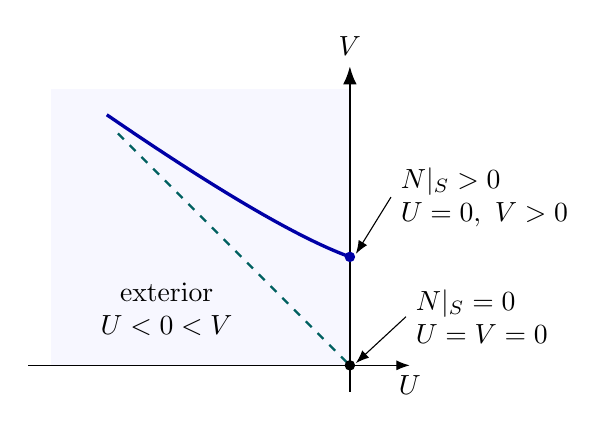
\begin{tikzpicture}[scale=0.95,>=Latex]
  \fill[blue!3] (-4,0) rectangle (0,3.7);
  \draw[->] (-4.3,0)--(0.8,0) node[below] {\(U\)};
  \draw[->,thick] (0,-0.35)--(0,4.0) node[above] {\(V\)};
  \draw[very thick,blue!65!black]
      (-3.25,3.35) .. controls (-1.5,2.15) and (-0.55,1.65)
                   .. (0,1.45);
  \draw[thick,dashed,teal!75!black] (-3.1,3.1)--(0,0);
  \fill[blue!65!black] (0,1.45) circle (2pt);
  \fill (0,0) circle (2pt);
  \node[align=left,anchor=west] (future) at (0.55,2.25)
      {\(N|_S>0\)\\\(U=0,\ V>0\)};
  \draw[->] (future.west)--(0.08,1.49);
  \node[align=left,anchor=west] (bif) at (0.75,0.65)
      {\(N|_S=0\)\\\(U=V=0\)};
  \draw[->] (bif.west)--(0.08,0.03);
  \node[align=center] at (-2.45,0.75)
      {exterior\\\(U<0<V\)};
 \end{tikzpicture}
 \caption{The two smooth horizon attachments in
 \eqref{k:null-coordinates}, with angular directions suppressed.
 The curves depict alternative spacelike slices. In the
 positive-lapse case the boundary value of \(V\) may vary over
 the horizon sphere, as in \eqref{k:future-graph}.}
 \label{k:horizon-figure}
\end{figure}

\subsection{The converse for arbitrary admissible slices}

For a \KN{} spacetime whose parameters have already been
identified with \(m,J,Q_e,Q_b\), every smooth cross-section of
the indicated horizon has area
\begin{equation}\label{k:horizon-area}
 A_H=4\pi\left[
 \left(m+\sqrt{m^2-(J/m)^2-Q^2}\right)^2+(J/m)^2\right].
\end{equation}
Indeed the horizon is nonexpanding and its null induced metric
descends to its sphere of generators. The area is independent
of the section. Substitution in the parameter identity of
Lemma~\ref{a:model-parameters} gives equality in Theorem~\ref{m:main}.
This applies to nonconstant time graphs as well.

We supply the end identification also when an embedding into a
subextremal \KN{} exterior is given without initially equating
its ambient parameters with the fluxes of the slice. This
ensures that the converse uses exactly the asymptotic frame in
the theorem.

\begin{lemma}\label{k:end-identification}
Let an original, unpolarized data set satisfying the asymptotic
and rest-frame hypotheses of Theorem~\ref{m:main} be realized
as a spacelike slice approaching spatial infinity in a
subextremal \KN{} exterior with parameters
\(M,\widetilde a,\widetilde Q_e,\widetilde Q_b\). Then
\[
 m=M,\qquad J^2=M^2\widetilde a^2,\qquad
 Q_e^2+Q_b^2=\widetilde Q_e^2+\widetilde Q_b^2 .
\]
In a sufficiently distant stationary spatial chart the slice
is a single graph \(t=F(\bar x)\), with
\(\dd F=O_1(|\bar x|^{-2})\).
\end{lemma}

\begin{proof}
Write \(r_x=|x|\) in the prescribed slice chart, let \(T\) be
the stationary time Killing field future at infinity, and
decompose
\[
 T=N_Tn+Y_T .
\]
Since the end approaches ambient spatial infinity,
\(N_T>|Y_T|_g\) eventually and
\(N_T^2-|Y_T|_g^2=-\bar g(T,T)\to1\).
We first obtain
\begin{equation}\label{k:restricted-killing}
 N_T\to1,\qquad Y_T=O_2(r_x^{-2}).
\end{equation}
No prior bound on the tilt of the embedding is needed.
The Gauss equation bounds the tangential ambient curvature
components in the slice frame by \(O(r_x^{-3})\); Codazzi
bounds the components with one normal index by the same order.
The remaining normal-normal block follows by contraction
with the ambient Ricci tensor, whose components in this
frame are \(O(r_x^{-4})\) by the given electromagnetic fields
and the Einstein--Maxwell equation. Thus
\(\overline{\operatorname{Rm}}=O(r_x^{-3})\) in the entire
slice frame.

The Killing first-jet equation
\(\bar\nabla^2T=\overline{\operatorname{Rm}}*T\), split into
tangential and normal components, therefore has the end
bounds used in Lemma~\ref{j:end}. The splitting adds only
\(K*\bar\nabla T\) and
\((\nabla K+K*K)*T\); the skew symmetry of \(\bar\nabla T\)
controls all its components by the tangential derivatives.
In slice coordinates the Christoffel symbols and their
derivatives are \(O(r_x^{-2})\), \(O(r_x^{-3})\).
The radial first-jet integration and causality argument of
that lemma consequently give constant limits with
\(O_2(r_x^{-q'})\) errors, for any fixed \(1/2<q'<1\).
Here the normalization is determined by
\(-\bar g(T,T)\to1\), rather than by a variational prototype.

For the original unpolarized data, the constraints and prescribed falloff give
\[
 L(g-\delta)=\partial_i\partial_j(g-\delta)_{ij}
       -\Delta_\delta\tr_\delta(g-\delta)=O(r_x^{-4}).
\]
The pair \((N_T,Y_T)\) satisfies
\(\operatorname{sym}\nabla Y_T=-N_TK\), with \(K=O_1(r_x^{-3})\),
bounded \(N_T\), and the constant asymptotics just proved. Since \(m>0\),
the general assertion of Lemma~\ref{j:end} gives \(Y_{T,\infty}=0\).
The norm limit then gives \(N_{T,\infty}=1\).
Prolonging \(\operatorname{sym}\nabla Y_T=-N_TK\) gives
\[
 |\partial^2Y_T|
 \le C r_x^{-2}|\partial Y_T|
       +Cr_x^{-3}|Y_T|+Cr_x^{-4}.
\]
Twice integrating from the zero end limits, and reinserting
the improved bounds, yields \eqref{k:restricted-killing}.

Project along \(T\) to stationary spatial coordinates
\(\bar x\) of the ambient exterior, and restrict to
\(\bar r=|\bar x|\) sufficiently large. This projection is a
local diffeomorphism on the slice, because a timelike vector
cannot be tangent to a spacelike hypersurface. It is proper
over that spatial tail: the end goes to ambient spatial
infinity, and a compact core has bounded projected radius.
Explicitly, for every ambient radius \(R\) there is a slice
radius \(R_x(R)\) such that
\[
 |x|>R_x(R)\quad\Longrightarrow\quad |\bar x|>R.
\]
Thus the preimage of the ambient tail contains one whole
connected intrinsic coordinate tail, and the preimage of
any compact subset of the ambient tail is a closed subset
of an intrinsic compact set.
Its image is therefore open and closed in the connected
tail, so it is surjective and a covering. The spatial tail
is simply connected. Each component of its preimage covers
the whole tail and hence reaches arbitrarily far out in
the slice end: otherwise its closure would lie in an
intrinsic compact set, whose projected radius is bounded.
All such components must therefore intersect the one
connected full intrinsic tail just specified. There is just
one component and one sheet. This proves the single-graph
assertion.

The stationary orbit metric on this three-dimensional end
pulls back to
\begin{equation}\label{k:orbit-metric}
 g_T=g+\frac{(Y_T^\flat)^2}{N_T^2-|Y_T|^2}.
\end{equation}
By \eqref{k:restricted-killing}, it differs from \(g\) by
\(O_2(r_x^{-4})\) and has the same mass.
In the ambient stationary chart, the same metric differs
from the canonical spatial metric by
\(\bar g_{ti}\bar g_{tj}/(-\bar g_{tt})=O_2(\bar r^{-4})\).
The canonical mass is \(M\).

Here the equality of masses in the two charts can be checked
directly. Since both represent the same uniformly Euclidean
metric, \(D\bar x\) and its inverse are bounded. Distances in
the two ends show that \(r_x\) and \(\bar r\) are comparable.
The transformation law for the Christoffel symbols then
gives \(D^2\bar x=O(r_x^{-2})\). Integrating along rays and
sphere paths yields a constant orthogonal matrix \(O_*\) with
\begin{equation}\label{k:chart-transition}
 D\bar x=O_*+O(r_x^{-1}),\qquad
 \bar x=O_*x+O(\log r_x).
\end{equation}
The ADM flux comparison separates a pure Euclidean
symmetric gradient, whose linear flux vanishes, from the
original perturbation. Quadratic errors tend to zero.
The Euclidean scalar linearization is integrable
(\(O(r_x^{-4})\)), so asymptotically round deformed spheres
give the same limit as round spheres. Thus \(m=M\).

In the \(\bar x\)-chart the graph satisfies
\begin{equation}\label{k:graph-gradient}
 \dd F=
 \frac{\bar g_{ti}\dd\bar x^i-Y_T^\flat}
                  {N_T^2-|Y_T|^2}
             =O_1(\bar r^{-2}).
\end{equation}
Its vanishing tilt leaves the leading Coulomb fluxes
unchanged, giving
\(Q_e^2+Q_b^2=\widetilde Q_e^2+\widetilde Q_b^2\);
possible orientation changes do not affect this identity.
The graph tangents and the normalized future normal
covector proportional to \(-\dd t+\dd F\) give, with the
positive convention for \(K\),
\begin{equation}\label{k:graph-tensor}
 K_{ij}=K^{\rm can}_{ij}+\partial_i\partial_jF
                                  +O(\bar r^{-4}).
\end{equation}
For every Euclidean rotation vector \(R\),
\[
 n_\delta^i(\partial_i\partial_jF)R^j
       =R\left(\partial_{\bar r}F-\frac{F}{\bar r}\right).
\]
Its round-sphere integral is zero because \(R\) preserves
the sphere area form. The trace-reversed Euclidean term
also vanishes, since \(R\) is tangential; all metric,
normal, and area errors tend to zero at these decay orders.
Hence the angular flux vector in this chart has the
canonical norm \(|M\widetilde a|\).

Under \eqref{k:chart-transition}, rotation vectors agree,
up to the constant orthogonal change, with errors
\(O(\log r_x)\). Their flux errors are
\(O(\log r_x/r_x)\), since \(K=O_1(r_x^{-3})\).
The corresponding spheres differ in radius by
\(O(\log r_x)\), and their normals and relative area
elements by \(O(\log r_x/r_x)\); these also give vanishing
angular-flux errors. In the prescribed slice chart,
axisymmetry forces the two transverse components of the
angular flux vector to vanish. Its axial component is
the prescribed total \(J\), because the electromagnetic
correction tends to zero at infinity. Thus its norm is
\(|J|\), proving \(J^2=M^2\widetilde a^2\).
\end{proof}

If an admissible embedded slice is only said to meet the
appropriate future horizon, its boundary is nevertheless a
cross-section. An interior point cannot lie on the null face,
by spacelikeness and the fact that the whole image lies on its
exterior side. At a boundary contact use the smooth horizon
coordinate \(U\), with \(U=0\) on the future branch,
\(U<0\) in the exterior, and \(\dd U\) positive on future
timelike vectors. Extend the spacelike embedding locally a
little beyond its boundary; spacelikeness is an open condition.
The cut \(U=0\) of this extension is a smooth MOTS with normal
toward \(U<0\): its outgoing future null direction is tangent
to the nonexpanding horizon. This remains true at bifurcation.
The given \(S\) touches this cut from the exterior side with
the same outward orientation. Local graph strong comparison
for the expansion equation makes the surfaces coincide near
the contact. The contact set is therefore open and closed
in the connected \(S\), so all of \(S\) lies on that branch.
Projection along the horizon generators is a local
diffeomorphism by spacelikeness. Compactness makes it a
covering of the generator sphere, and simple connectivity
makes it a diffeomorphism. Formula~\eqref{k:horizon-area},
with the parameter identifications of
Lemma~\ref{k:end-identification}, now proves the converse.

\begin{lemma}[Exclusion of partial bifurcation contact]
\label{k:horizon-cut-dichotomy}
A smooth spacelike cross-section of the closed future horizon bounding an exterior
with \(\theta_+=0\) and the all-cut outer area-minimizing property
lies entirely on the open future horizon or is the bifurcation
sphere.
\end{lemma}

\begin{proof}
This is a direct boundary argument, independent of the adjoint
boundary dichotomy. In the smooth co-rotating coordinates
\eqref{k:null-coordinates}, write the section as
\(U=0,\ V=v(x)\ge0\), where \(x\) ranges over the sphere of
generators. Such a global graph exists because generator
projection is a diffeomorphism.
Smoothness of the model coefficients in \(-UV\), with the
weights imposed by the horizon Killing field
\(\kappa(-U\partial_U+V\partial_V)\), gives on \(U=0\)
\[
 \bar g_{UV}=-c,\quad
 \bar g_{UA}=Vb_A,\quad
 \bar g_{AB}=q_{AB},\quad
 \bar g_{VA}=\bar g_{VV}=0,\qquad c>0,
\]
and
\[
 \partial_U\bar g_{AB}=Vd_{AB},\qquad
 \partial_U\bar g_{VA}=e_A,\qquad
 \partial_U\bar g_{VV}=0.
\]
Here \(q\) is a positive sphere metric and all coefficients
are smooth functions of \(x\). The last identity follows from
the stronger form \(\bar g_{VV}=U^2a_2(UV,x)\); merely knowing
\(\bar g_{VV}=0\) on the horizon would not suffice.

Set \(\ell=\partial_V\), and choose the transverse future null
normal \(k\) with \(\bar g(k,\ell)=-1\). The section tangents
are \(e_A^{\,S}=\partial_A+v_A\partial_V\); orthogonality gives
\[
 k^U=\frac1c,\qquad
 k^A=q^{AB}\left(v_B-\frac{v b_B}{c}\right),\qquad
 k_V=-1,\qquad k_A=v_A.
\]
The remaining component is fixed by nullness and is immaterial
for the expansion because the horizon's outgoing second
fundamental form is zero. Direct contraction of
\(-\bar g(k,\bar\nabla_{e_A^{\,S}}e_B^{\,S})\) with \(q^{AB}\)
gives the linear expression
\begin{equation}\label{k:cut-expansion}
 \theta_k[v]=
 \Delta_q v+
 \frac1c\langle\dd c+e-b,\dd v\rangle_q+
 \frac{\tr_qd-2\operatorname{div}_q b}{2c}\,v .
\end{equation}
For example the relevant lower Christoffel coefficients are
\[
 \Gamma_{U;AB}
    =\frac V2(\partial_A b_B+\partial_B b_A-d_{AB}),\qquad
 \Gamma_{U;VB}
    =\frac12(b_B-\partial_Bc-e_B);
\]
combining these with \(k_V=-1\), \(k_A=v_A\) yields
\eqref{k:cut-expansion}. The \(VV\) coefficients vanish on
the horizon, so there is no quadratic gradient term.

Outer area minimization, applied to arbitrary nonnegative
outward variations, implies \(H\ge0\). Since
\(\theta_+=H+\tr_SK=0\), the other future expansion is
\(\theta_-=\tr_SK-H=-2H\le0\).
The outward future normal \(n+\nu\) is a positive multiple
of \(\ell\), so \(n-\nu\) is a positive multiple of \(k\).
Consequently \(\theta_k[v]\le0\).
Equation~\eqref{k:cut-expansion} is a uniformly elliptic
linear inequality for the nonnegative smooth function \(v\).
The strong minimum principle applies even if its zeroth-order
coefficient has either sign: in the operator
\(-\theta_k\), replace that coefficient by its positive part,
which preserves the supersolution inequality because
\(v\ge0\). Hence a zero of \(v\) forces \(v\equiv0\) on the
connected sphere. Otherwise \(v>0\) everywhere, proving the
two alternatives.
\end{proof}

\subsection{Sharp examples and completion of the proof}

The canonical constant Boyer--Lindquist-time slice
\(\sigma\ge0\) provides a sharp example for every subextremal
choice of parameters on the strict branch. Its topology is
the rotation exterior, and it is complete with its compact
boundary included. In the Euclidean end radius
\(\rho_0=(b/2)e^\sigma\), the model metric has Cartesian
expansion
\[
 g^{\rm can}_{ij}
   =\left(1+\frac{2M}{\rho_0}\right)\delta_{ij}
                                        +O_4(\rho_0^{-2}).
\]
The angular shift is \(O(\rho_0^{-3})\), so
\(K^{\rm can}=O_3(\rho_0^{-3})\). The electric model potential
has time coefficient \(Q/r+O(r^{-3})\) and spatial angular
coefficient \(O(r^{-1})\sin^2\vartheta\). It gives the required
radial Coulomb electric term and \(O_3(\rho_0^{-3})\) magnetic
field; inverse duality gives both prescribed charges.
All differentiated bounds follow by smooth expansion in
\(\rho_0^{-1}\) with ordinary polar parity. The bifurcate
coordinates used above prove inner-boundary regularity.
The source-free constraints, integrability, and
\(P_{\rm ADM}=0\) follow, with energy \(M\), angular momentum
\(-aM\), and the specified charges.

We verify the two geometric boundary hypotheses for these
examples, including cuts that are neither invariant nor
trapped. On the \(\sigma\)-spheres, the tangential trace of
\(K^{\rm can}\) is zero, because its only nonzero entries
are mixed azimuthal entries. For the smooth outward unit
radial field \(V_r=P^{-1/2}\partial_\sigma\),
\begin{equation}\label{k:radial-expansion}
 \theta_+=H=\divg V_r
       =\frac{\partial_\sigma W}{2W\sqrt P}.
\end{equation}
This is zero at \(\sigma=0\) and positive outside. Indeed,
\[
 \partial_rW
 =4r(r^2+a^2)-2a^2(r-M)\sin^2\vartheta
 \ge4r^3+2a^2(r+M)>0 ,
\]
and \(\partial_\sigma r=b\sinh\sigma>0\) outside.
At a largest-radius point of an enclosing interior surface,
the outward tangent normal is \(V_r\) and its mean curvature
is at least that of the tangent radial leaf. The tangential
planes, hence their \(K\)-traces, agree at that point.
Equation~\eqref{k:radial-expansion} therefore excludes every
compact enclosing surface with \(\theta_+\le0\) everywhere,
also when it has several components.

Finally let \(D\) be any enclosing end-side domain in the
definition of Theorem~\ref{m:main}, with full intrinsic
boundary \(\Gamma\), and let \(n_D\) point out of \(D\).
Truncate the whole exterior and \(D\) at a common distant
radial sphere. Subtracting their divergence identities gives
\[
 0\le\int_{\Omega\setminus D}\divg V_r\,\dd V_g
      =-A(S)-\int_\Gamma\langle V_r,n_D\rangle\,\dd A_g.
\]
The identity counts portions of \(\Gamma\) coinciding with
\(S\), including the case \(D=\Omega\). Since \(|V_r|=1\),
\[
 A(S)\le-\int_\Gamma\langle V_r,n_D\rangle\,\dd A_g
                                         \le\Area_g(\Gamma).
\]
Thus the canonical horizon is outer area-minimizing for the
full class of cuts.

\begin{proof}[Completion of Theorem~\ref{m:main}]
Corollary~\ref{d:numerical} proves the numerical inequality on
the closed physical branch. On the strict branch,
Proposition~\ref{j:adjoint} supplies the stationary quotient
and its boundary conditions. Lemmas~\ref{k:timelike}--\ref{k:rod-scale}
and Proposition~\ref{k:identification} identify that quotient
with the subextremal model determined by
Lemma~\ref{a:model-parameters}. Propositions~\ref{k:lift}
and~\ref{k:horizon} give the required smooth embedding of
the original metric, tensor, and electromagnetic fields,
with its future normal and its stated boundary image.
The horizon area formula and
Lemma~\ref{k:end-identification} prove the converse, and the
canonical examples verify sharpness within the stated class.
No classification on the extremal equality branch is asserted.
\end{proof}


\bibliographystyle{plain}
\bibliography{references}
\end{document}
